%!TEX root = ../thesis.tex
\chapter{Diffusion Smoothing Registration of High Resolution Rat Histology}
% If you like chapter abstracts ...
\dblspace
\begin{quote}{\em %!TEX root = ../thesis.tex

explicitly state what is my contribution. 
}\end{quote}

\section{Aims} % (fold)
\label{sec:aims}
  introductory motivational paragraph about problems with final affine result.

  Figure of zoomed in noise in HiRes result, and of intrinsic LoRes fixed image (jaggedness and changing light.)
  \subsection{Problem}
    \begin{itemize}
      \item Underlying noise in reference images, from changes in camera position and illumination angles and intensities
      \item Resolution of reference images are 8 times coarser at 8.8$\mu$ 
      \item Large discontinuities in camera position have already been corrected for in the block reference images, introducing the `banana problem' across the discontinuity
      \item Small non-rigid deformations when tissue is sliced and rehydrated, different in every slice and not fully represented by an affine transform.
      \item Registration close, but does not always find the global minimum.
    \end{itemize}

% section aims (end)

\section{Methods} % (fold)
\label{sec:methods}
  \subsection{A 1D Random Walk Analogy}
  The central limit theorem states that the mean of a sufficiently large number of independent random variables will be approximately normally distributed, regardless of their individual distribution. Indeed, Einstein's theory of the Brownian motion of a diffusive particle is based on this precept. With this in mind, the simplest model of microscopic diffusion is one in which a particle may move in a random walk in one dimension along the integer number line $\mathbb{Z}$, in steps of either $+1$ or $-1$, with equal probability. Taking each step as an independent random variable $Z_1, Z_2,\ldots$, if the particle's position $S$ starts at $S_0 = 0$, we can express the position of the particle after $N$ steps as
  \begin{equation}
    S_N = \sum\limits_{i=1}^N Z_i .
  \end{equation}
  The probability of taking $k$ positive steps out of a total of $N$ steps is given by
  \begin{equation}
    P(k;N) = \binom{N}{k}\left(\frac{1}{2} \right)^N,
  \end{equation}
  where the binomial coefficient
  \begin{equation}
    \label{eq:registration:binomial-coefficient}
     \binom{N}{k} = \frac{N!}{k!(N-k)!},
  \end{equation}
  since there are $\binom{N}{k}$ possible ways of taking $k$ and $N - k$ steps of $-1$ and $+1$, respectively. At each independent step, the probability of taking one or the other direction is $\frac{1}{2}$, leading to the product $\frac{1}{2}^N$.
  
  Applying Stirling's approximation:
  \begin{align}
    \label{eq:registration:stirling}
    \ln \left( n! \right) &= n\ln n - n + O(\ln n) \notag \\
           &\approx n\ln n - n \quad \text{as}\: n \to \infty,
  \end{align}
  
  \emph{Possibly include proof of de Moivre-Laplace theorem.}
  % Proof can be found here:
  % http://en.wikipedia.org/wiki/De_Moivre%E2%80%93Laplace_theorem
  We can see that in the limit of large $N$, the distribution of $k$ and thus $S_N$ tend to Gaussian:
  \begin{equation}
    \label{eq:registration:gaussian-approximation}
    \binom{N}{k}\left(\frac{1}{2}\right)^N \approx \sqrt{\frac{2}{\pi N}} \
      e^{-2(k - \frac{N}{2})^2/N}
  \end{equation}
  
  Show diagrams of half particles stepping once left, half right.
  
  It is clear from Equation~\ref{eq:registration:gaussian-approximation} that multiple application of this smoothing operation approximates a Gaussian diffusion smoothing.

  
  We might consider a concentration of particles $f$ over a discrete 1-dimensional grid $x$. After a discretised timestep $\Delta t$, a proportion $\alpha$ of the particles have taken a random walk, such that half of them have diffused to the left and half to the right:
  
  \begin{align}
    f(x_i, t_{n+1}) &= f(x_i, t_n) + \alpha (f(x_{i-1}, t_n) - 2f(x_i, t_n) + f(x_{i+1}, t_n)), \\
    \Delta f(x, t + \Delta t) &= \alpha (f(x - \Delta x, t) - 2f(x, t) + f(x + \Delta x, t)). \end{align}
  
  Figure of 1-D diffusion with alpha=0.4:
  \begin{figure}[htbp]
    \centering
		\subfigure[][]{\includegraphics[width=0.4\pagewidth]{Ch7/Figs/1d_noise/alpha_0.40/000}}
		\subfigure[][]{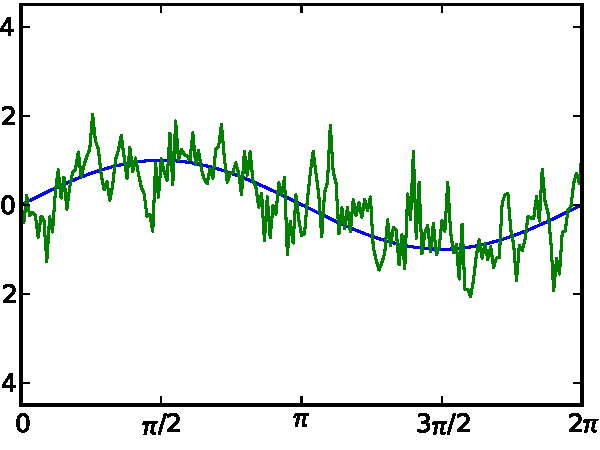
\includegraphics[width=0.4\pagewidth]{Ch7/Figs/1d_noise/alpha_0.40/001}}
		\subfigure[][]{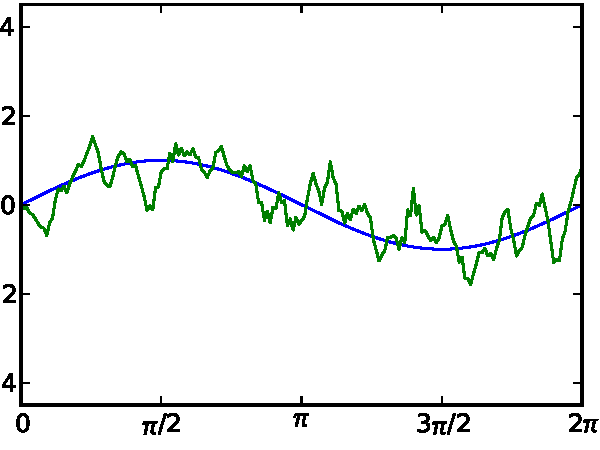
\includegraphics[width=0.4\pagewidth]{Ch7/Figs/1d_noise/alpha_0.40/003}}
		\subfigure[][]{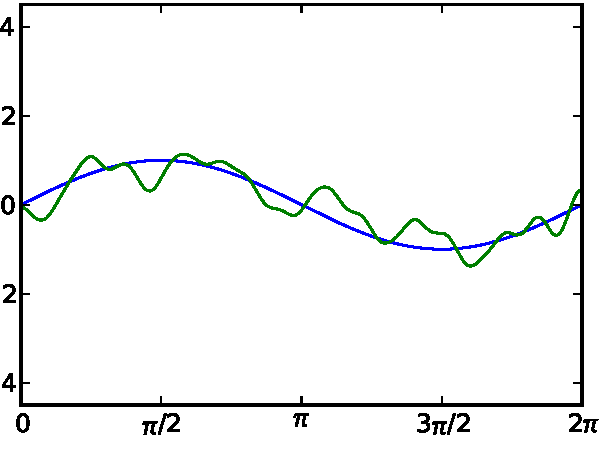
\includegraphics[width=0.4\pagewidth]{Ch7/Figs/1d_noise/alpha_0.40/015}}
		\subfigure[][]{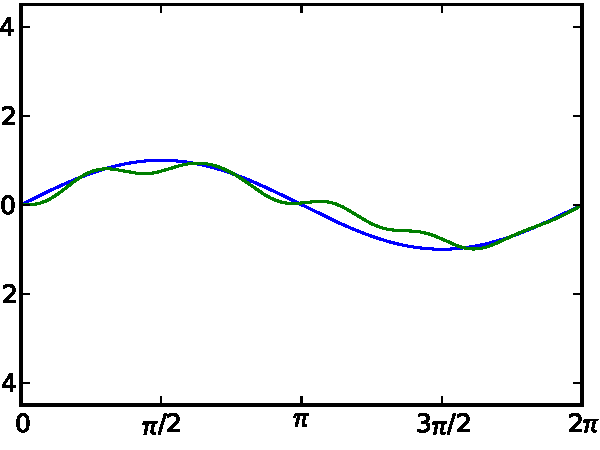
\includegraphics[width=0.4\pagewidth]{Ch7/Figs/1d_noise/alpha_0.40/099}}
		\subfigure[][]{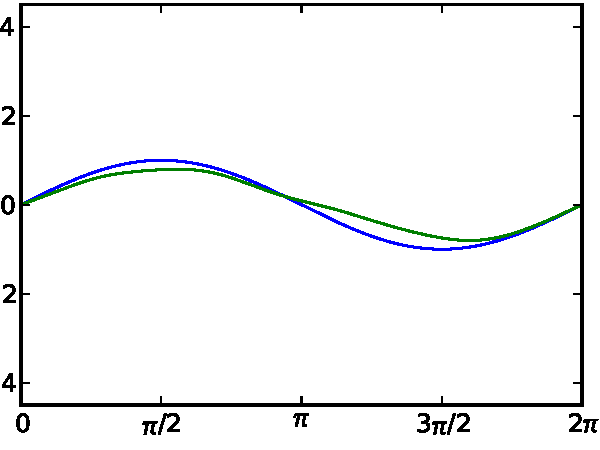
\includegraphics[width=0.4\pagewidth]{Ch7/Figs/1d_noise/alpha_0.40/299}}
    \caption{$\alpha = 0.4$. \textbf{(a)} Blah \textbf{(b)} blah blah Eq. \ref{eqn:potential}.}
	  \label{fig:1d_diffusion_0_40}
  \end{figure}

  Figure of 1-D diffusion with alpha=0.49:
  \begin{figure}[htbp]
    \centering
		\subfigure[][]{\includegraphics[width=0.4\pagewidth]{Ch7/Figs/1d_noise/alpha_0.49/000}}
		\subfigure[][]{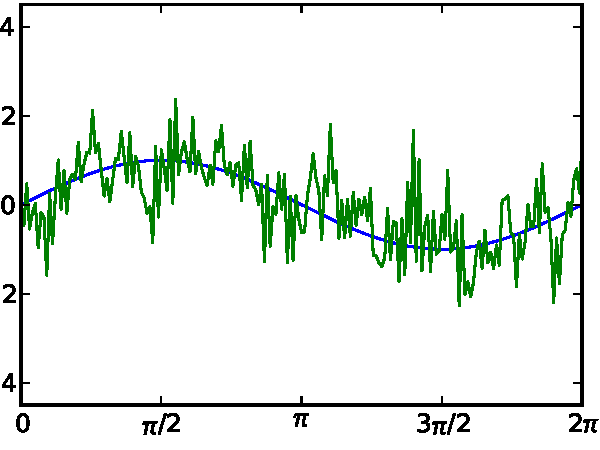
\includegraphics[width=0.4\pagewidth]{Ch7/Figs/1d_noise/alpha_0.49/001}}
		\subfigure[][]{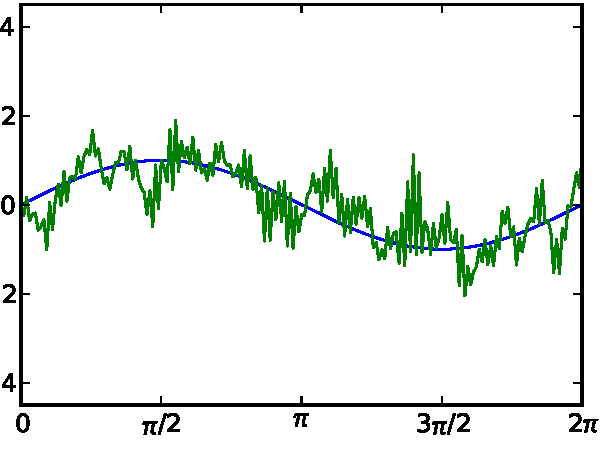
\includegraphics[width=0.4\pagewidth]{Ch7/Figs/1d_noise/alpha_0.49/003}}
		\subfigure[][]{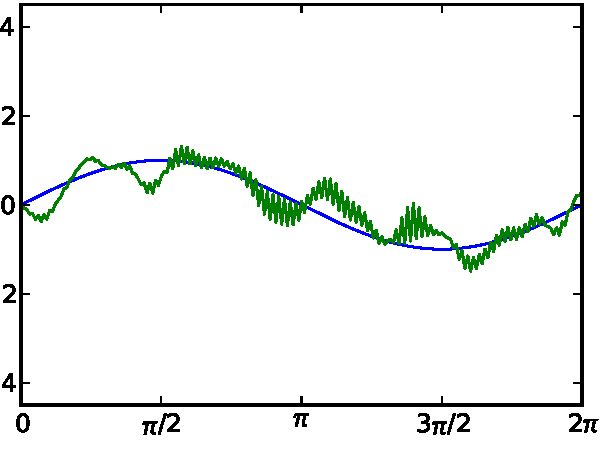
\includegraphics[width=0.4\pagewidth]{Ch7/Figs/1d_noise/alpha_0.49/015}}
		\subfigure[][]{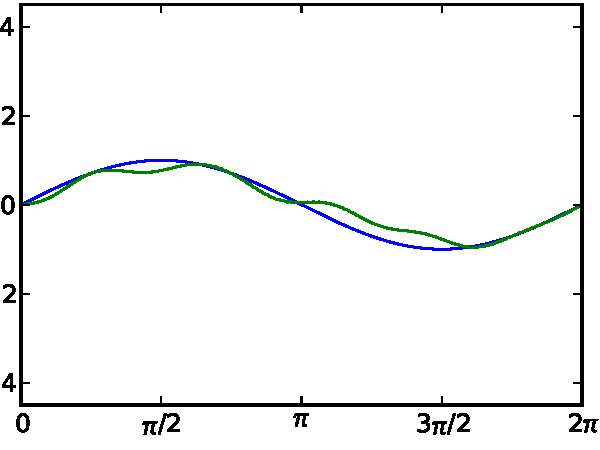
\includegraphics[width=0.4\pagewidth]{Ch7/Figs/1d_noise/alpha_0.49/099}}
		\subfigure[][]{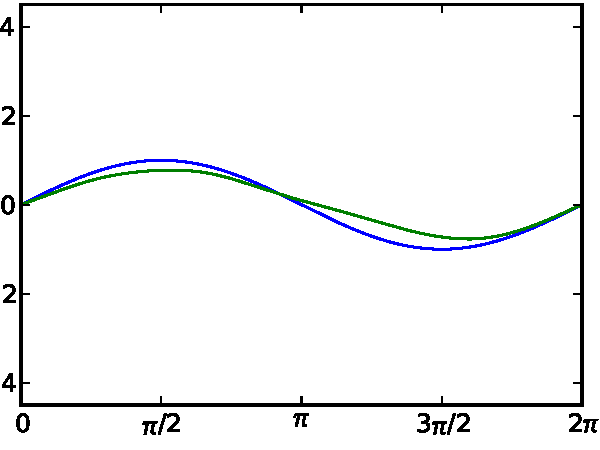
\includegraphics[width=0.4\pagewidth]{Ch7/Figs/1d_noise/alpha_0.49/299}}
    \caption{$\alpha = 0.49$. \textbf{(a)} Blah \textbf{(b)} blah blah Eq. \ref{eqn:potential}.}
	  \label{fig:1d_diffusion_0_49}
  \end{figure}
  
  Figure of 1-D diffusion with alpha=0.5:
  \begin{figure}[htbp]
    \centering
		\subfigure[][]{\includegraphics[width=0.4\pagewidth]{Ch7/Figs/1d_noise/alpha_0.50/000}}
		\subfigure[][]{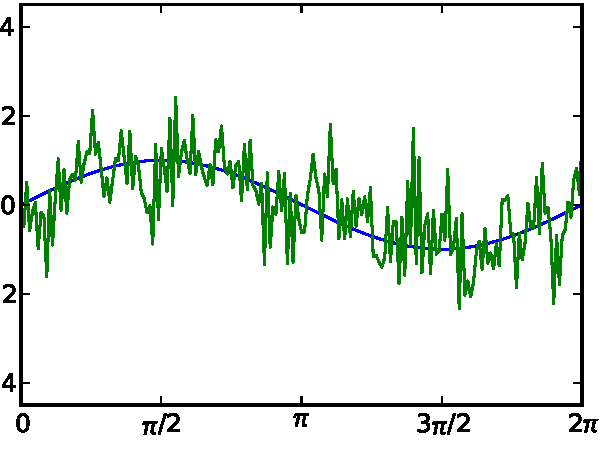
\includegraphics[width=0.4\pagewidth]{Ch7/Figs/1d_noise/alpha_0.50/001}}
		\subfigure[][]{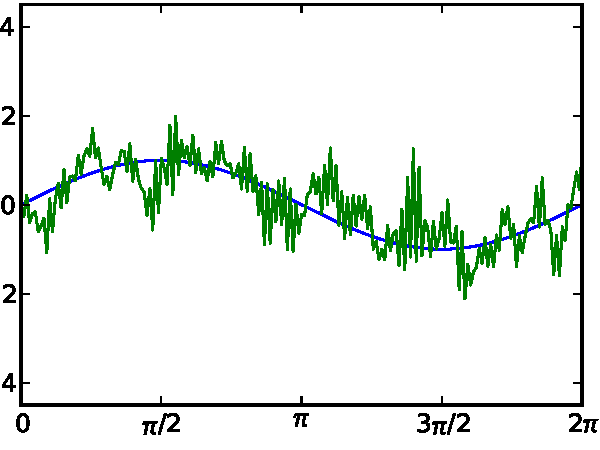
\includegraphics[width=0.4\pagewidth]{Ch7/Figs/1d_noise/alpha_0.50/003}}
		\subfigure[][]{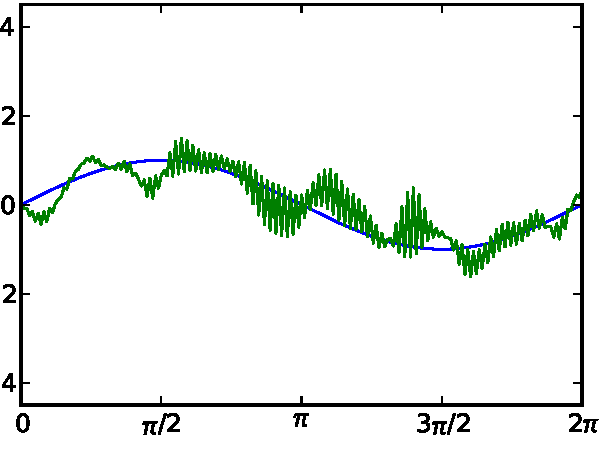
\includegraphics[width=0.4\pagewidth]{Ch7/Figs/1d_noise/alpha_0.50/015}}
		\subfigure[][]{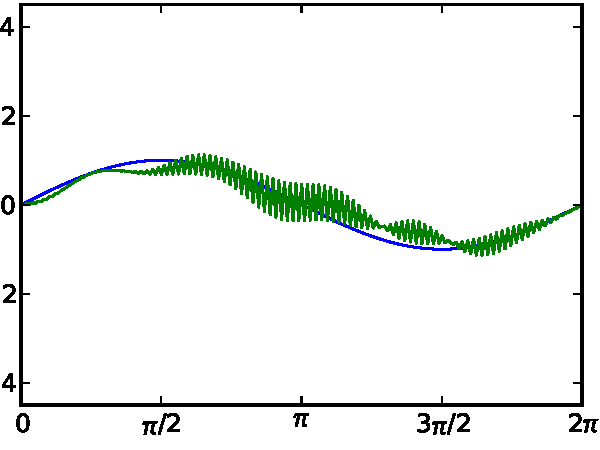
\includegraphics[width=0.4\pagewidth]{Ch7/Figs/1d_noise/alpha_0.50/099}}
		\subfigure[][]{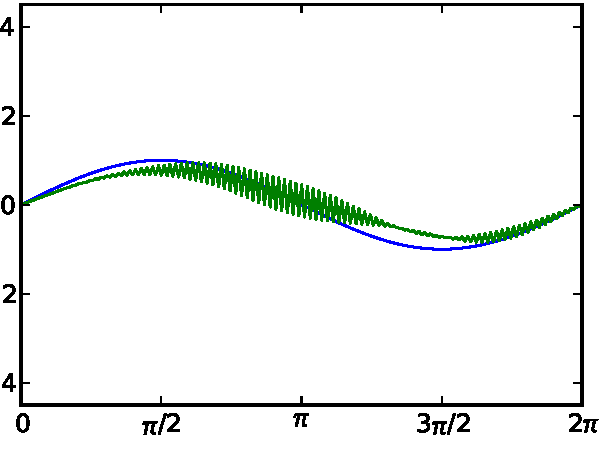
\includegraphics[width=0.4\pagewidth]{Ch7/Figs/1d_noise/alpha_0.50/299}}
    \caption{$\alpha = 0.5$. Equivalent to saying that all the particles move out of each bin.}
	  \label{fig:1d_diffusion_0_50}
  \end{figure}
  
  Figure of 1-D diffusion with alpha=0.51:
  \begin{figure}[htbp]
    \centering
  	\subfigure[][]{\includegraphics[width=0.4\pagewidth]{Ch7/Figs/1d_noise/alpha_0.51/000}}
  	\subfigure[][]{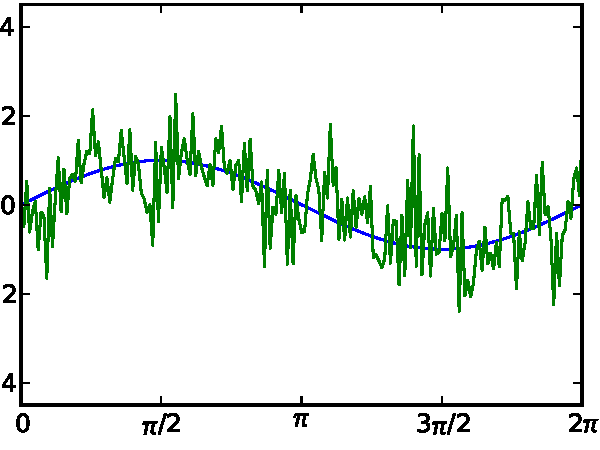
\includegraphics[width=0.4\pagewidth]{Ch7/Figs/1d_noise/alpha_0.51/001}}
  	\subfigure[][]{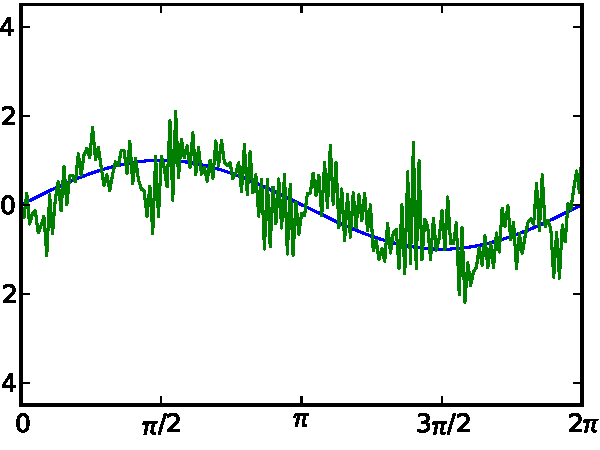
\includegraphics[width=0.4\pagewidth]{Ch7/Figs/1d_noise/alpha_0.51/003}}
  	\subfigure[][]{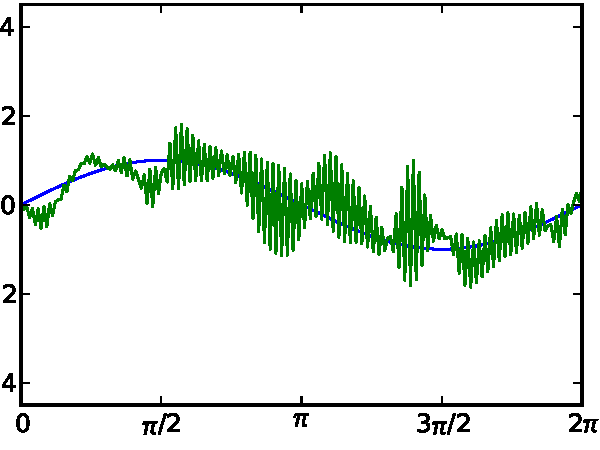
\includegraphics[width=0.4\pagewidth]{Ch7/Figs/1d_noise/alpha_0.51/015}}
  	\subfigure[][]{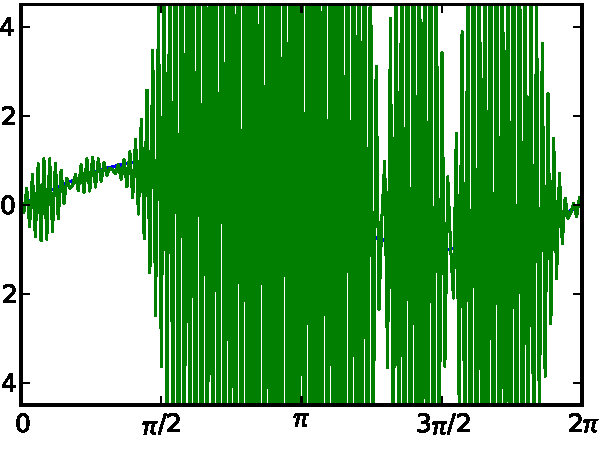
\includegraphics[width=0.4\pagewidth]{Ch7/Figs/1d_noise/alpha_0.51/099}}
  	\subfigure[][]{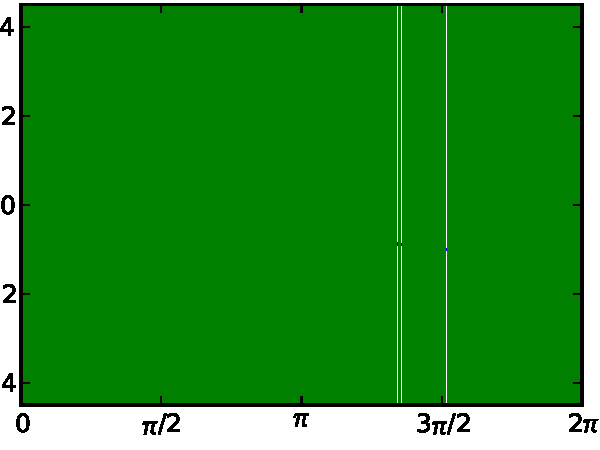
\includegraphics[width=0.4\pagewidth]{Ch7/Figs/1d_noise/alpha_0.51/299}}
    \caption{$\alpha = 0.51$. Unphysical, saying that more than all the particles move out of each bin.}
    \label{fig:1d_diffusion_0_51}
  \end{figure}
  
  
  Figure of Transformational diffusion from identity (use Seg3D slices and Paraview surfaces):
  % straight
  \begin{sidewaysfigure}[htbp]
    \centering
    % filename format: cross_section_200_alpha0.4_ITERATION_DIMENSION_SLICE
    \subfigure[][with noise (0 iterations)]{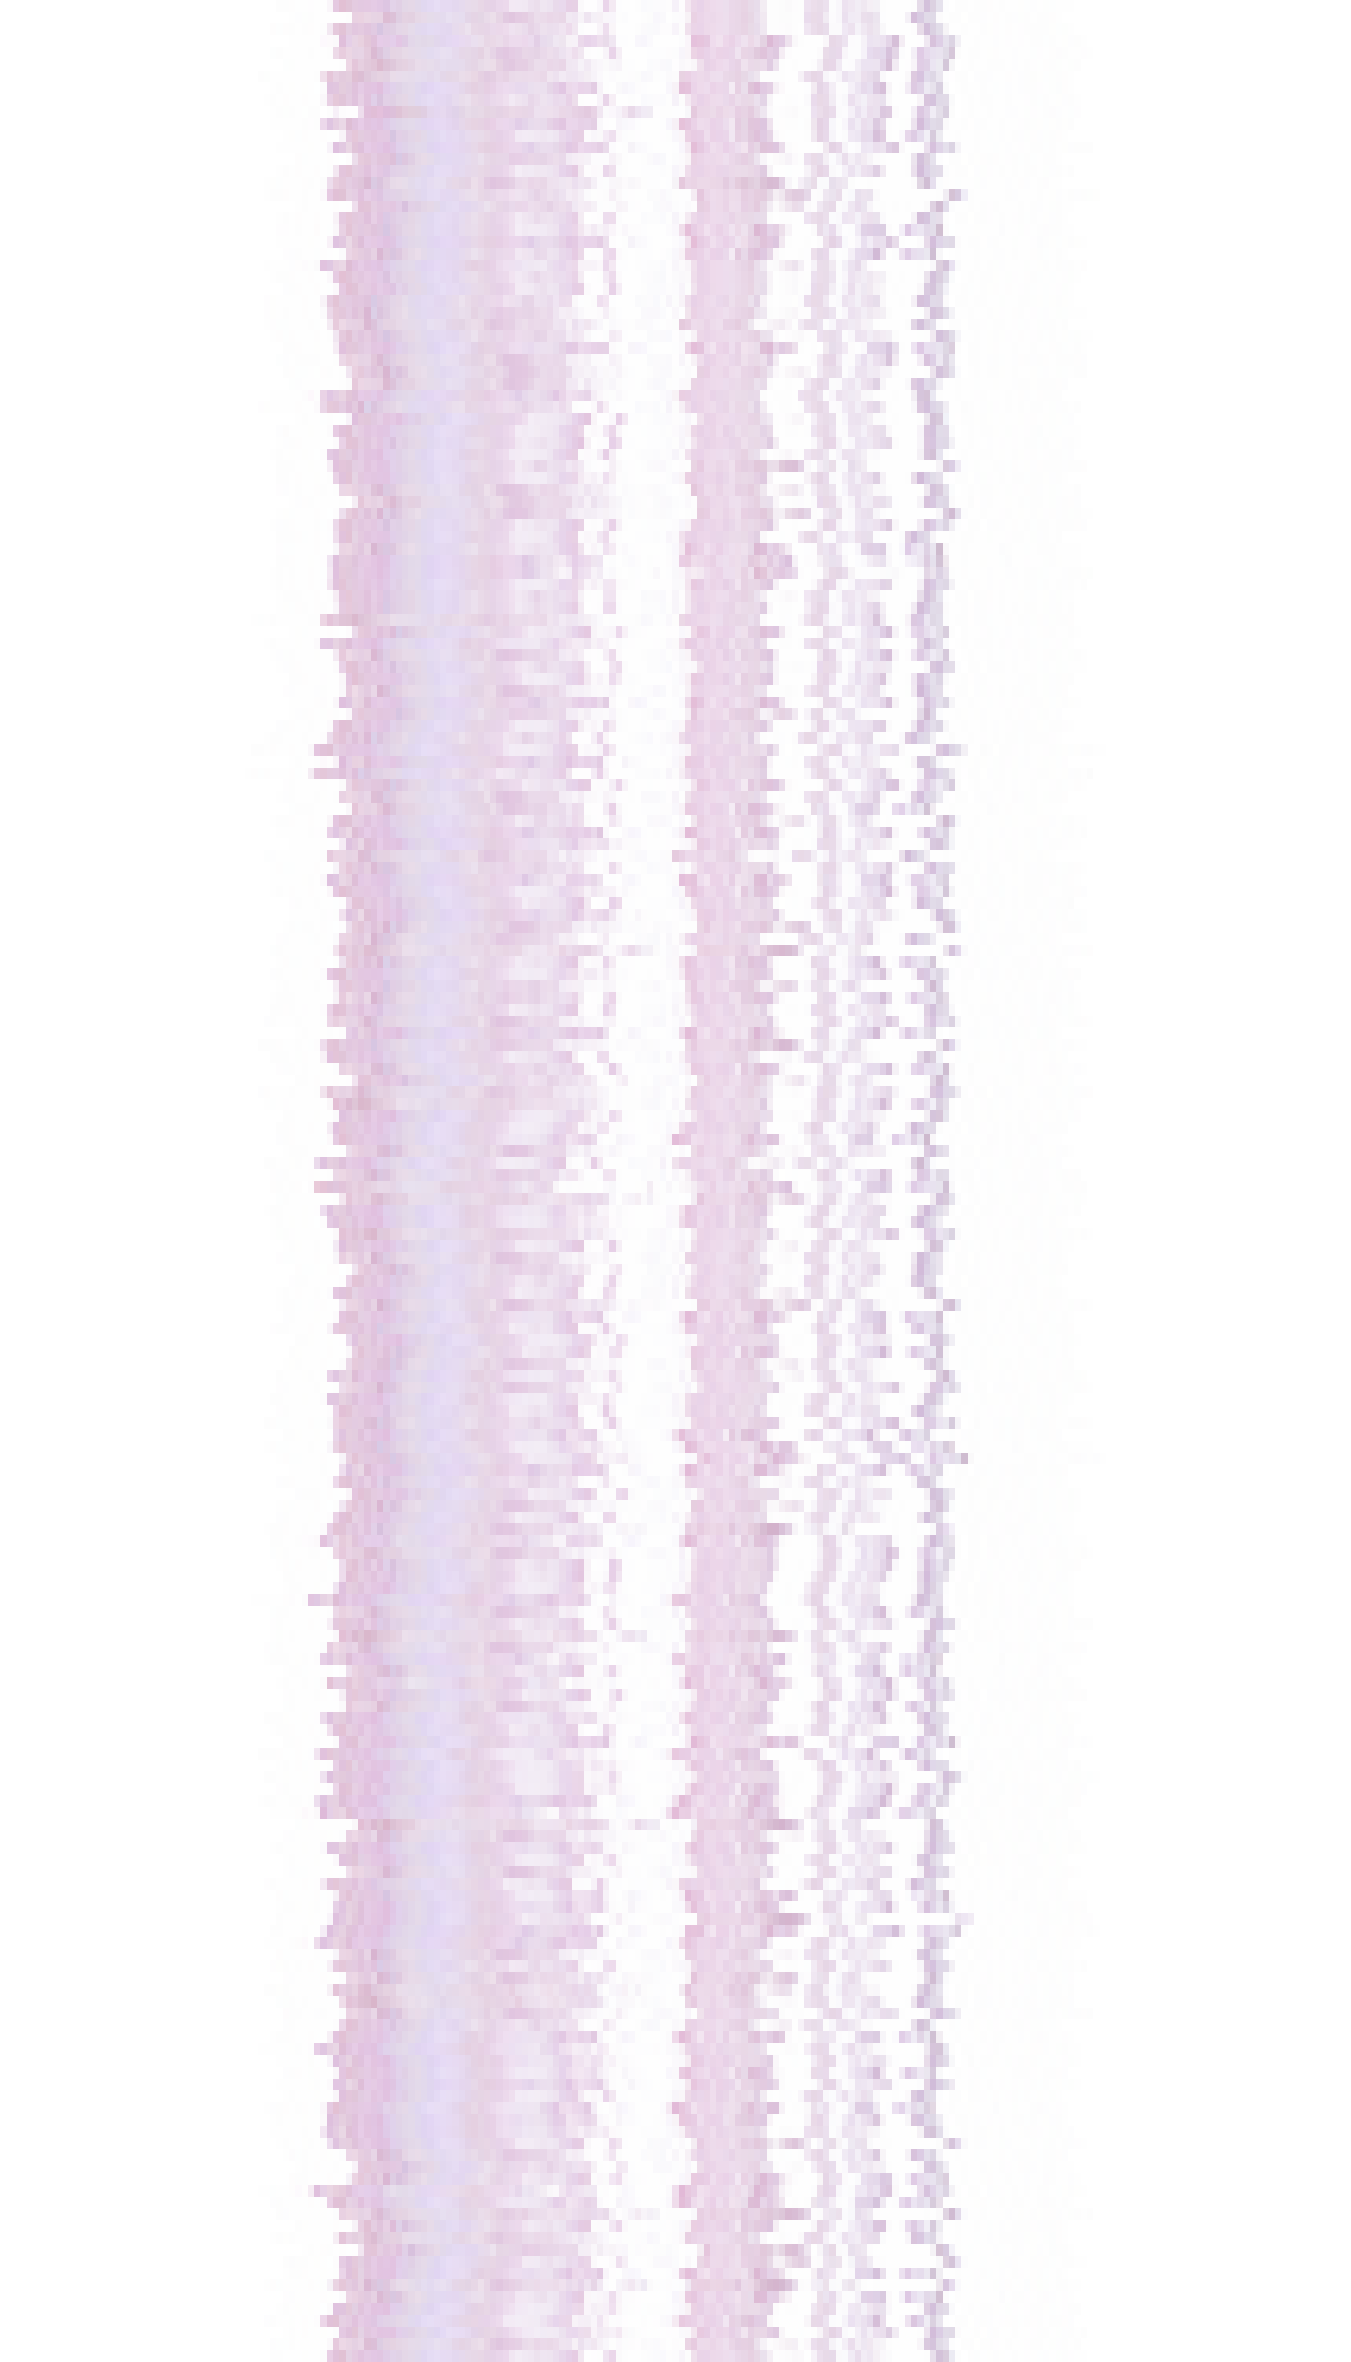
\includegraphics[height=0.33\textheight,type=pdf,ext=.pdf,read=.pdf]{Ch7/Figs/dummies/cross_section_200_alpha0.4_0_0_088}\label{fig:subfig1}}
    \subfigure[][1 iteration]{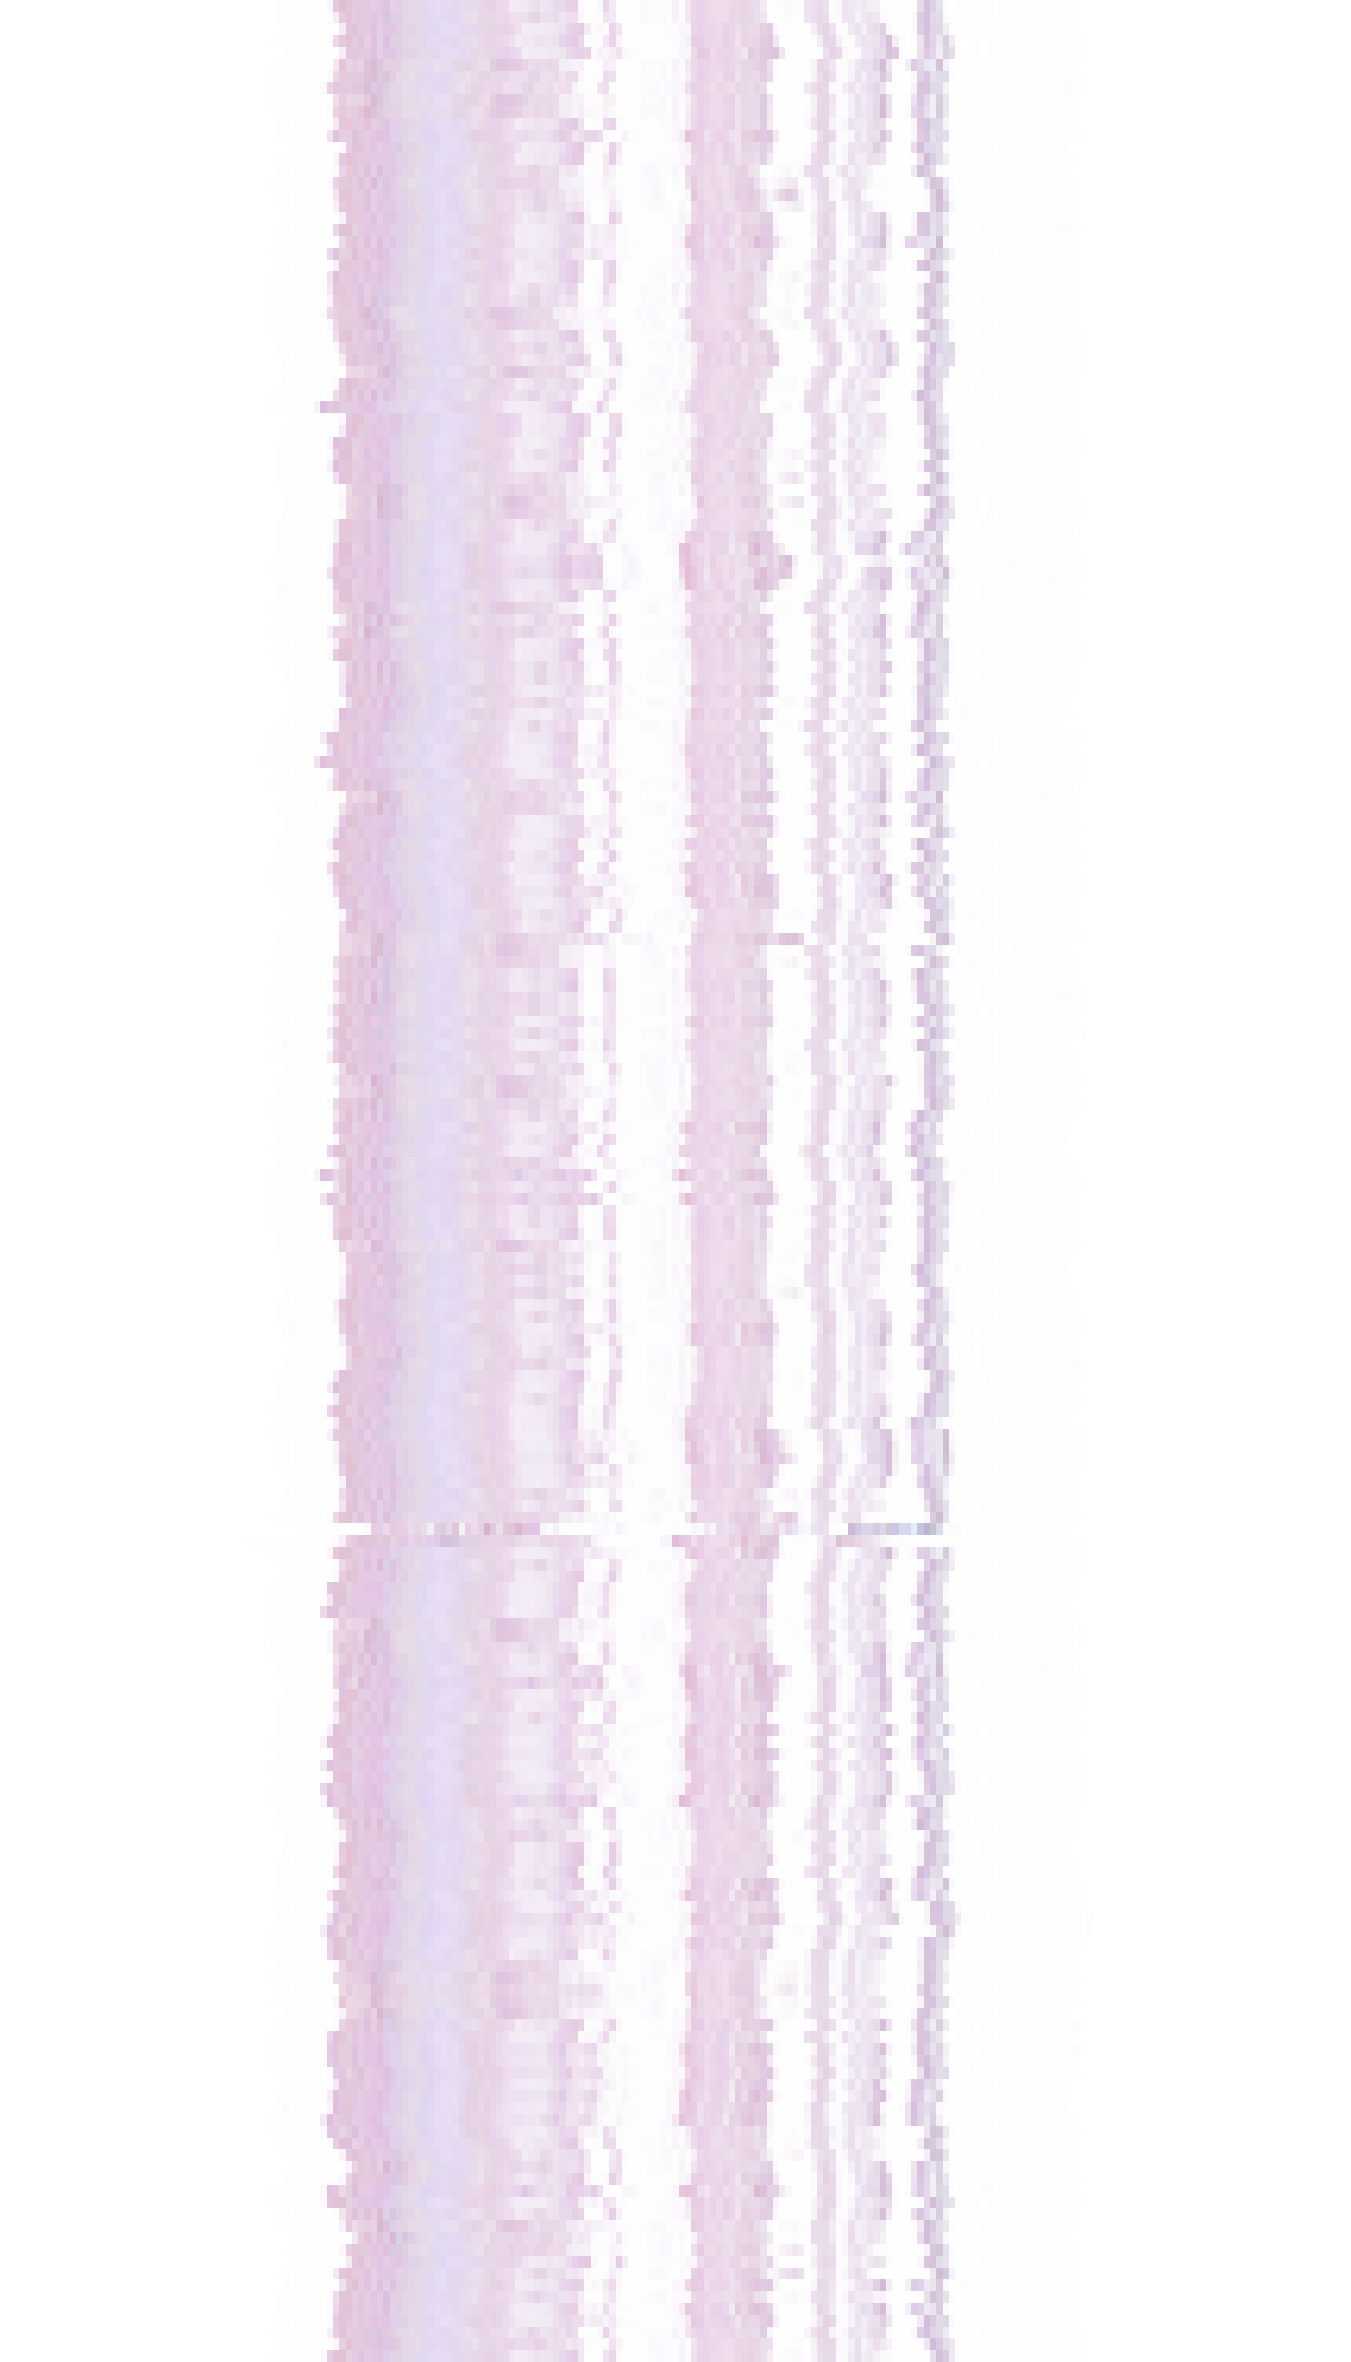
\includegraphics[height=0.33\textheight,type=pdf,ext=.pdf,read=.pdf]{Ch7/Figs/dummies/cross_section_200_alpha0.4_1_0_088}\label{fig:subfig2}}
    \subfigure[][3 iterations]{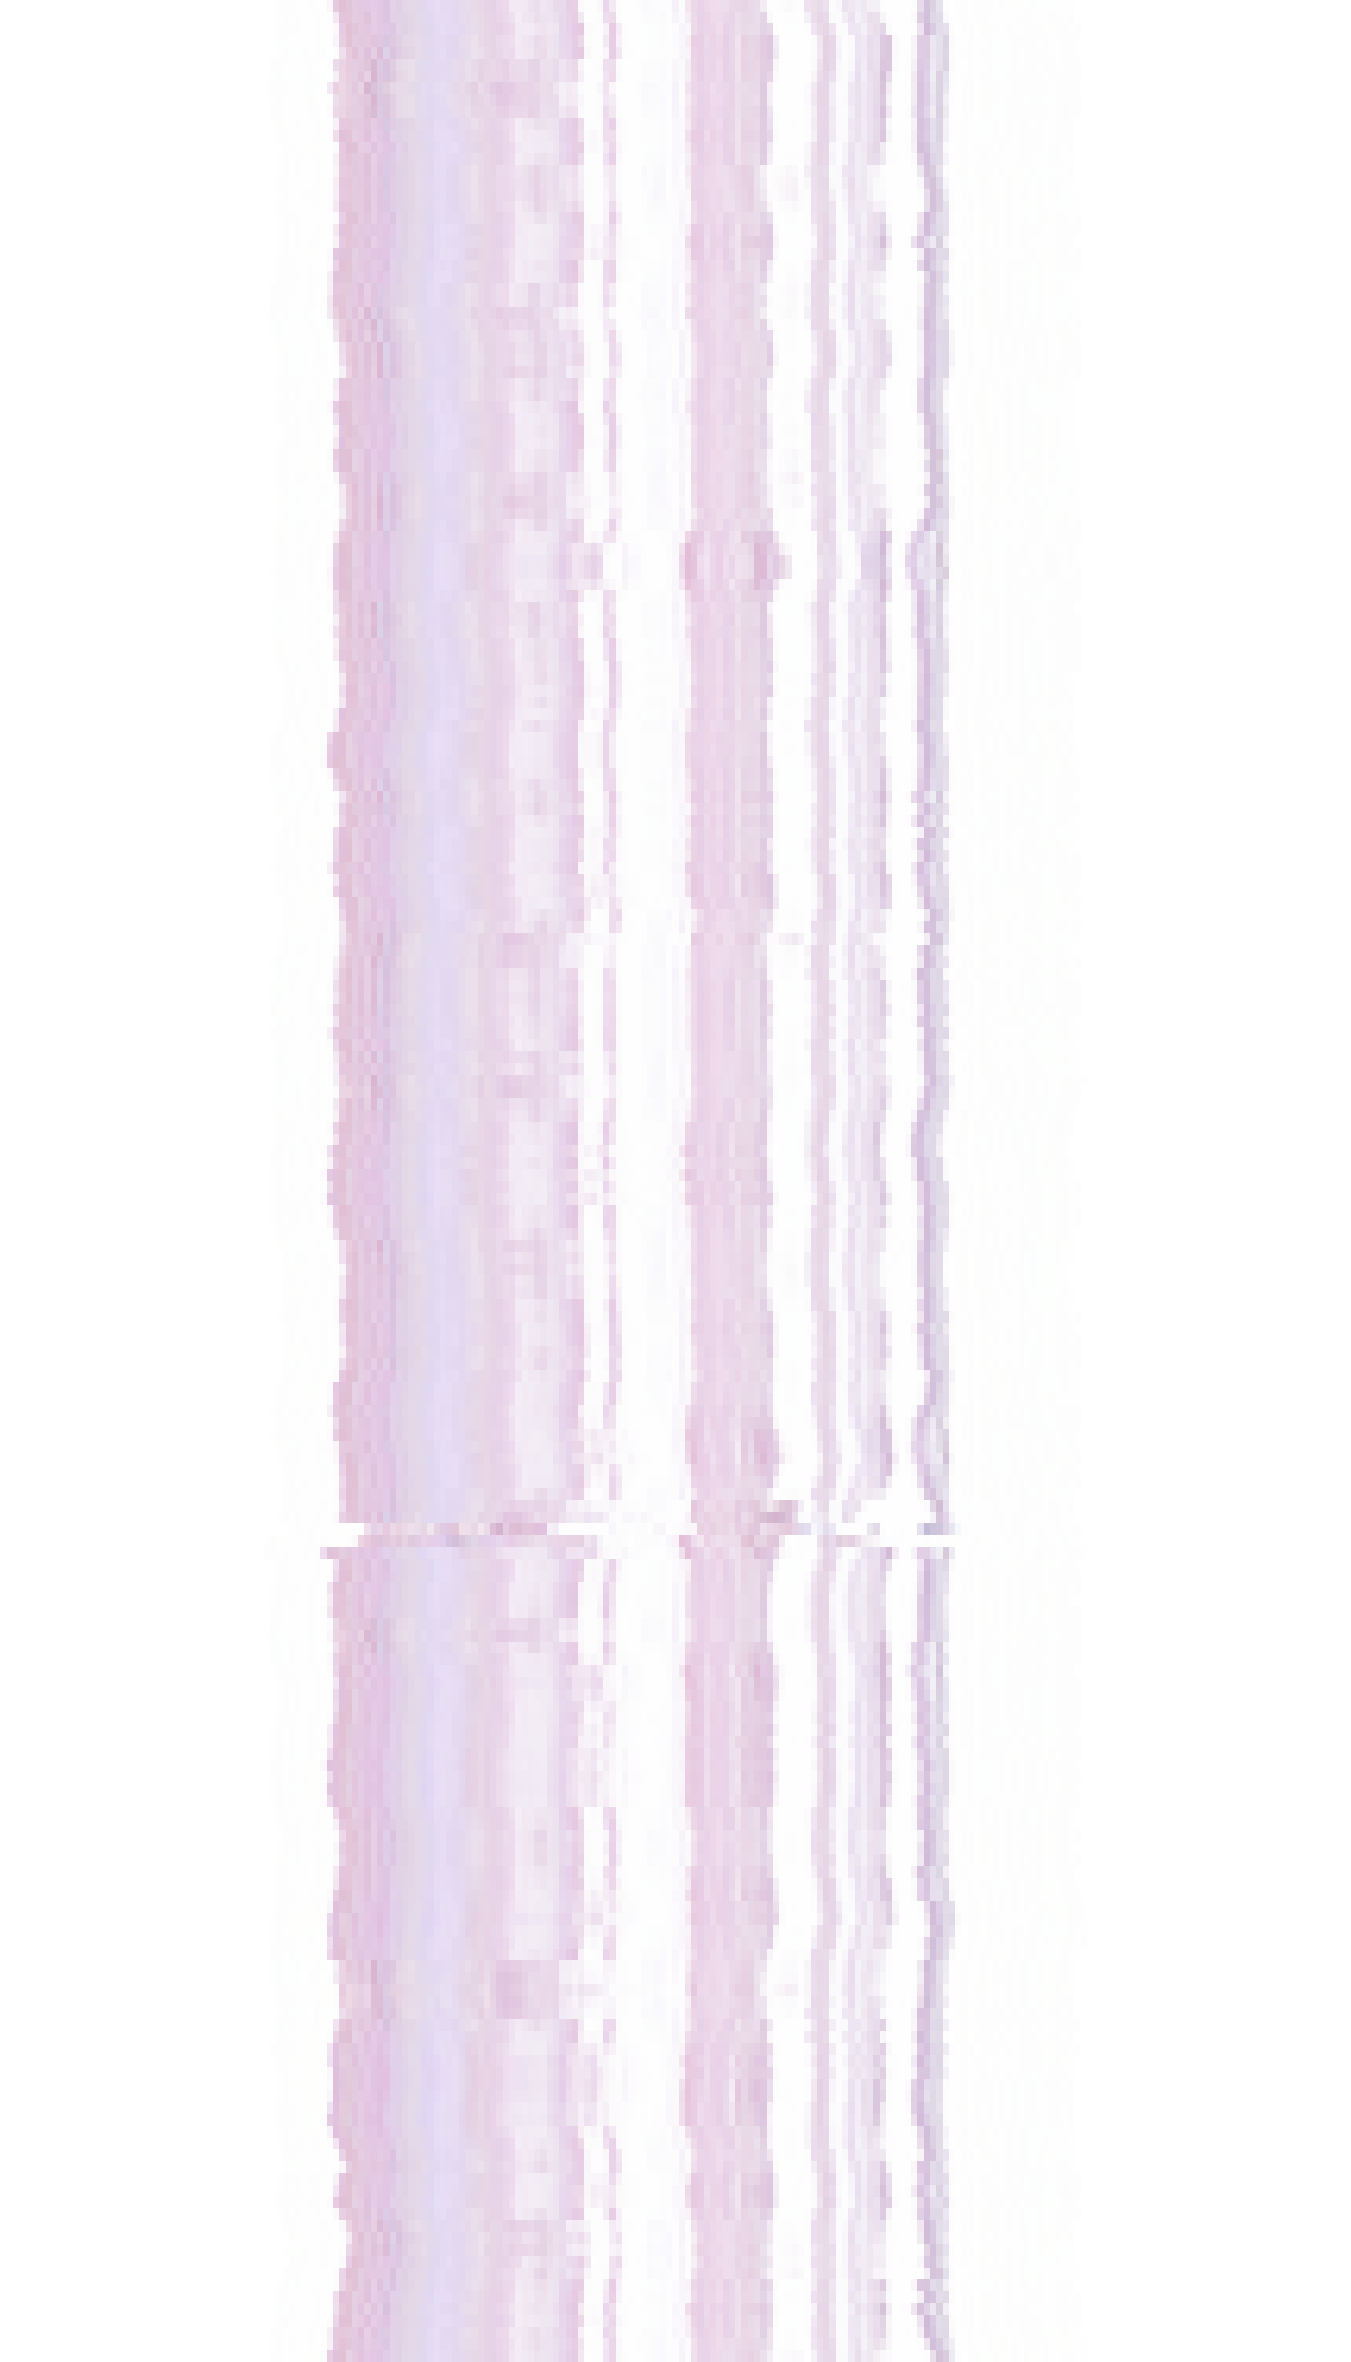
\includegraphics[height=0.33\textheight,type=pdf,ext=.pdf,read=.pdf]{Ch7/Figs/dummies/cross_section_200_alpha0.4_3_0_088}\label{fig:subfig3}}
    \subfigure[][10 iterations]{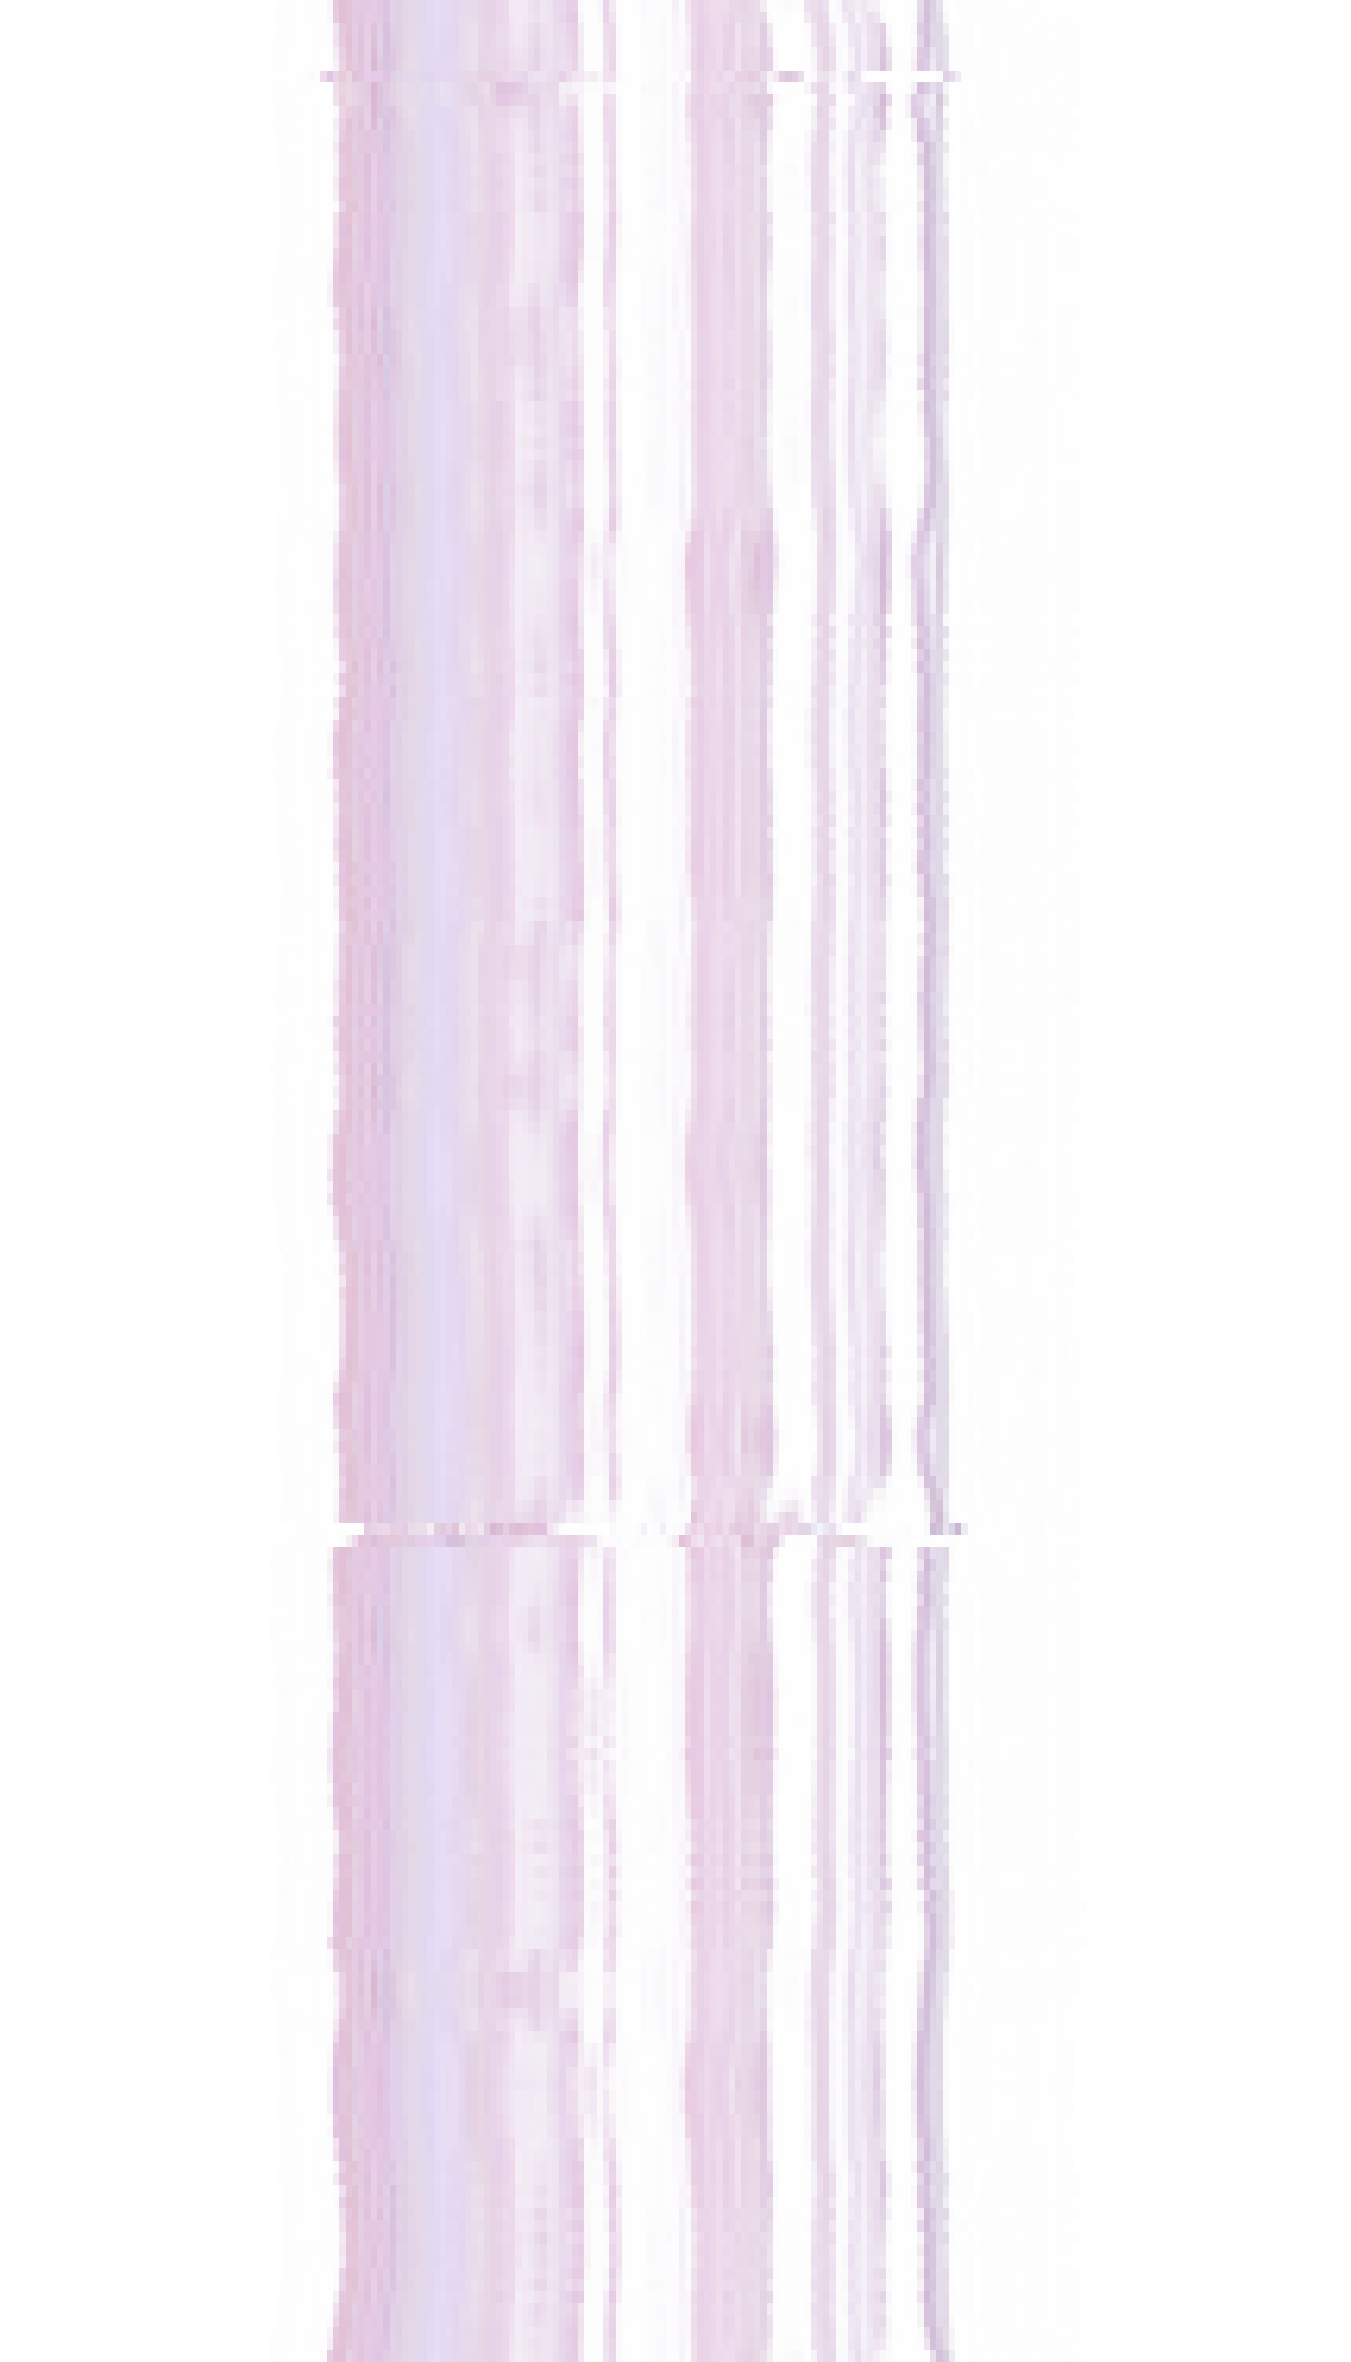
\includegraphics[height=0.33\textheight,type=pdf,ext=.pdf,read=.pdf]{Ch7/Figs/dummies/cross_section_200_alpha0.4_10_0_088}\label{fig:subfig4}}
    % filename format: cross_section_perfect_200_alpha0.4_DIMENSION_SLICE
    \subfigure[][without noise]{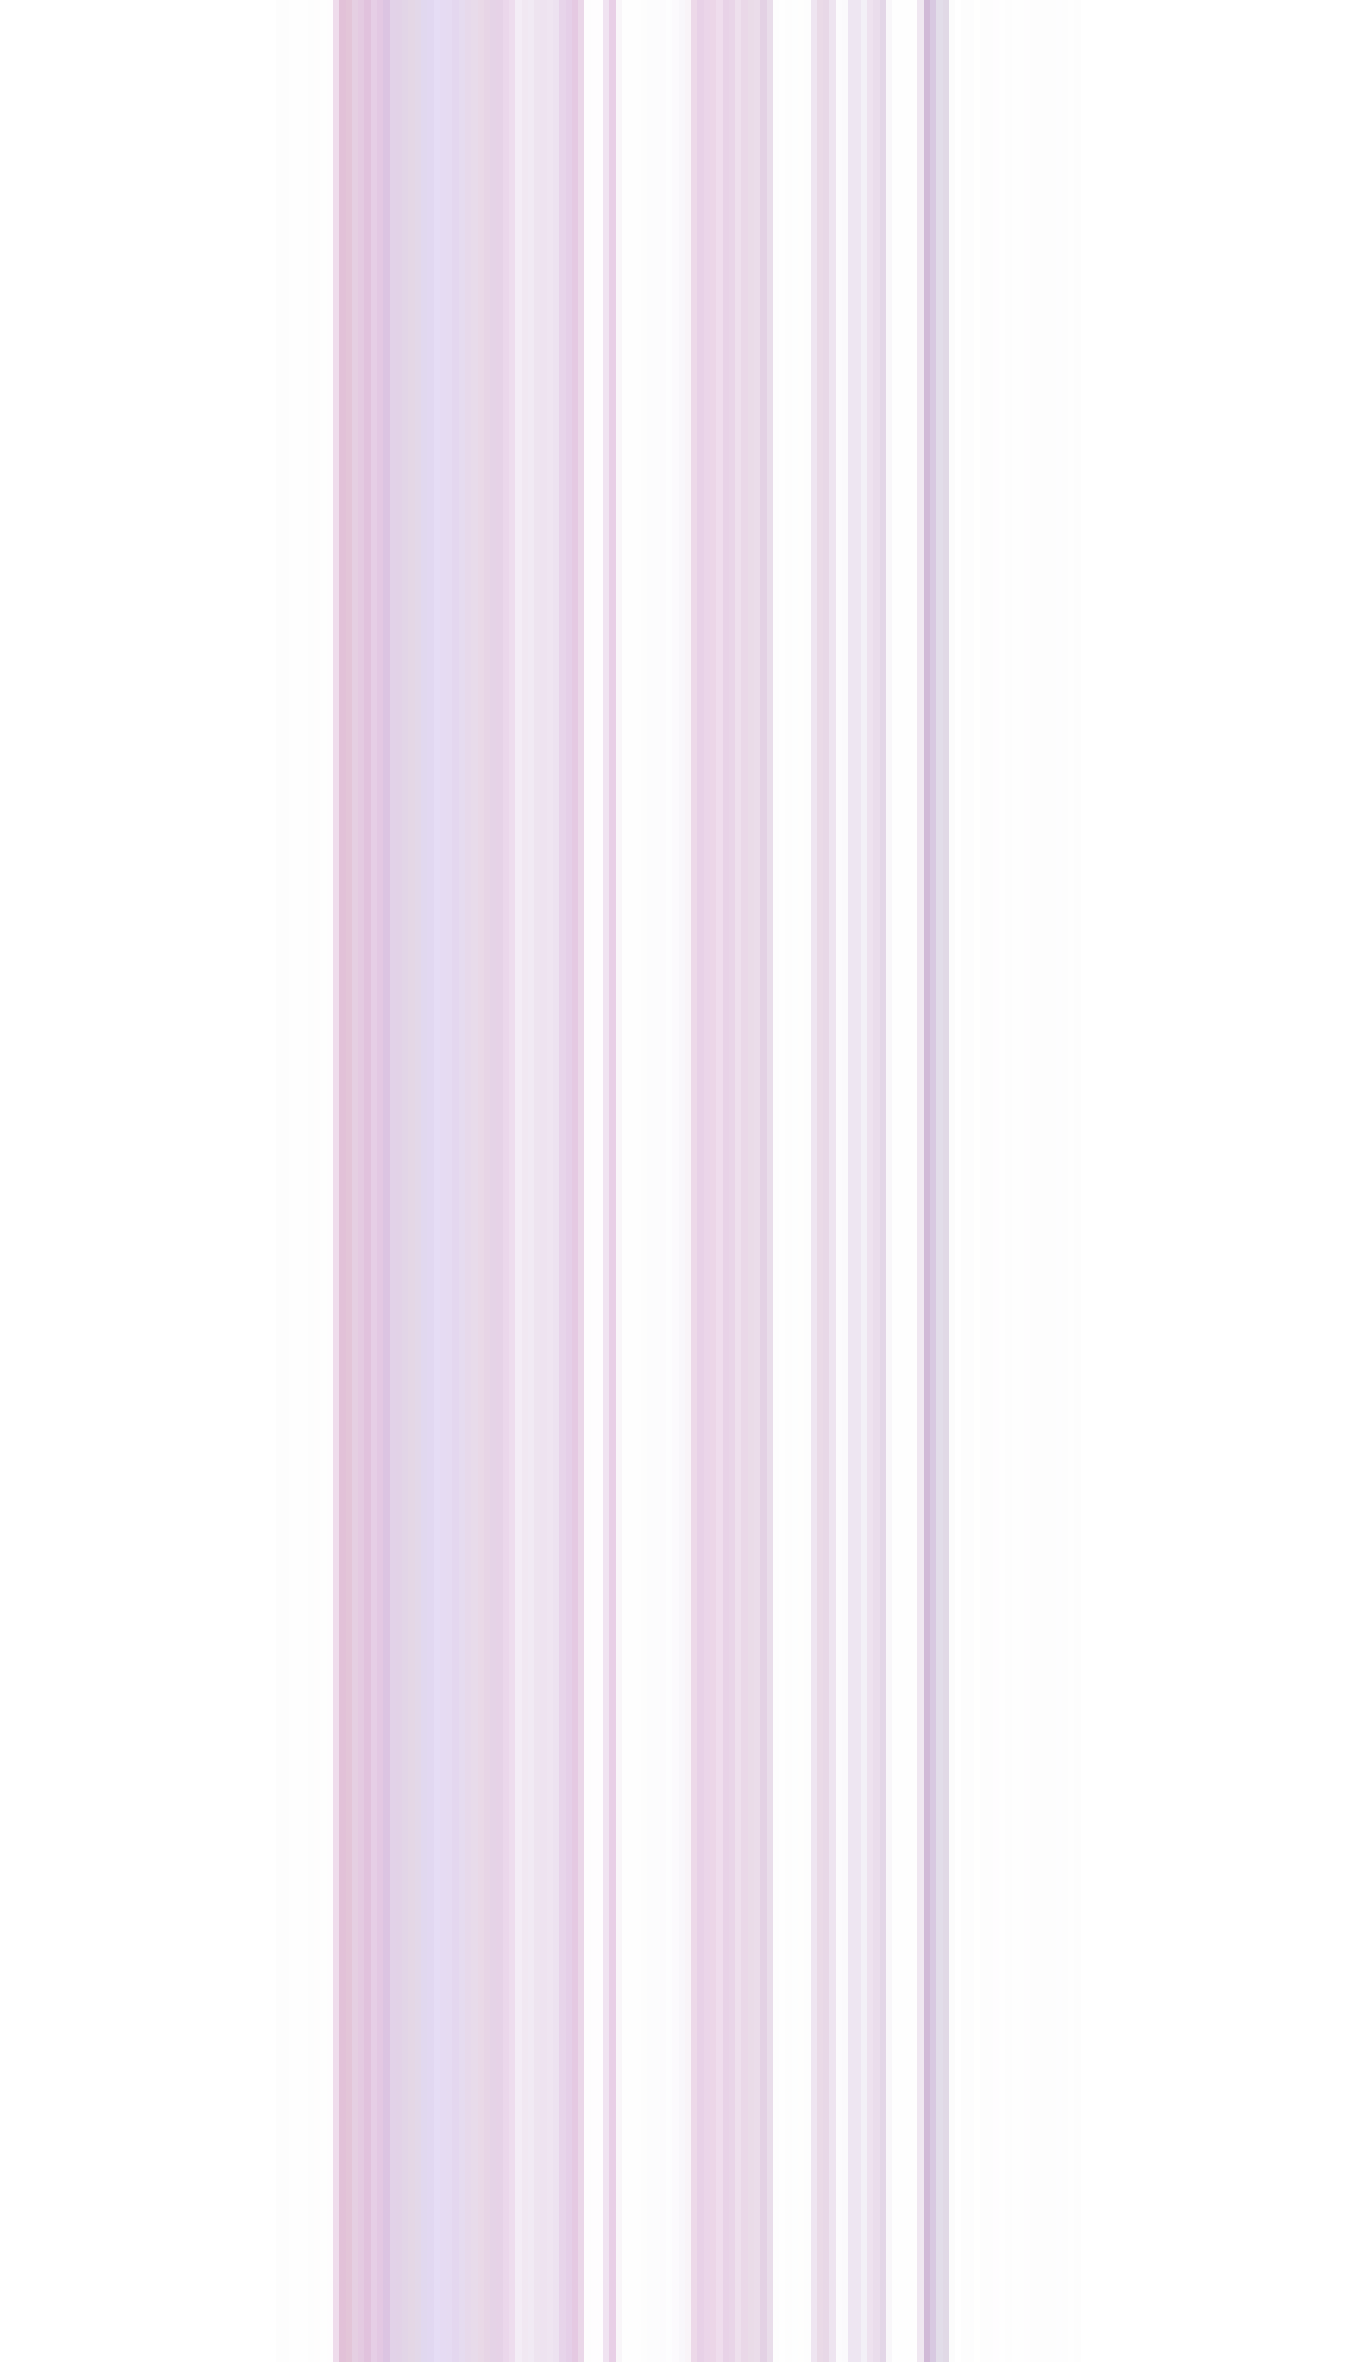
\includegraphics[height=0.33\textheight,type=pdf,ext=.pdf,read=.pdf]{Ch7/Figs/dummies/cross_section_perfect_200_alpha0.4_0_088}}
    \caption{What a nice figure! Caption of subfigures \subref{fig:subfig1}, \subref{fig:subfig2} and \subref{fig:subfig3}}
    \label{fig:dummy_cross_sections}
  \end{sidewaysfigure}
  
  \begin{sidewaysfigure}[htbp]
    \centering
    \subfigure[][0 iterations]{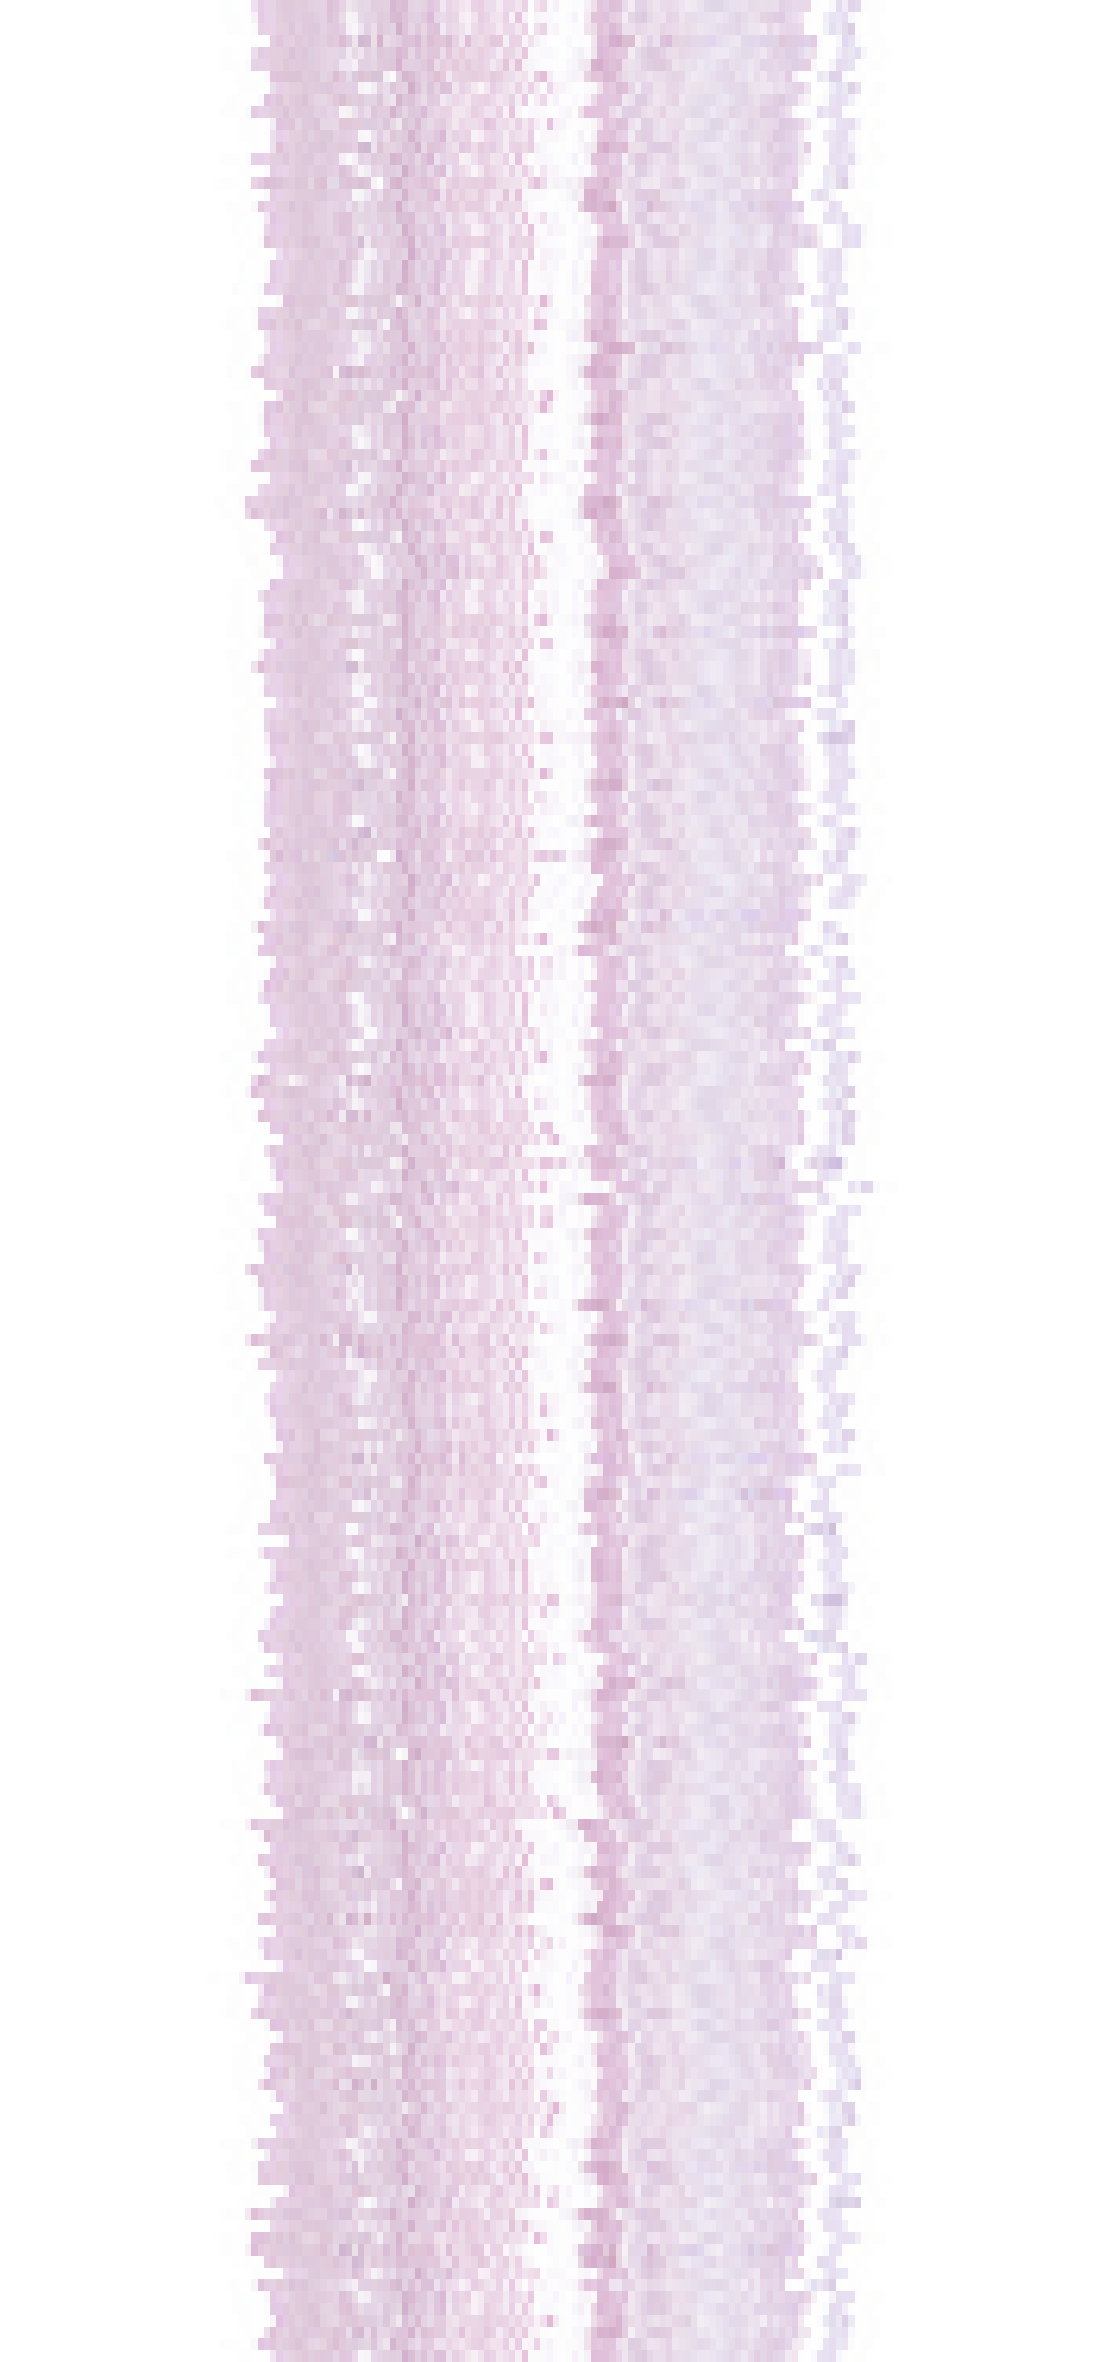
\includegraphics[height=0.33\textheight,type=pdf,ext=.pdf,read=.pdf]{Ch7/Figs/dummies/cross_section_200_alpha0.4_0_1_107}}
    \subfigure[][1 iteration]{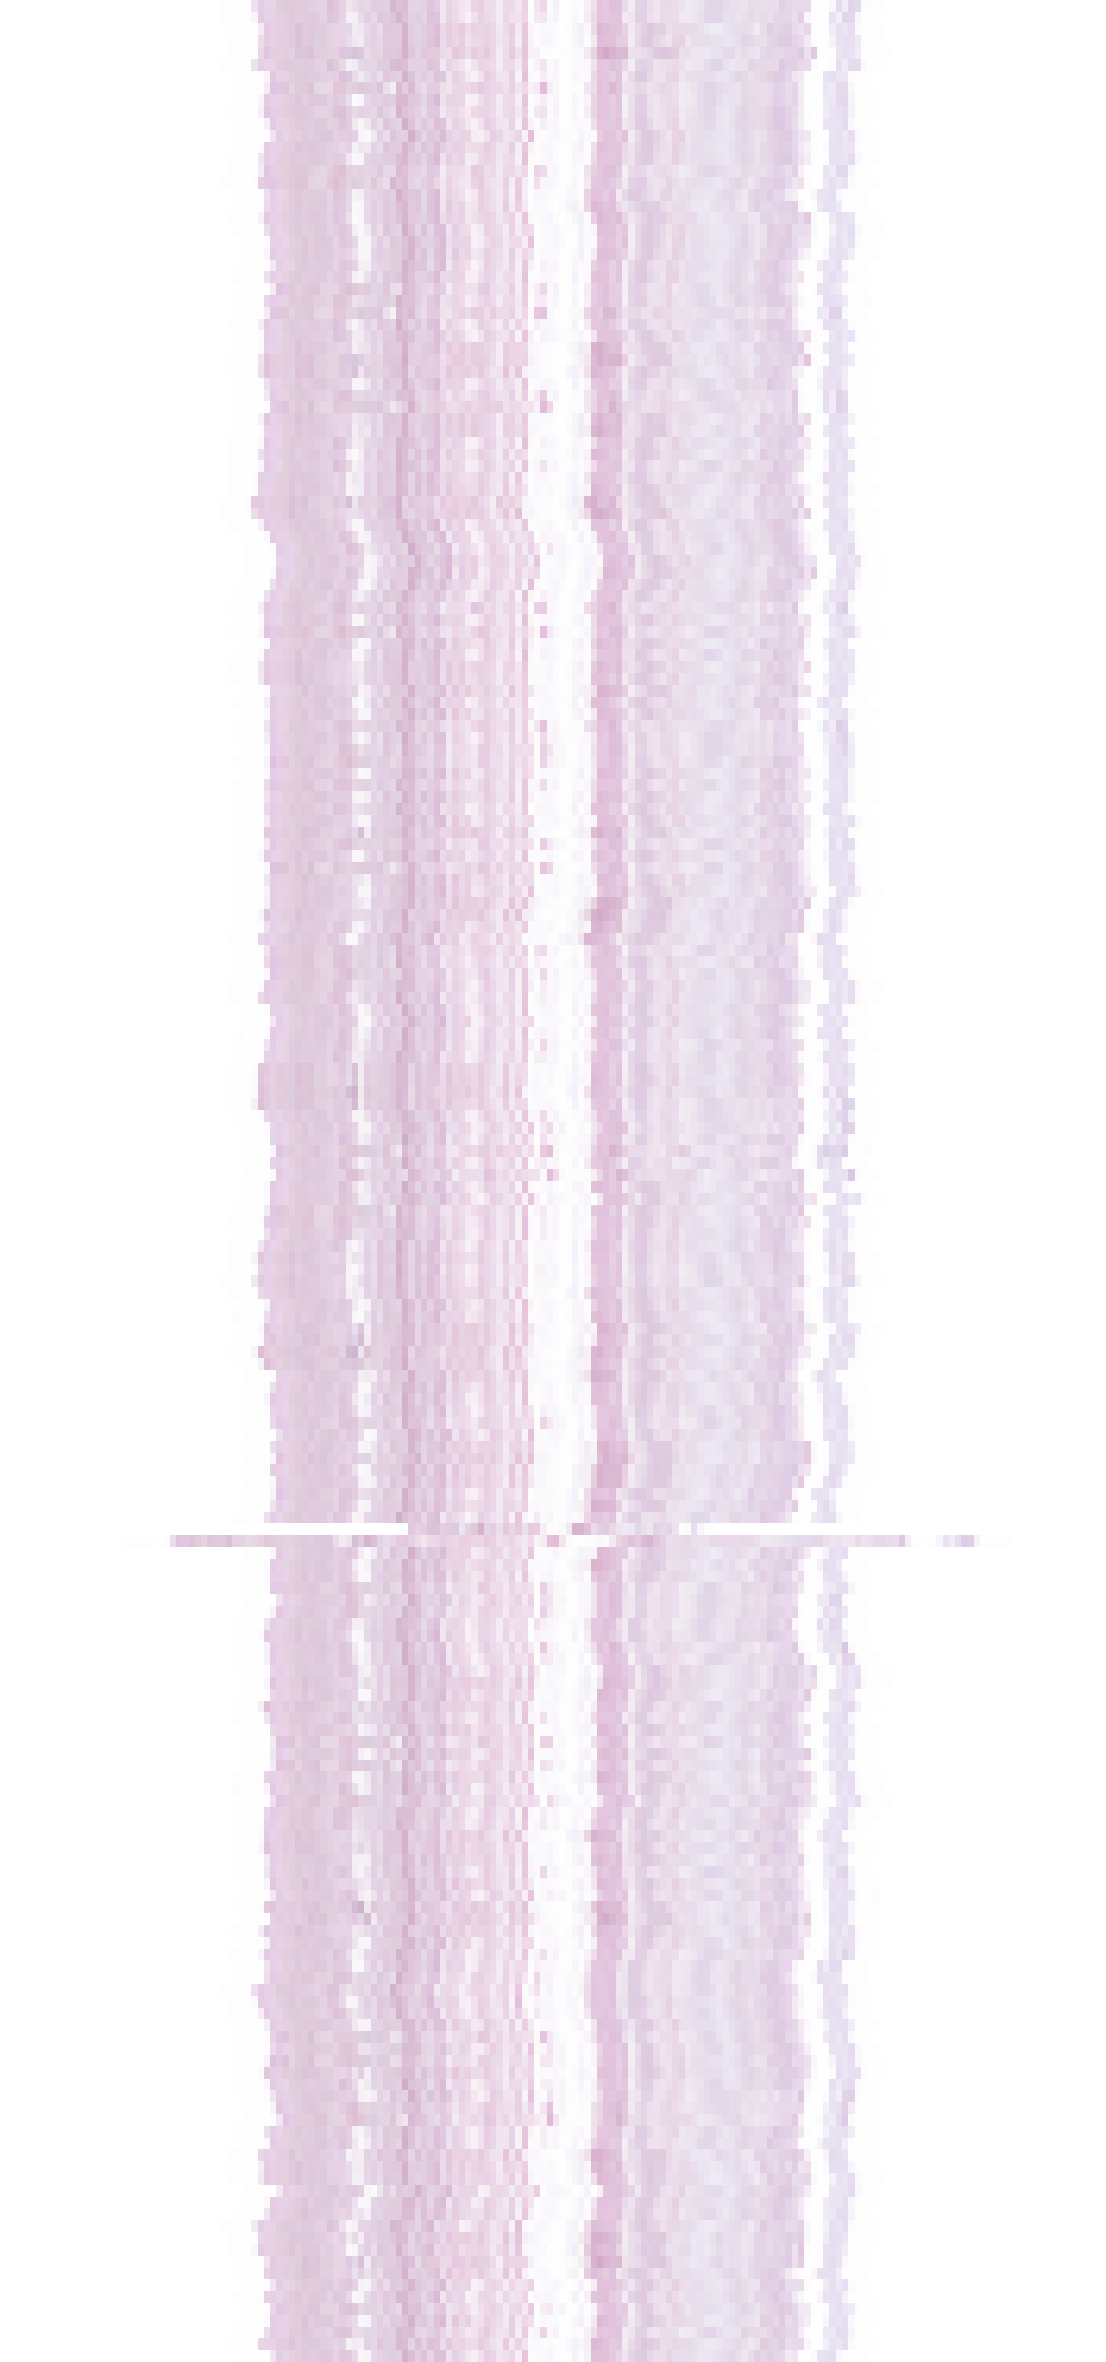
\includegraphics[height=0.33\textheight,type=pdf,ext=.pdf,read=.pdf]{Ch7/Figs/dummies/cross_section_200_alpha0.4_1_1_107}}
    \subfigure[][3 iterations]{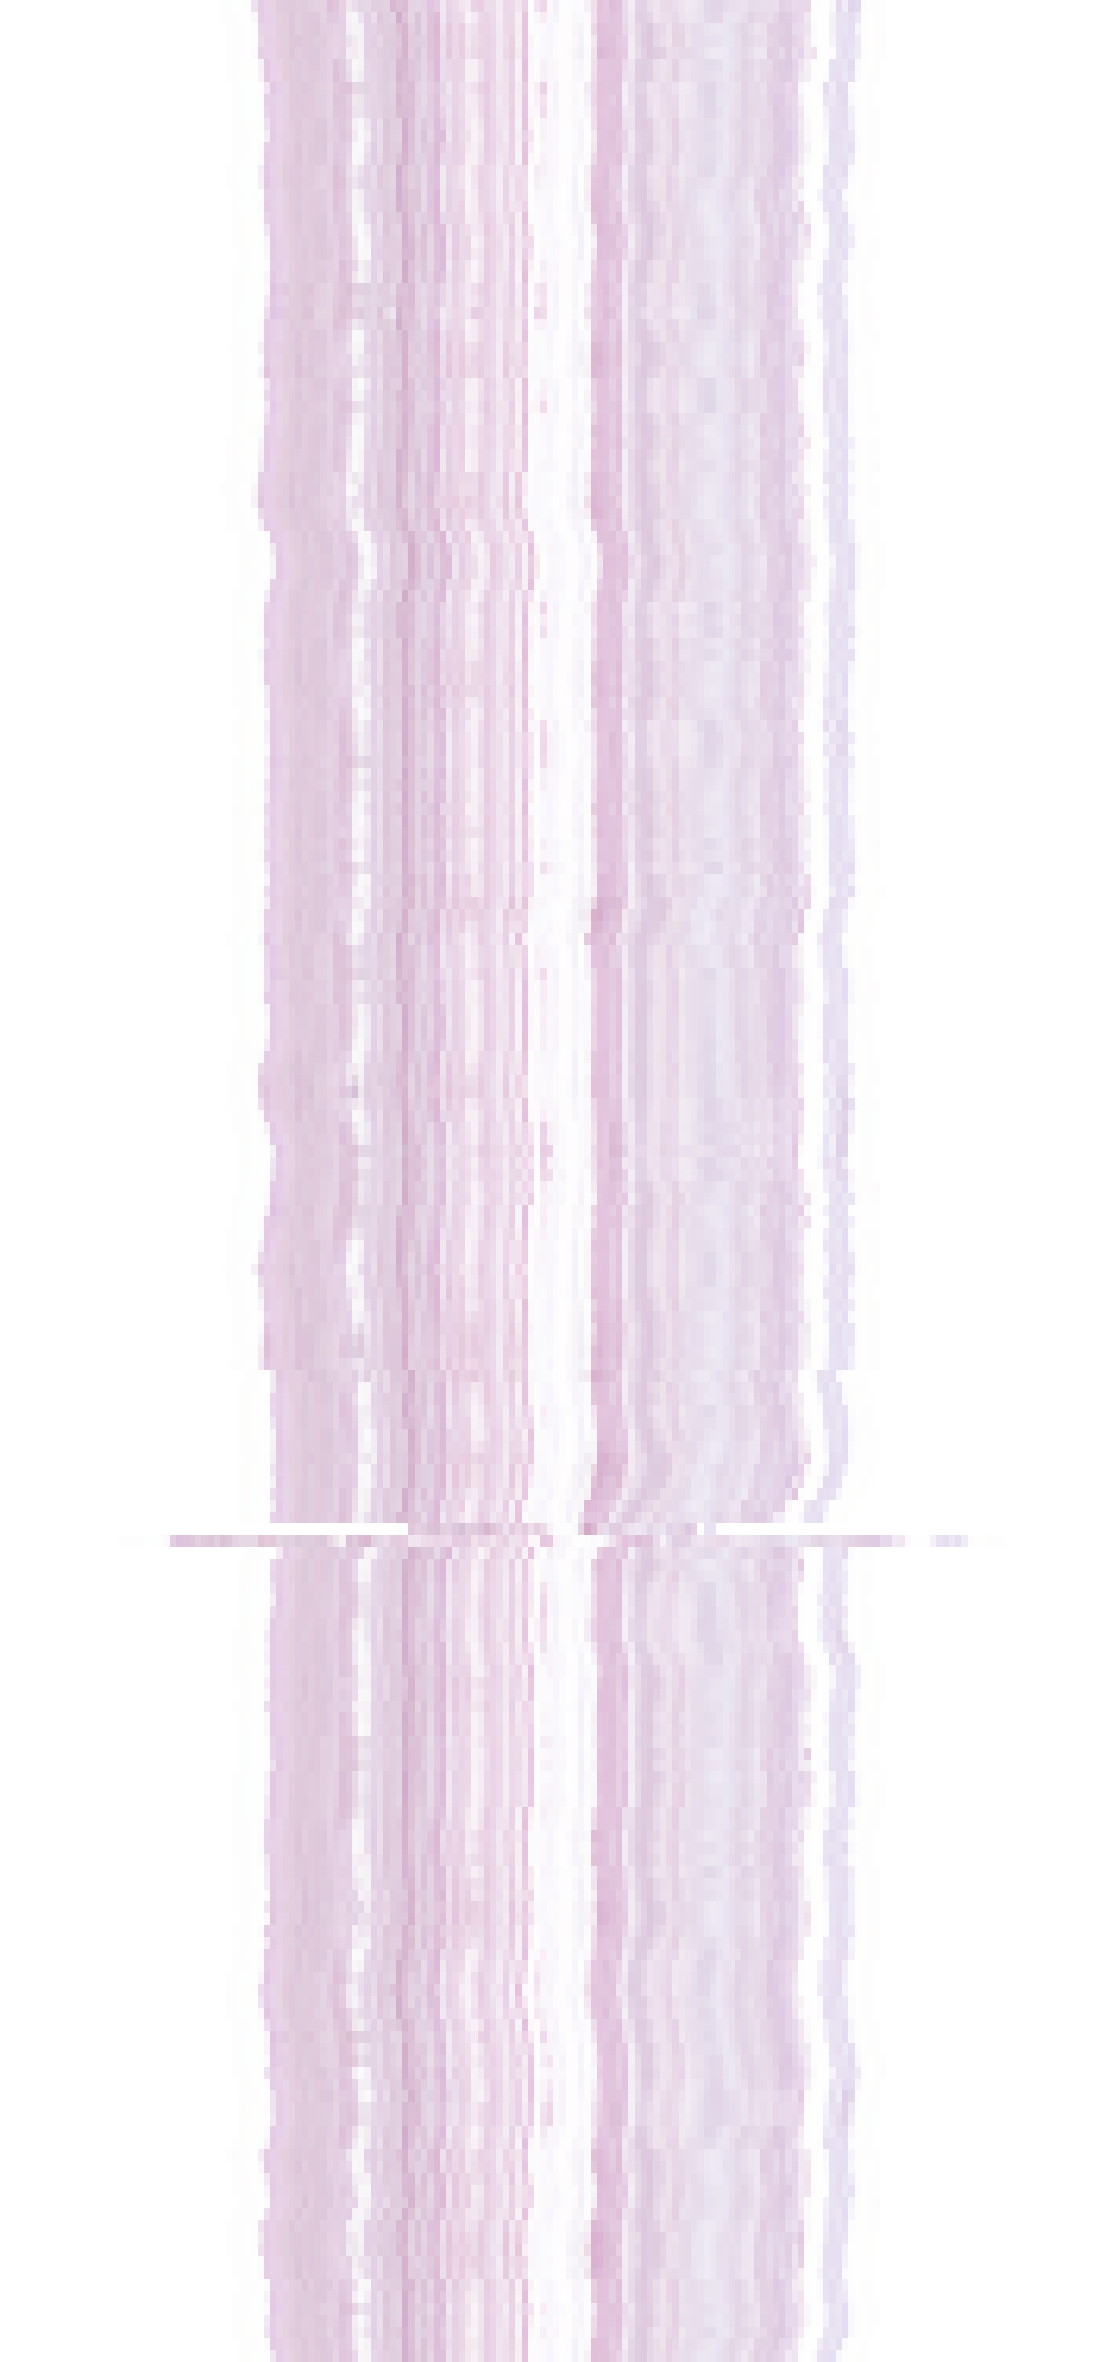
\includegraphics[height=0.33\textheight,type=pdf,ext=.pdf,read=.pdf]{Ch7/Figs/dummies/cross_section_200_alpha0.4_3_1_107}}
    \subfigure[][10 iterations]{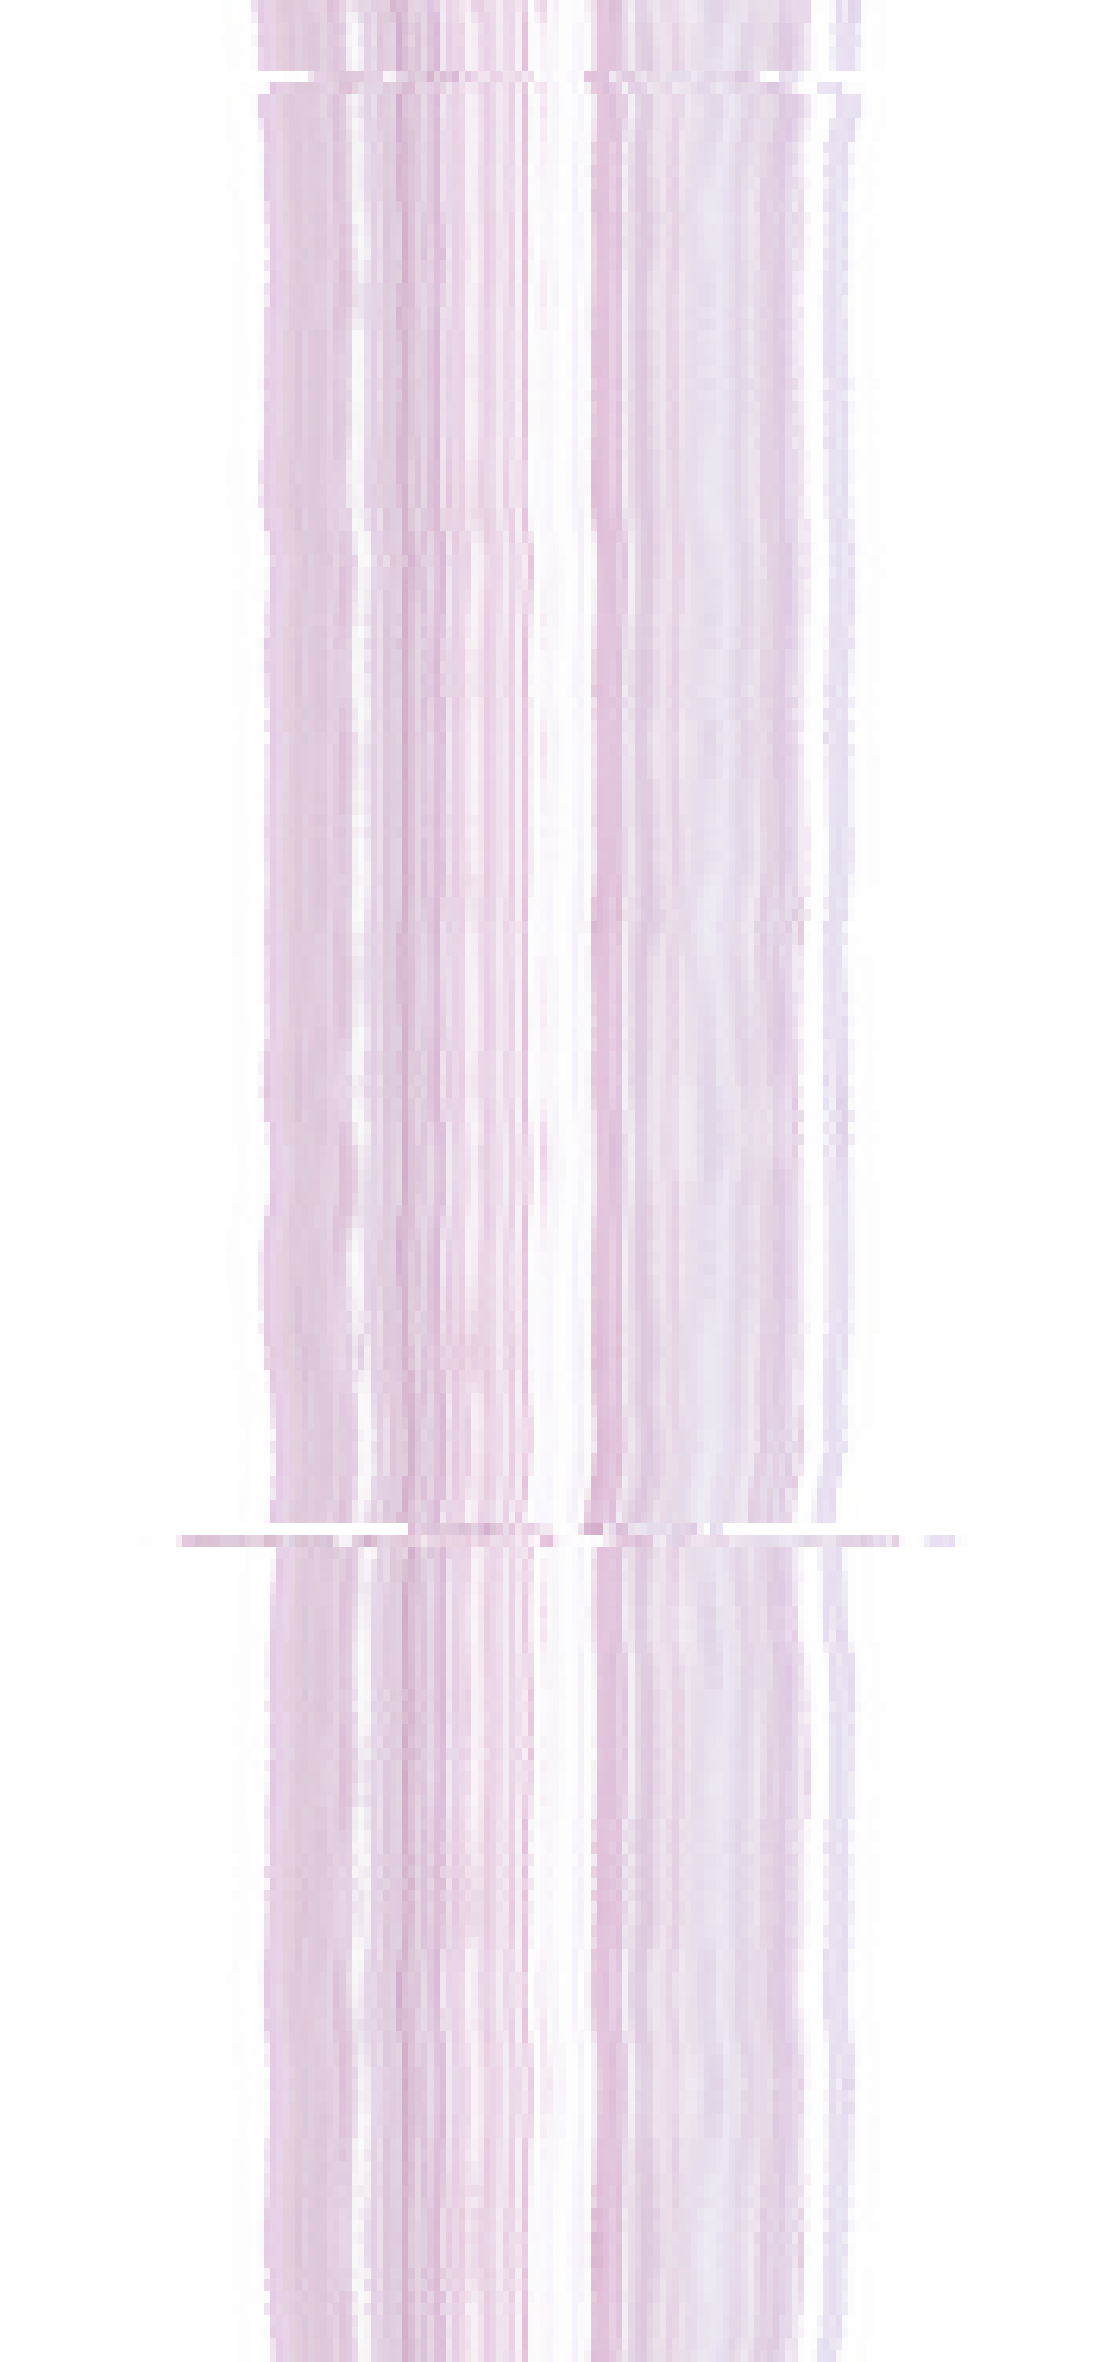
\includegraphics[height=0.33\textheight,type=pdf,ext=.pdf,read=.pdf]{Ch7/Figs/dummies/cross_section_200_alpha0.4_10_1_107}}
    \subfigure[][without noise]{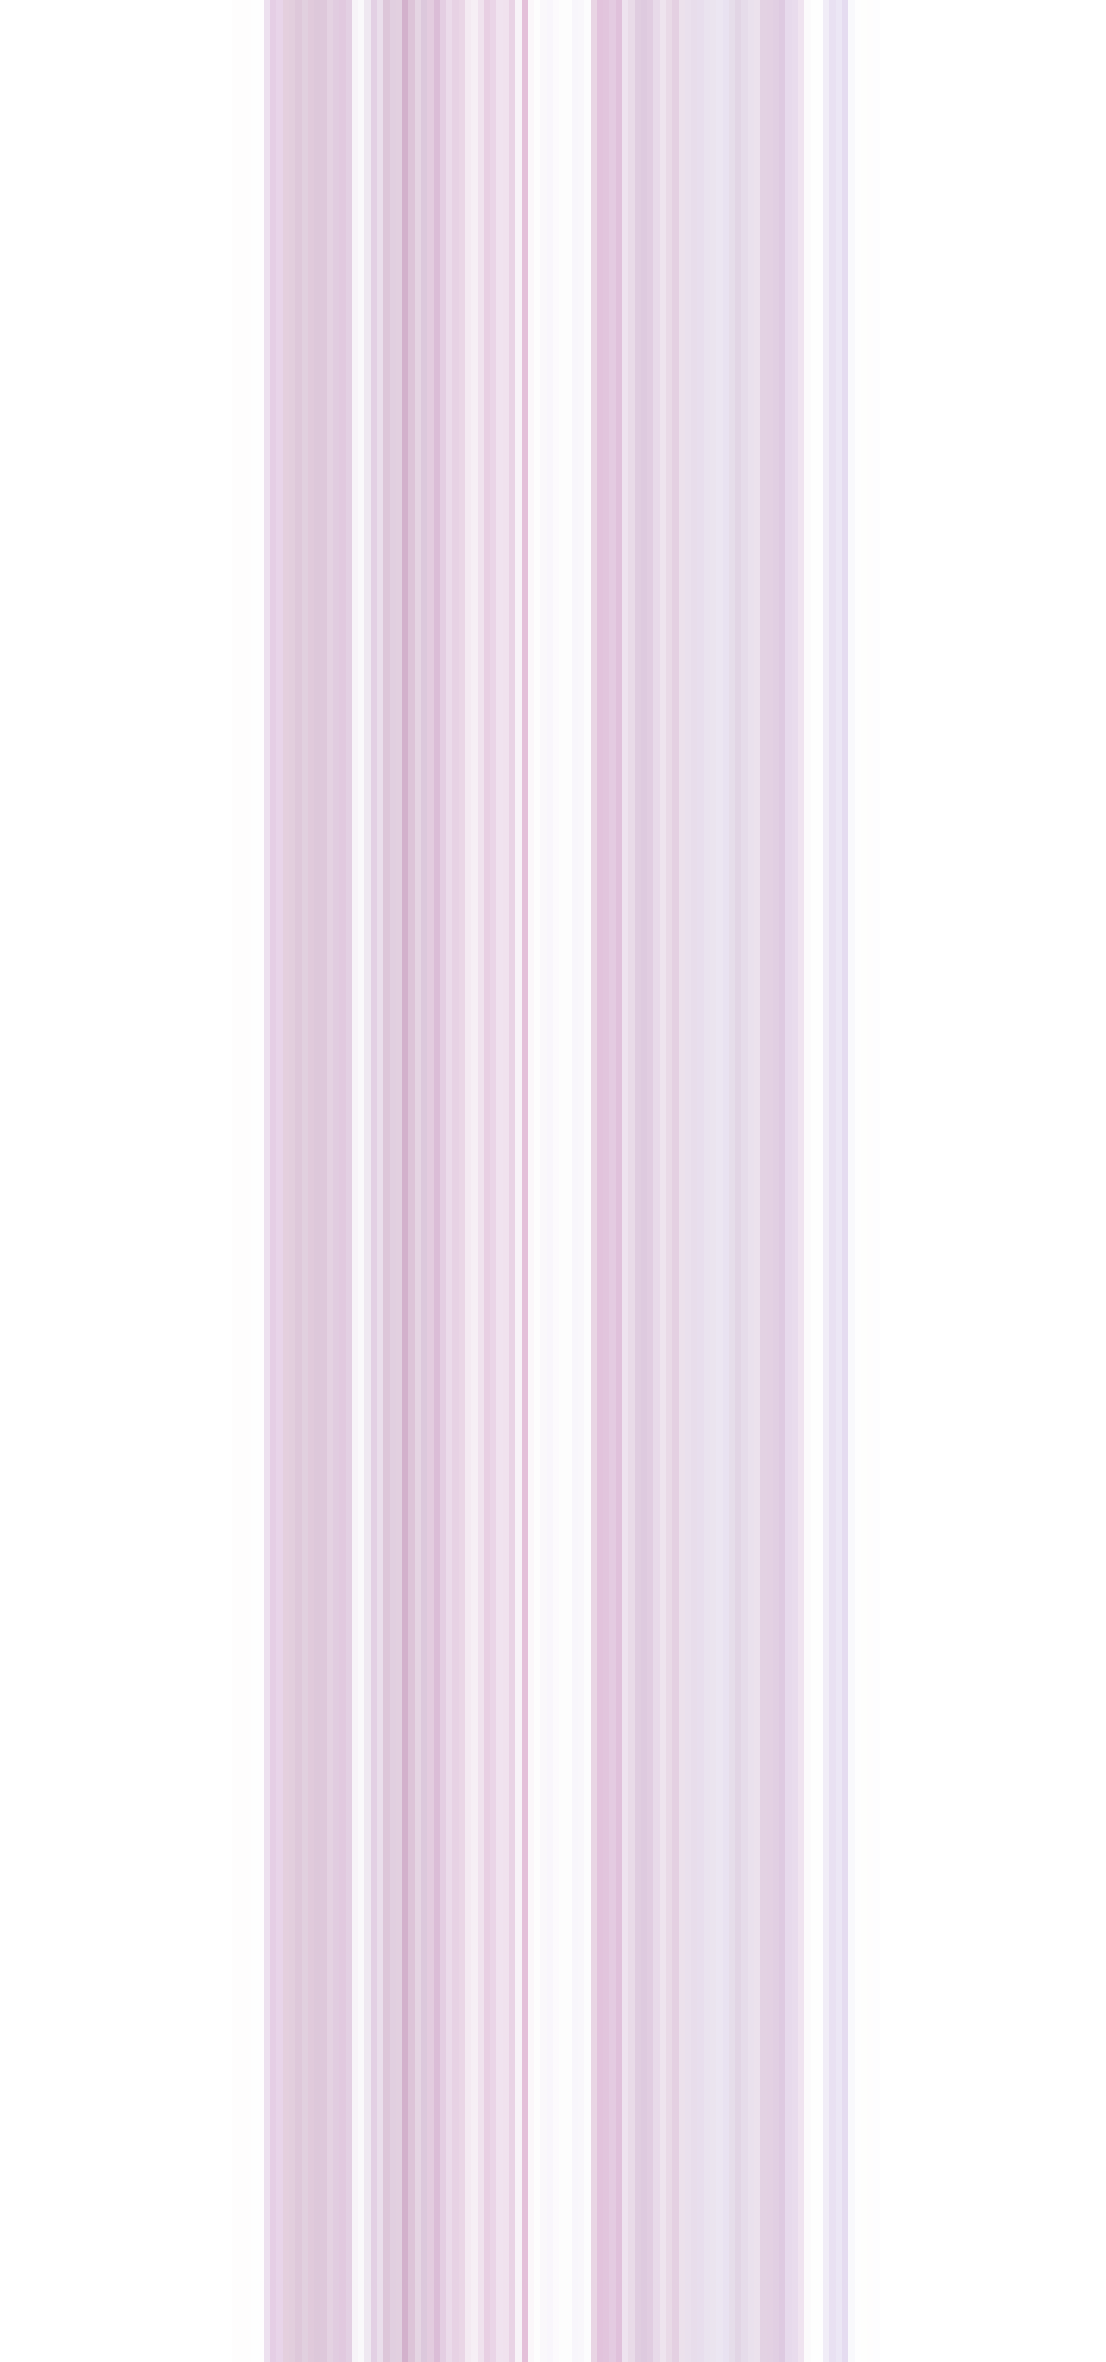
\includegraphics[height=0.33\textheight,type=pdf,ext=.pdf,read=.pdf]{Ch7/Figs/dummies/cross_section_perfect_200_alpha0.4_1_107}}
    \caption{What a nice figure!}
    \label{fig:dummy_cross_sections}
  \end{sidewaysfigure}
    
  % rotated
  \begin{sidewaysfigure}[htbp]
    \centering
    \subfigure[][0 iterations]{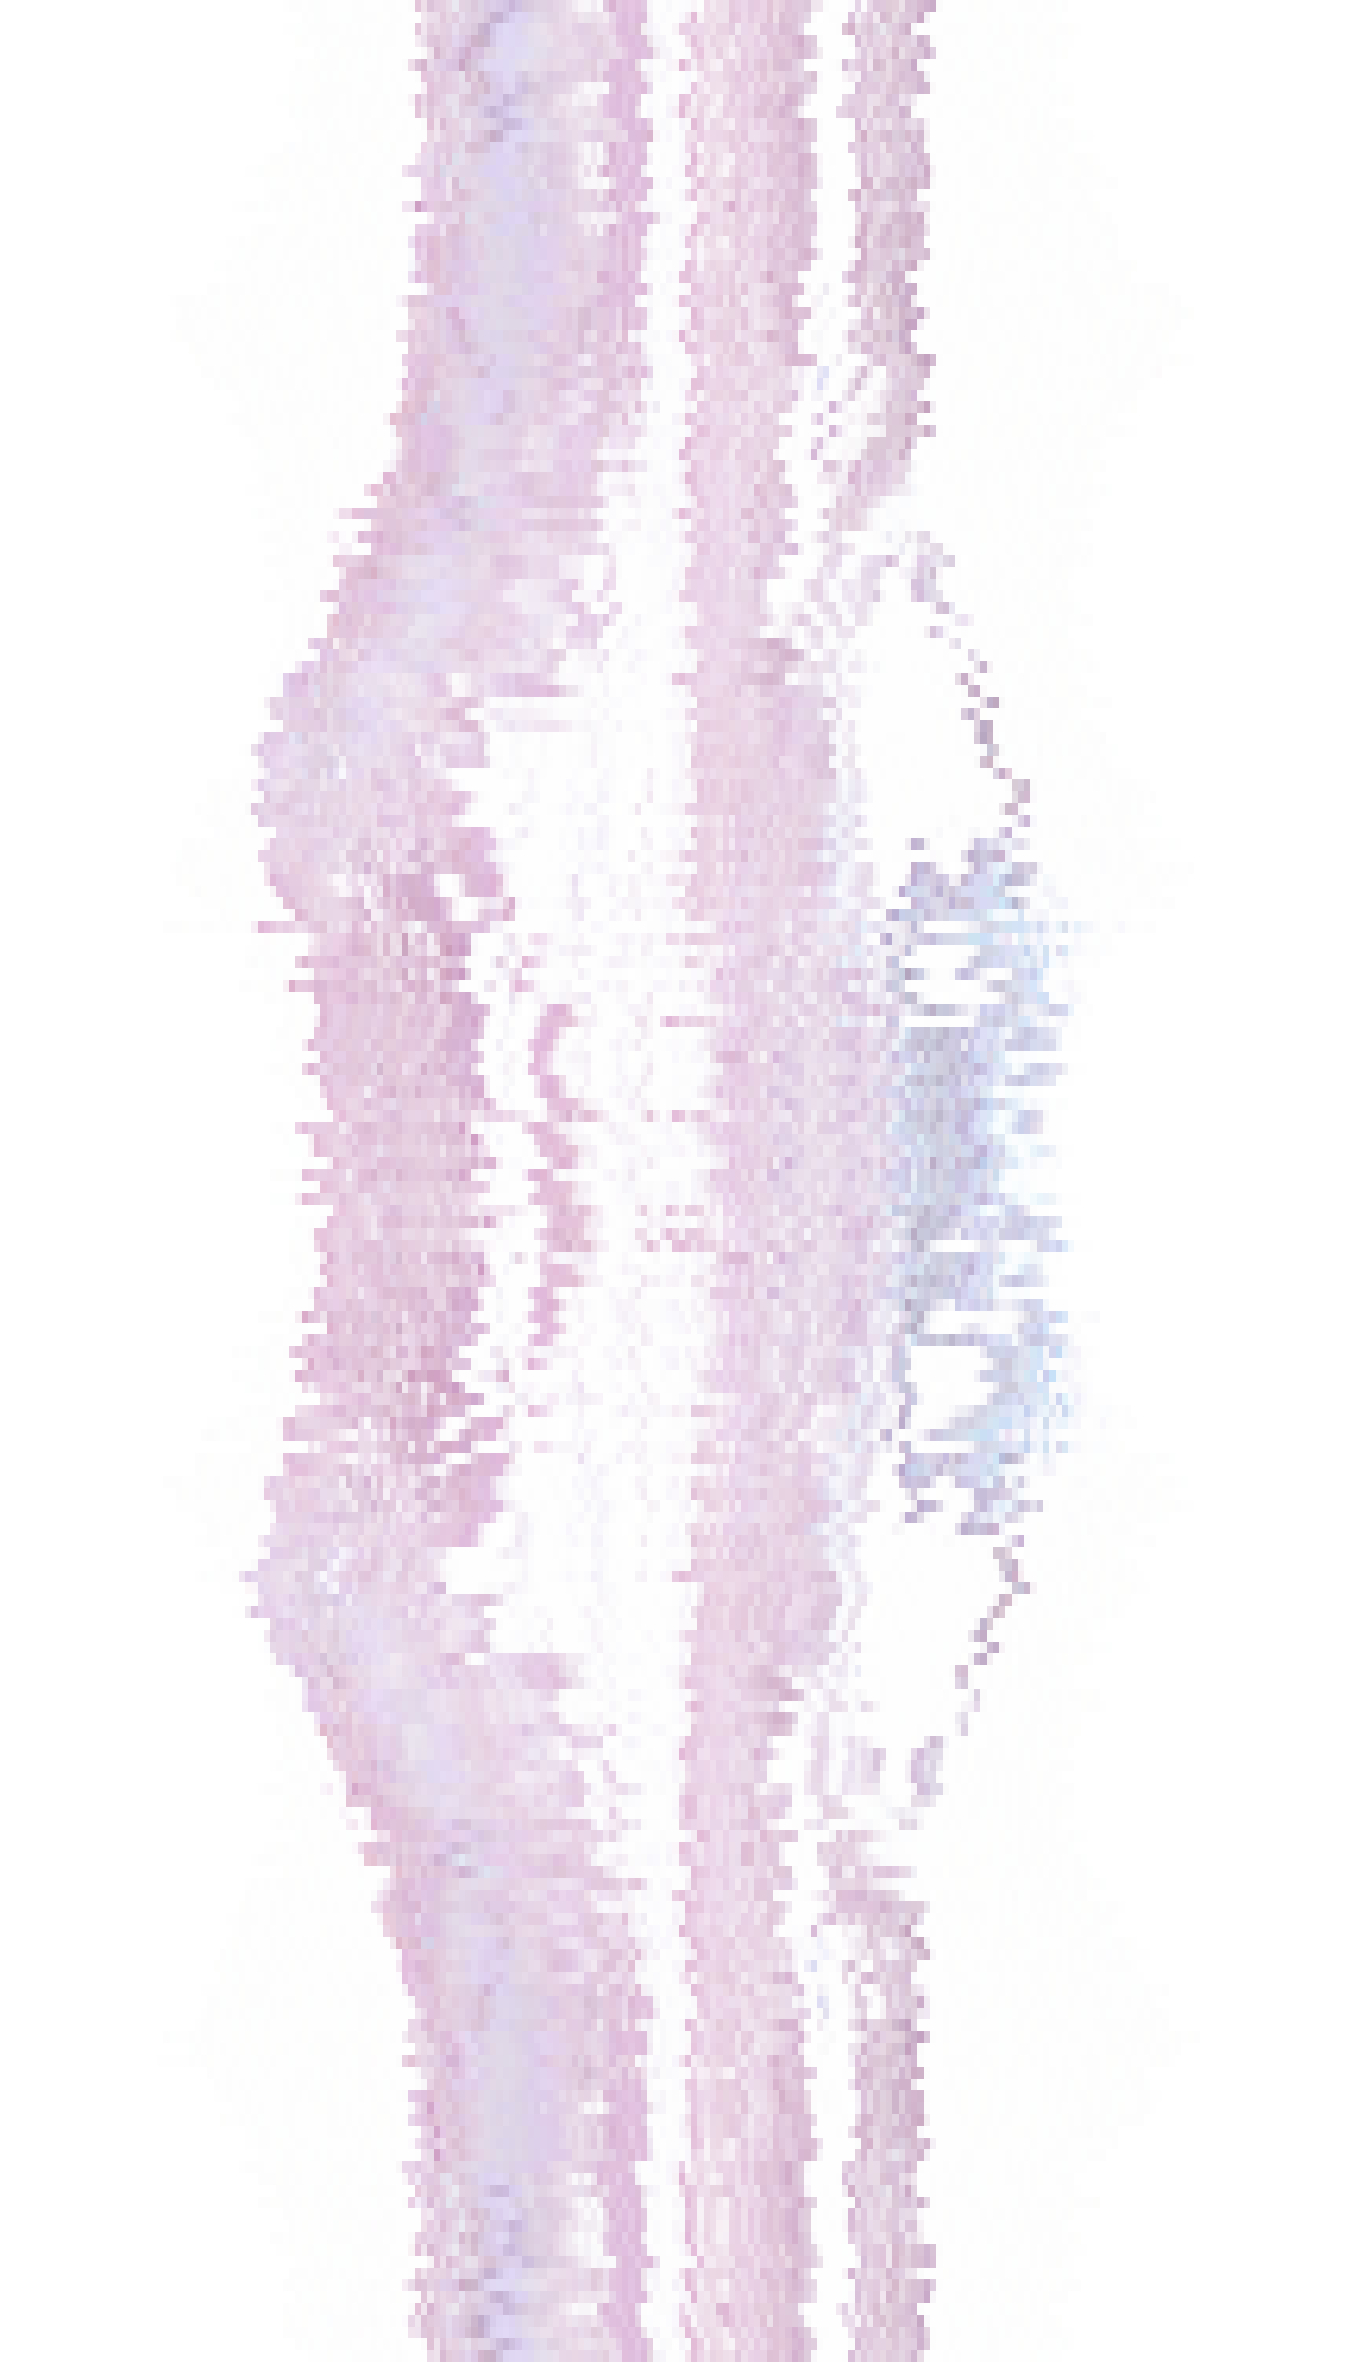
\includegraphics[height=0.33\textheight,type=pdf,ext=.pdf,read=.pdf]{Ch7/Figs/dummies/cross_section_200_alpha0.4r_0_0_088}}
    \subfigure[][1 iteration]{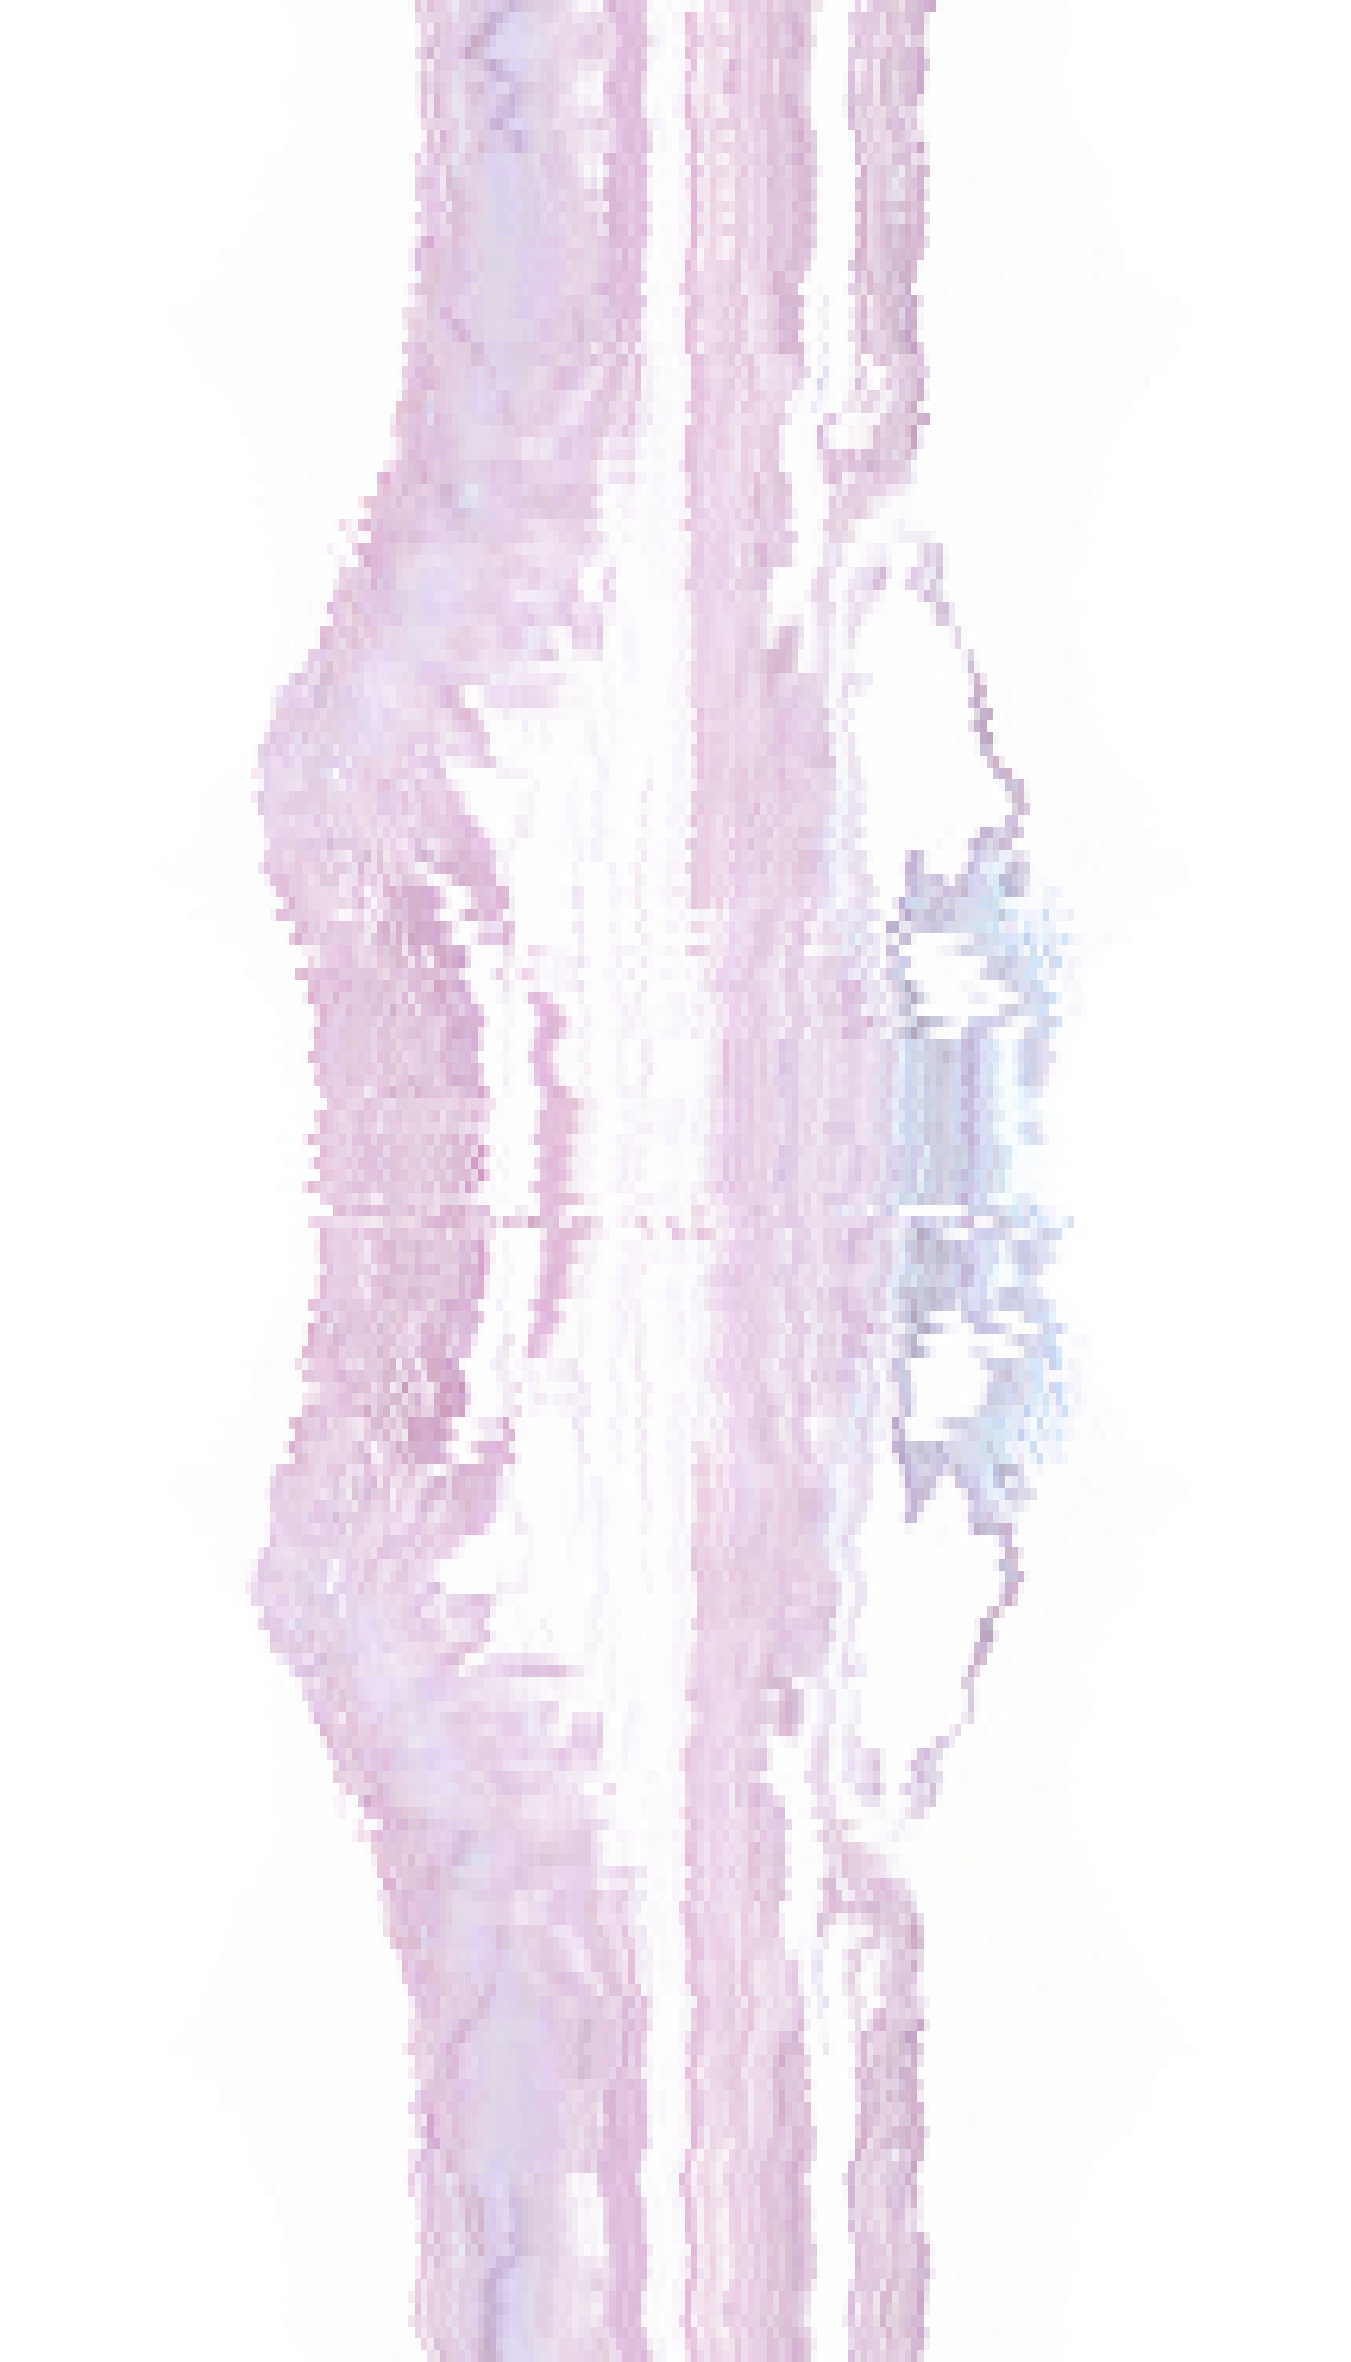
\includegraphics[height=0.33\textheight,type=pdf,ext=.pdf,read=.pdf]{Ch7/Figs/dummies/cross_section_200_alpha0.4r_1_0_088}}
    \subfigure[][3 iterations]{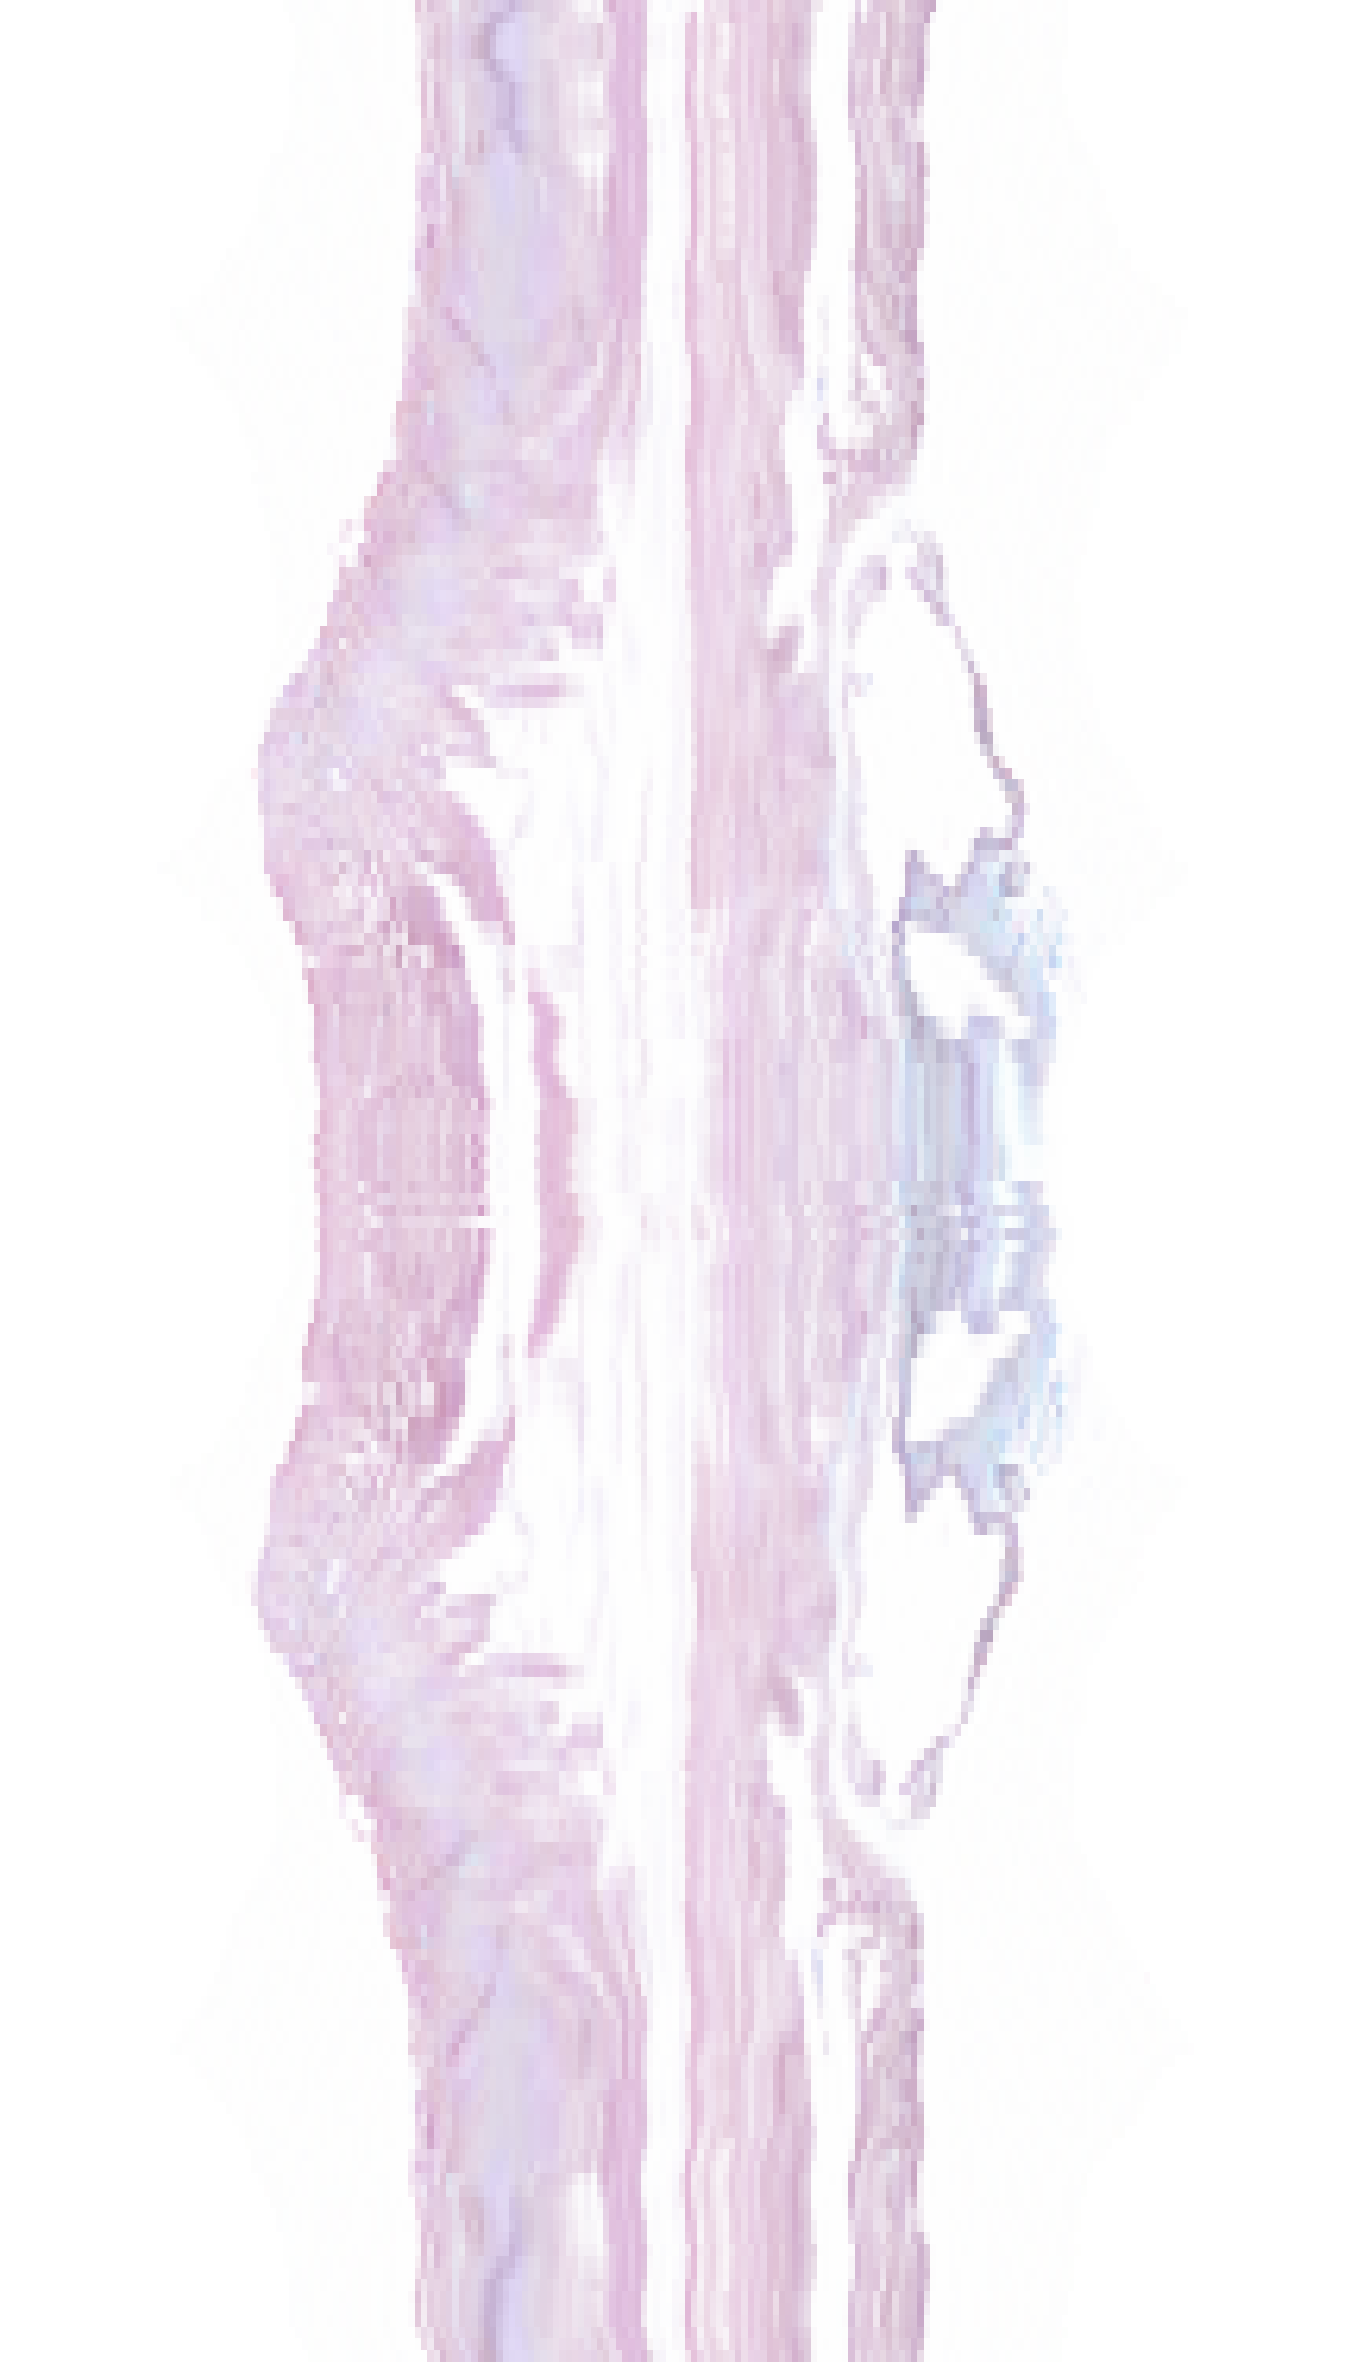
\includegraphics[height=0.33\textheight,type=pdf,ext=.pdf,read=.pdf]{Ch7/Figs/dummies/cross_section_200_alpha0.4r_3_0_088}}
    \subfigure[][10 iterations]{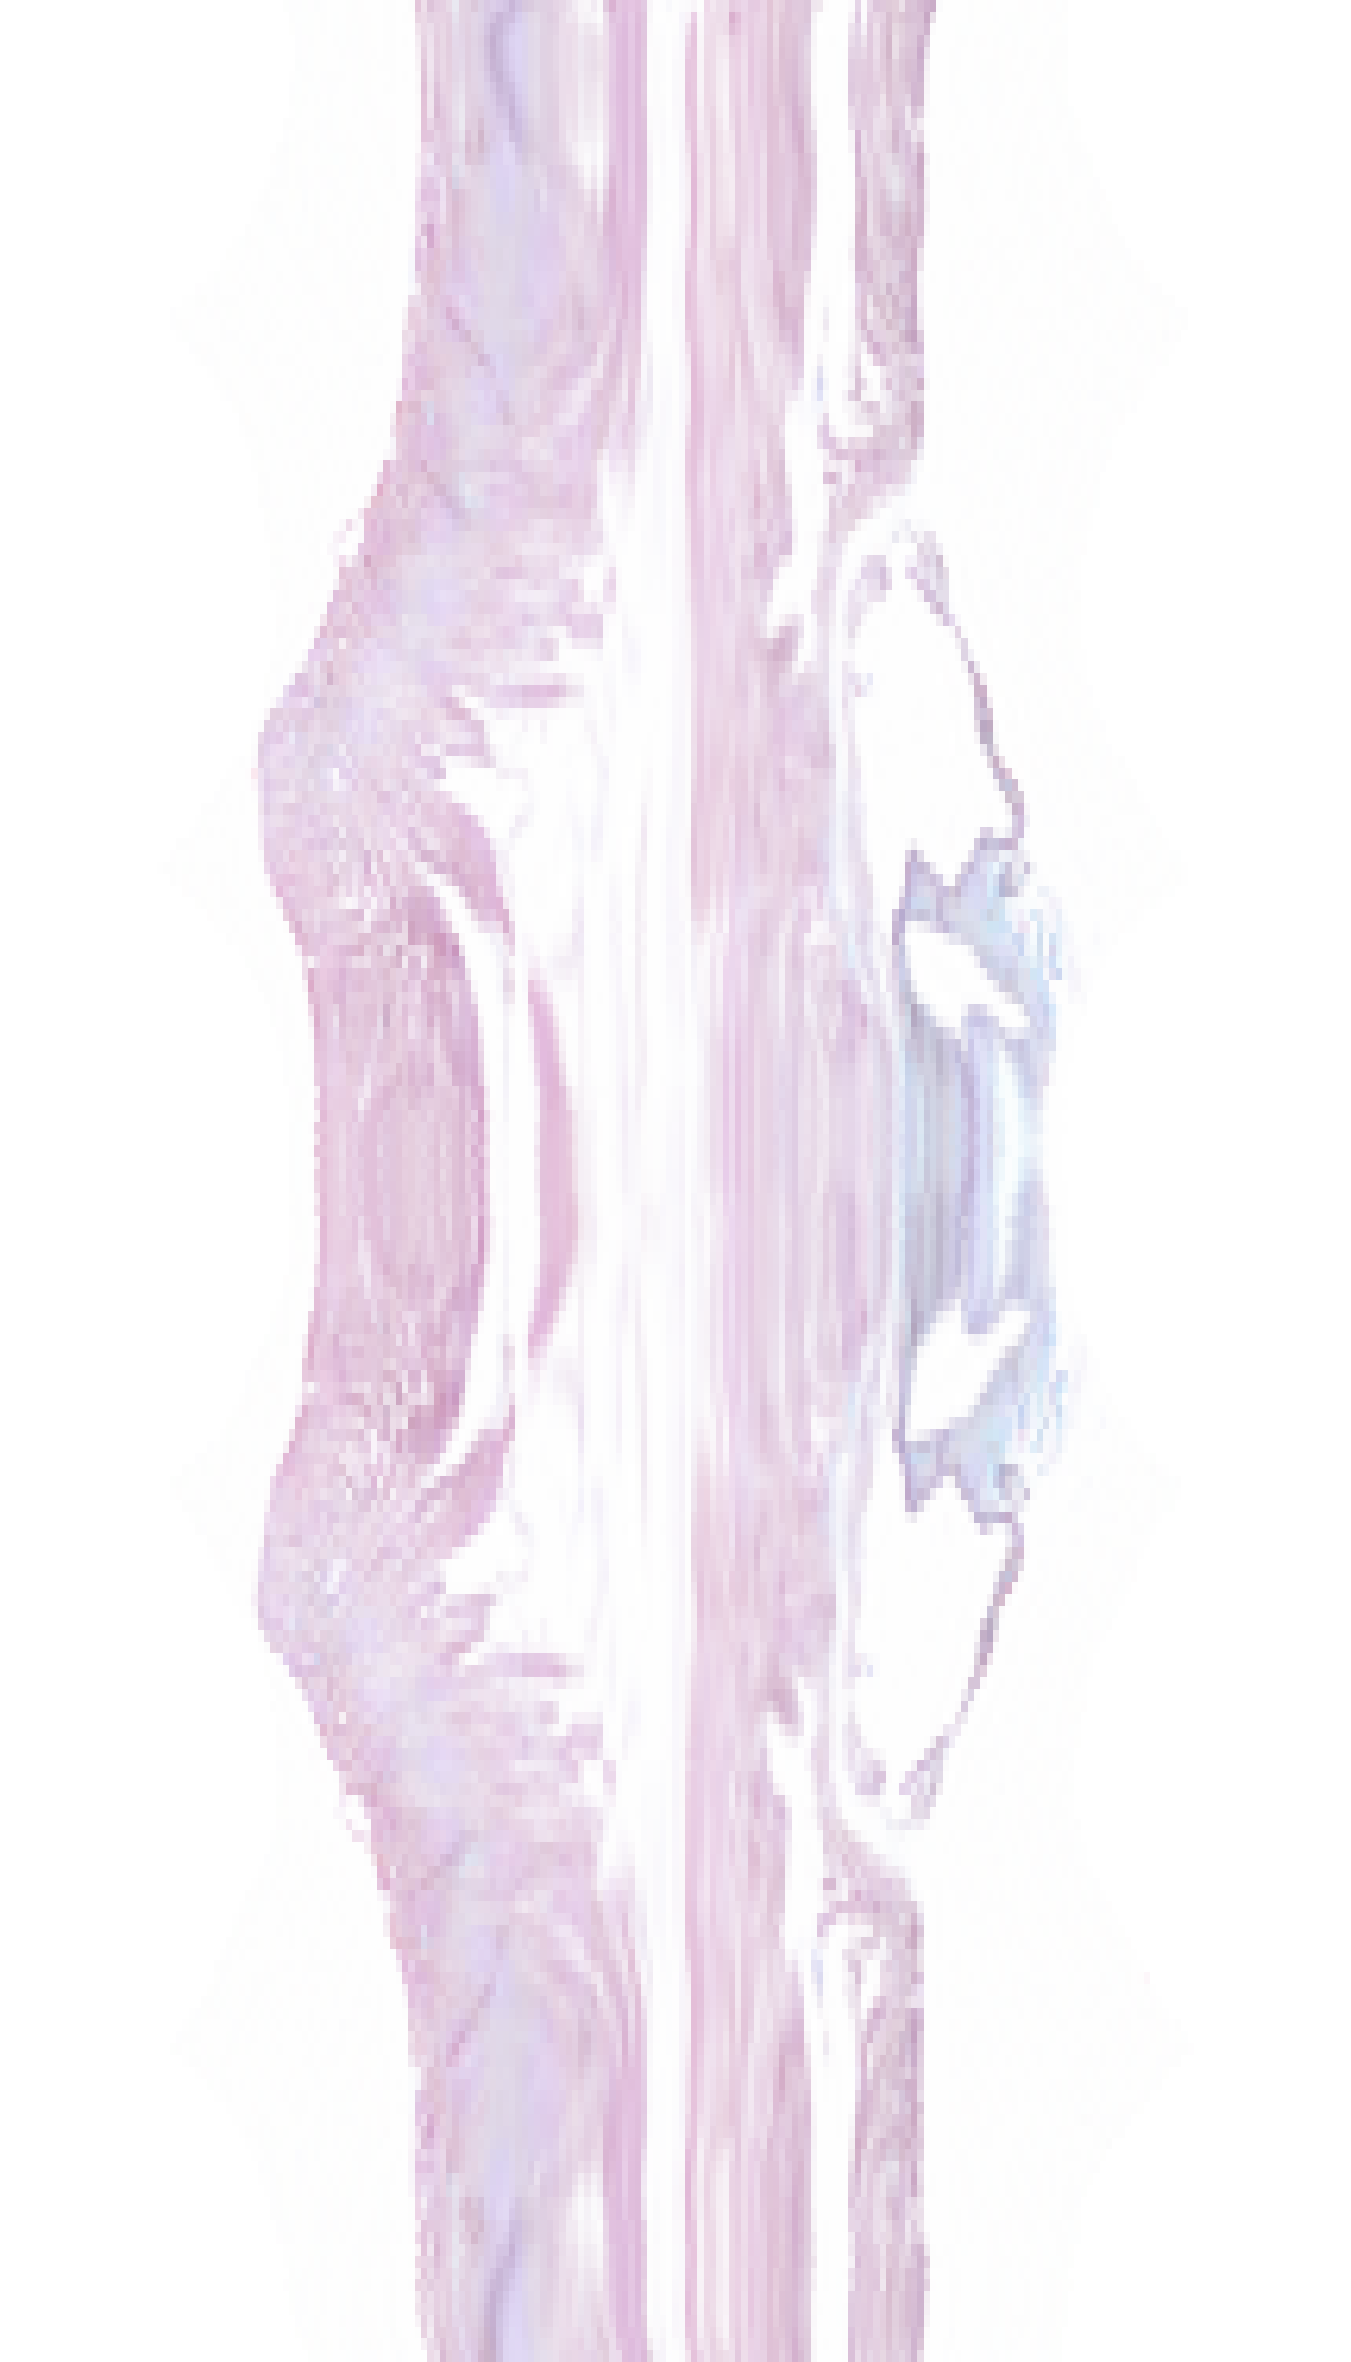
\includegraphics[height=0.33\textheight,type=pdf,ext=.pdf,read=.pdf]{Ch7/Figs/dummies/cross_section_200_alpha0.4r_10_0_088}}
    \subfigure[][without noise]{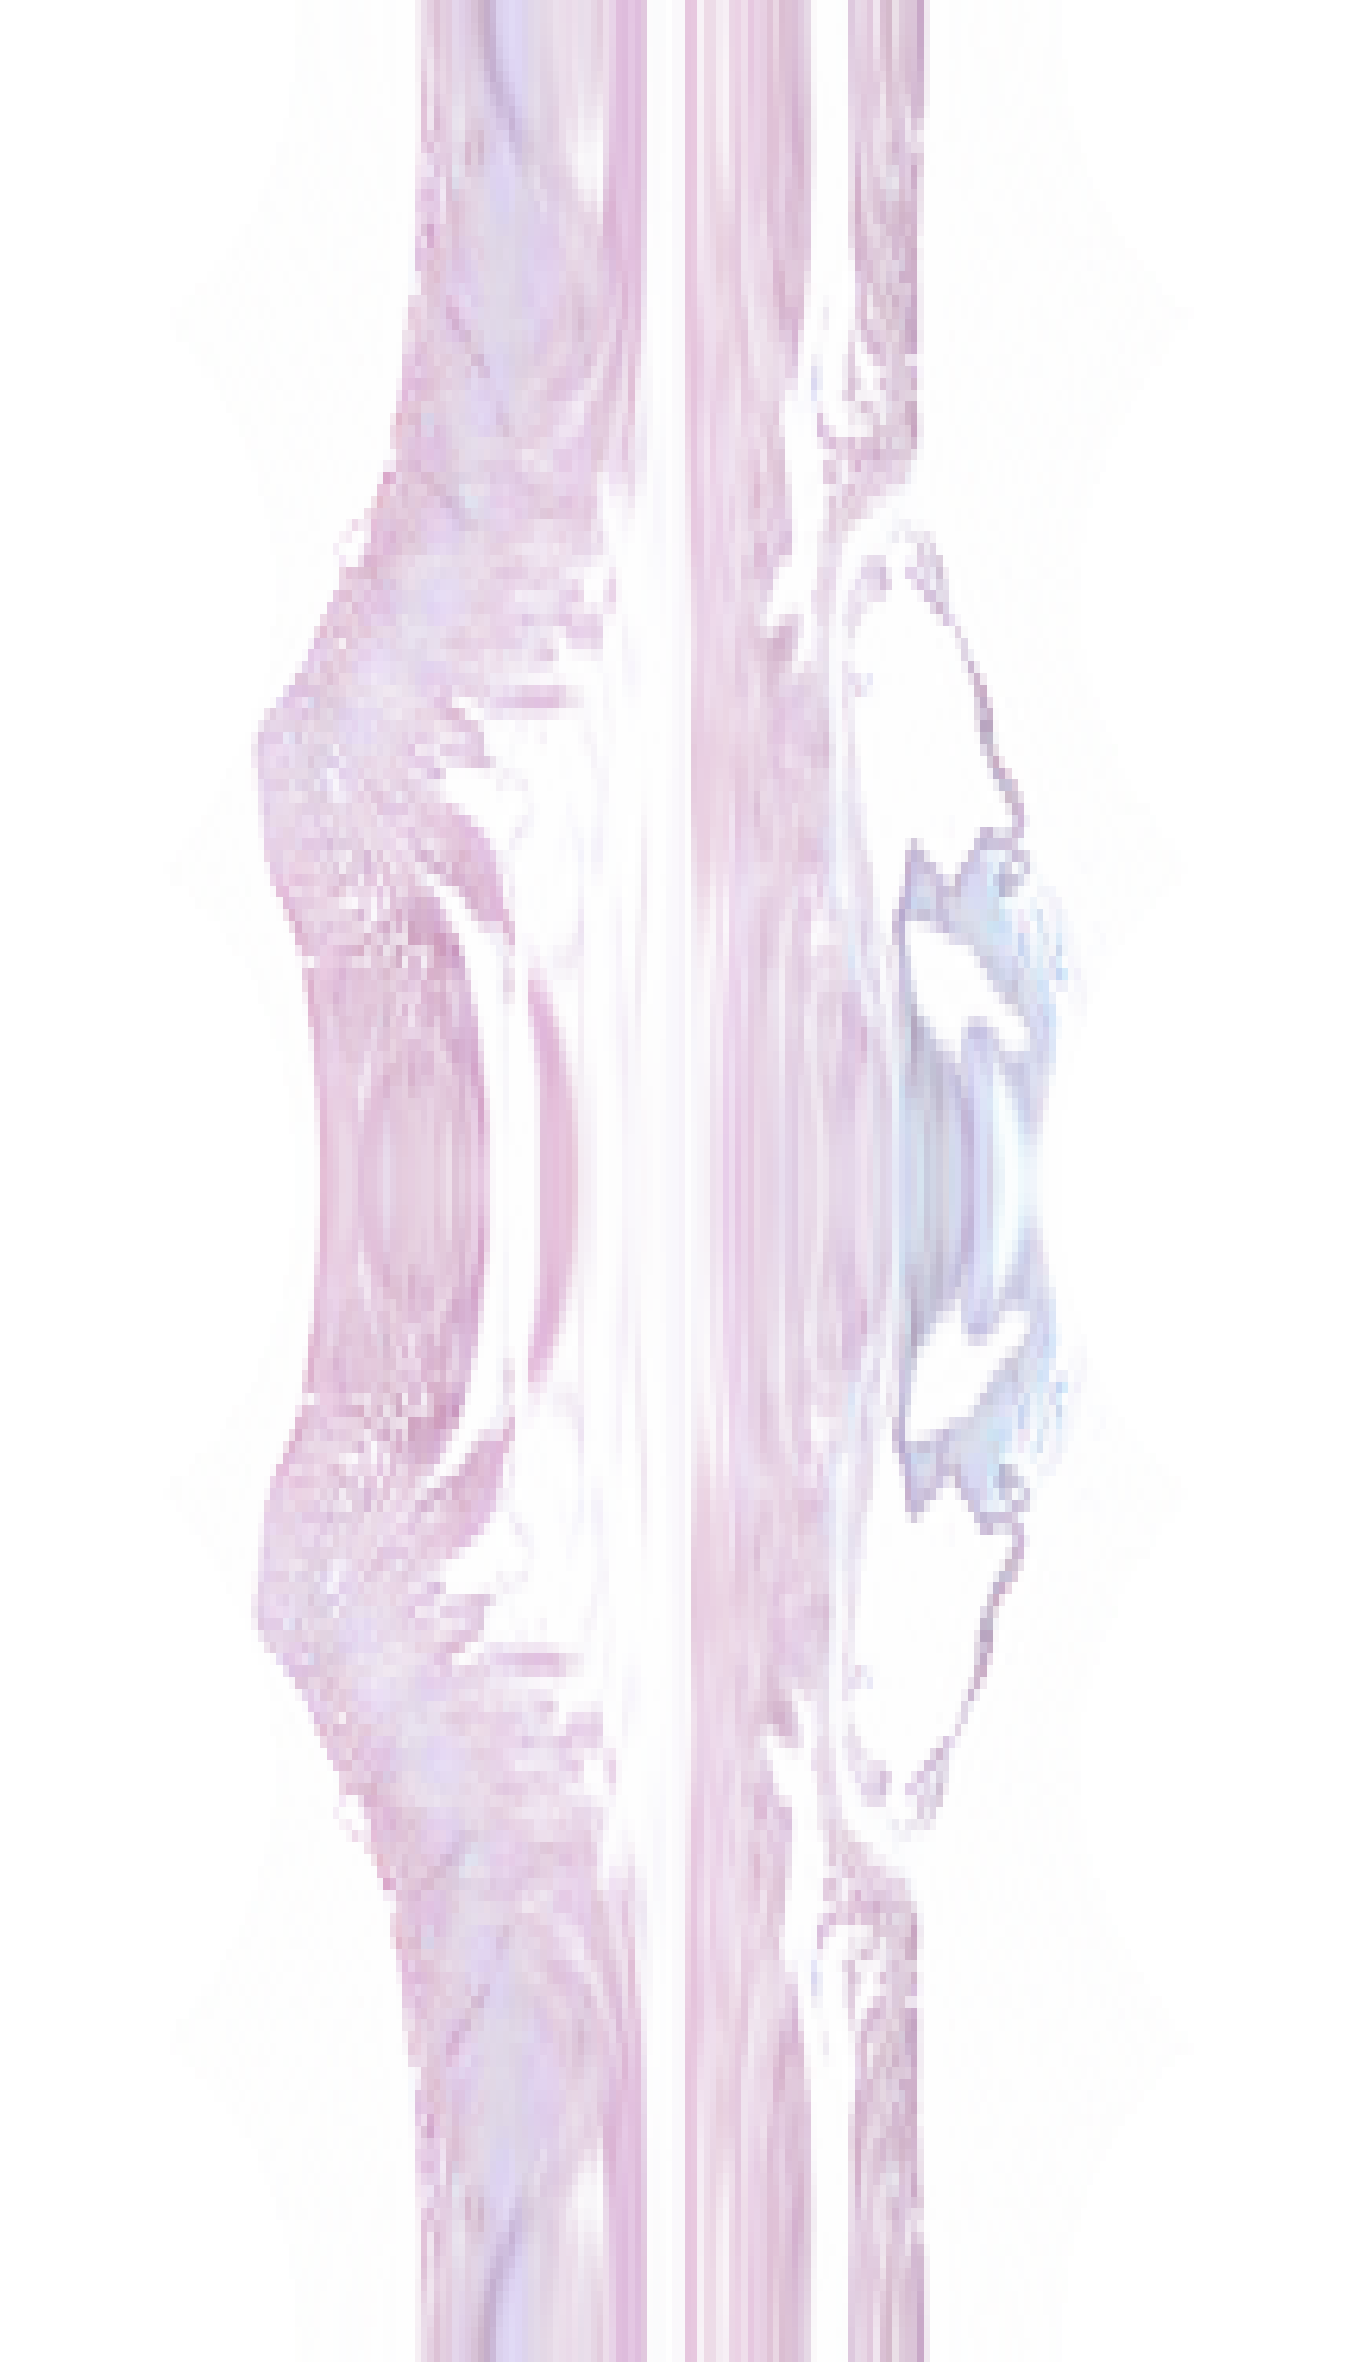
\includegraphics[height=0.33\textheight,type=pdf,ext=.pdf,read=.pdf]{Ch7/Figs/dummies/cross_section_perfect_200_alpha0.4r_0_088}}
    \caption{What a nice figure!}
    \label{fig:dummy_cross_sections}
  \end{sidewaysfigure}
  
  \begin{sidewaysfigure}[htbp]
    \centering
    \subfigure[][0 iterations]{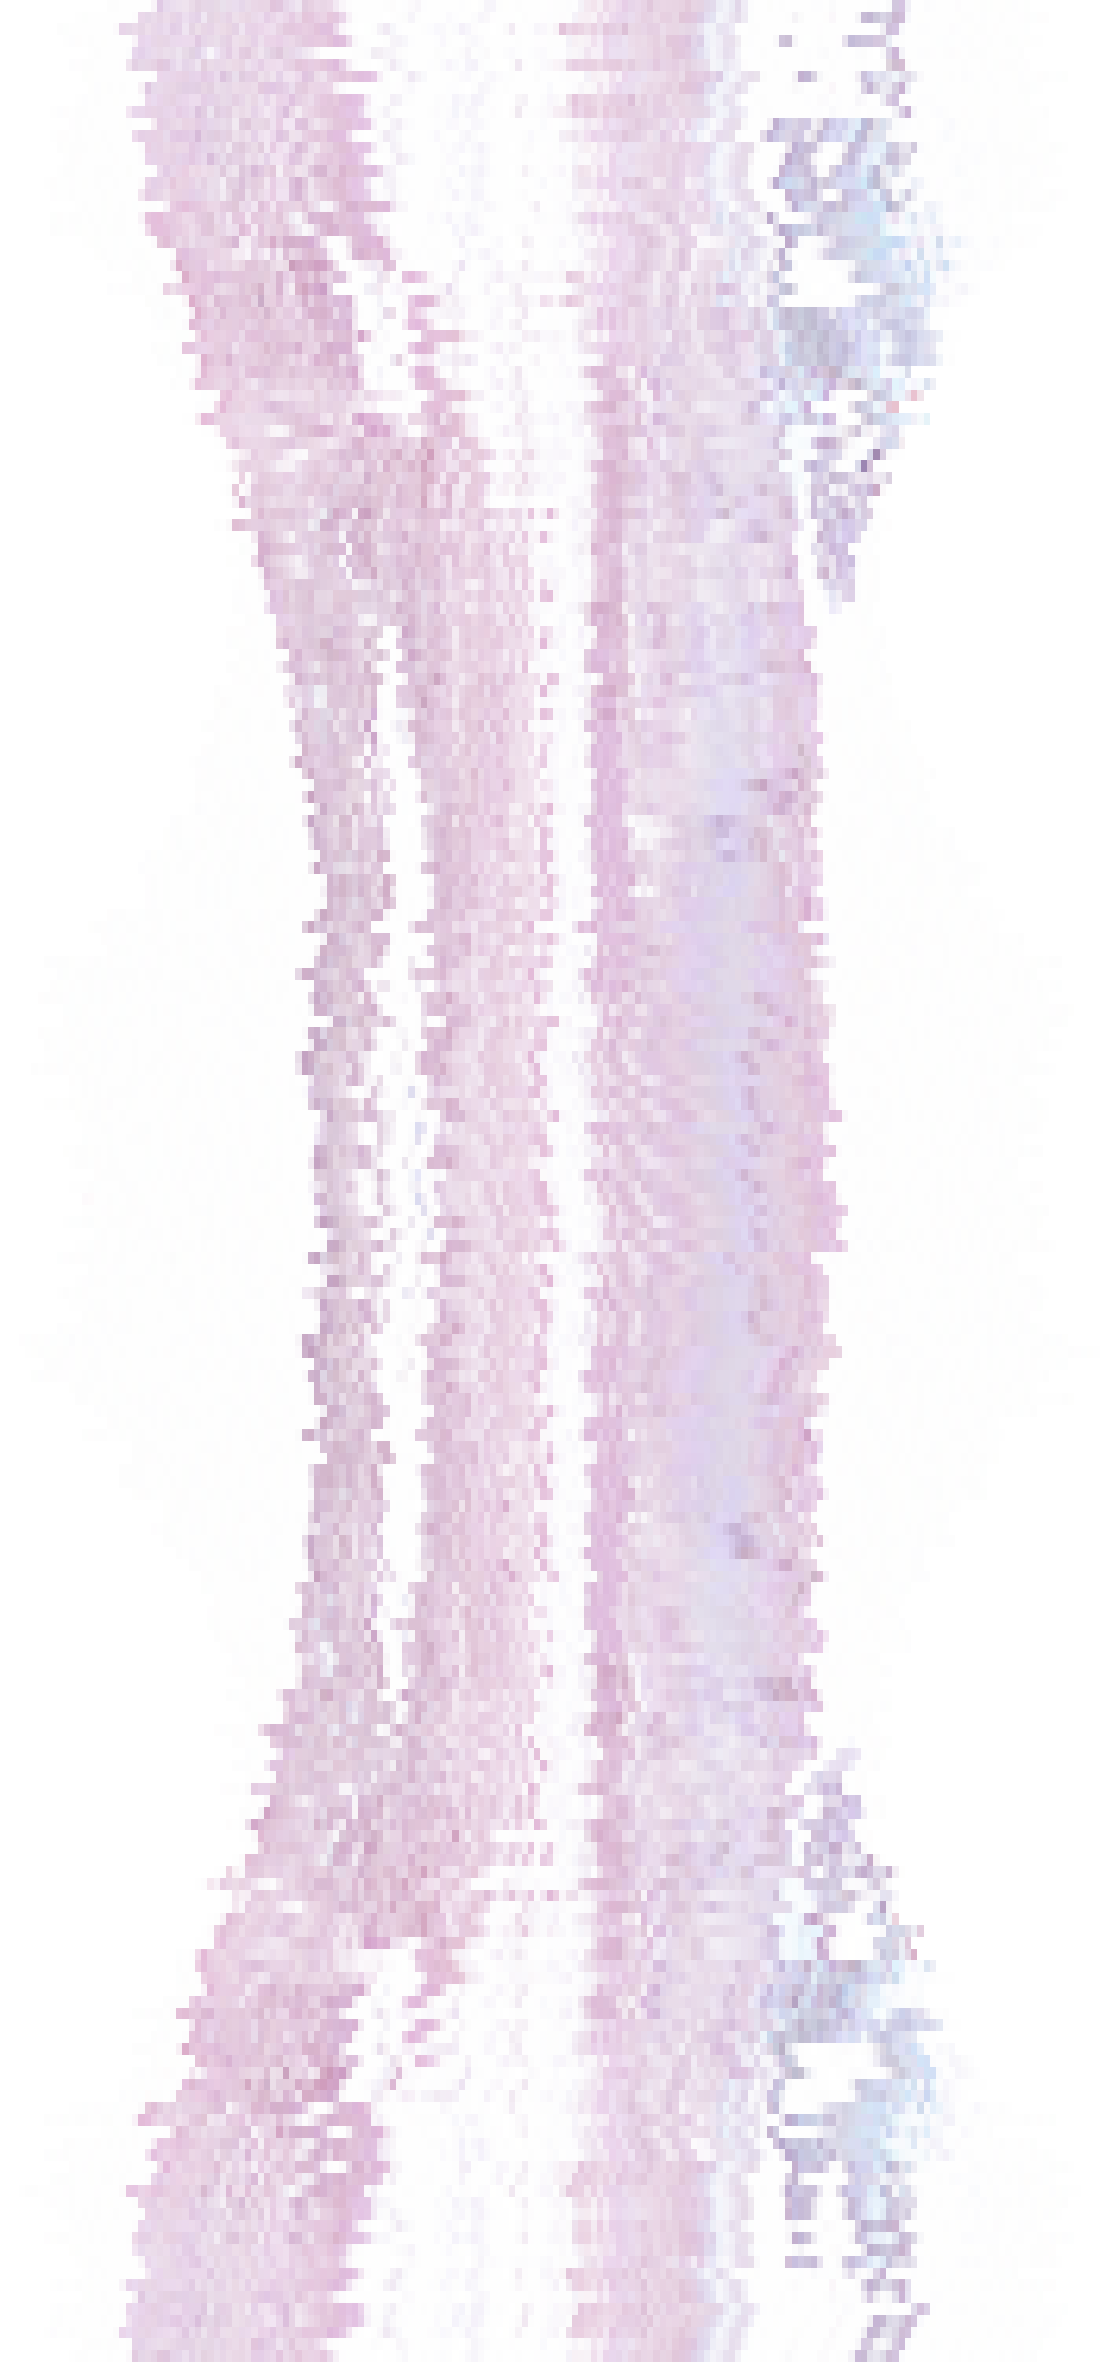
\includegraphics[height=0.33\textheight,type=pdf,ext=.pdf,read=.pdf]{Ch7/Figs/dummies/cross_section_200_alpha0.4r_0_1_107}}
    \subfigure[][1 iteration]{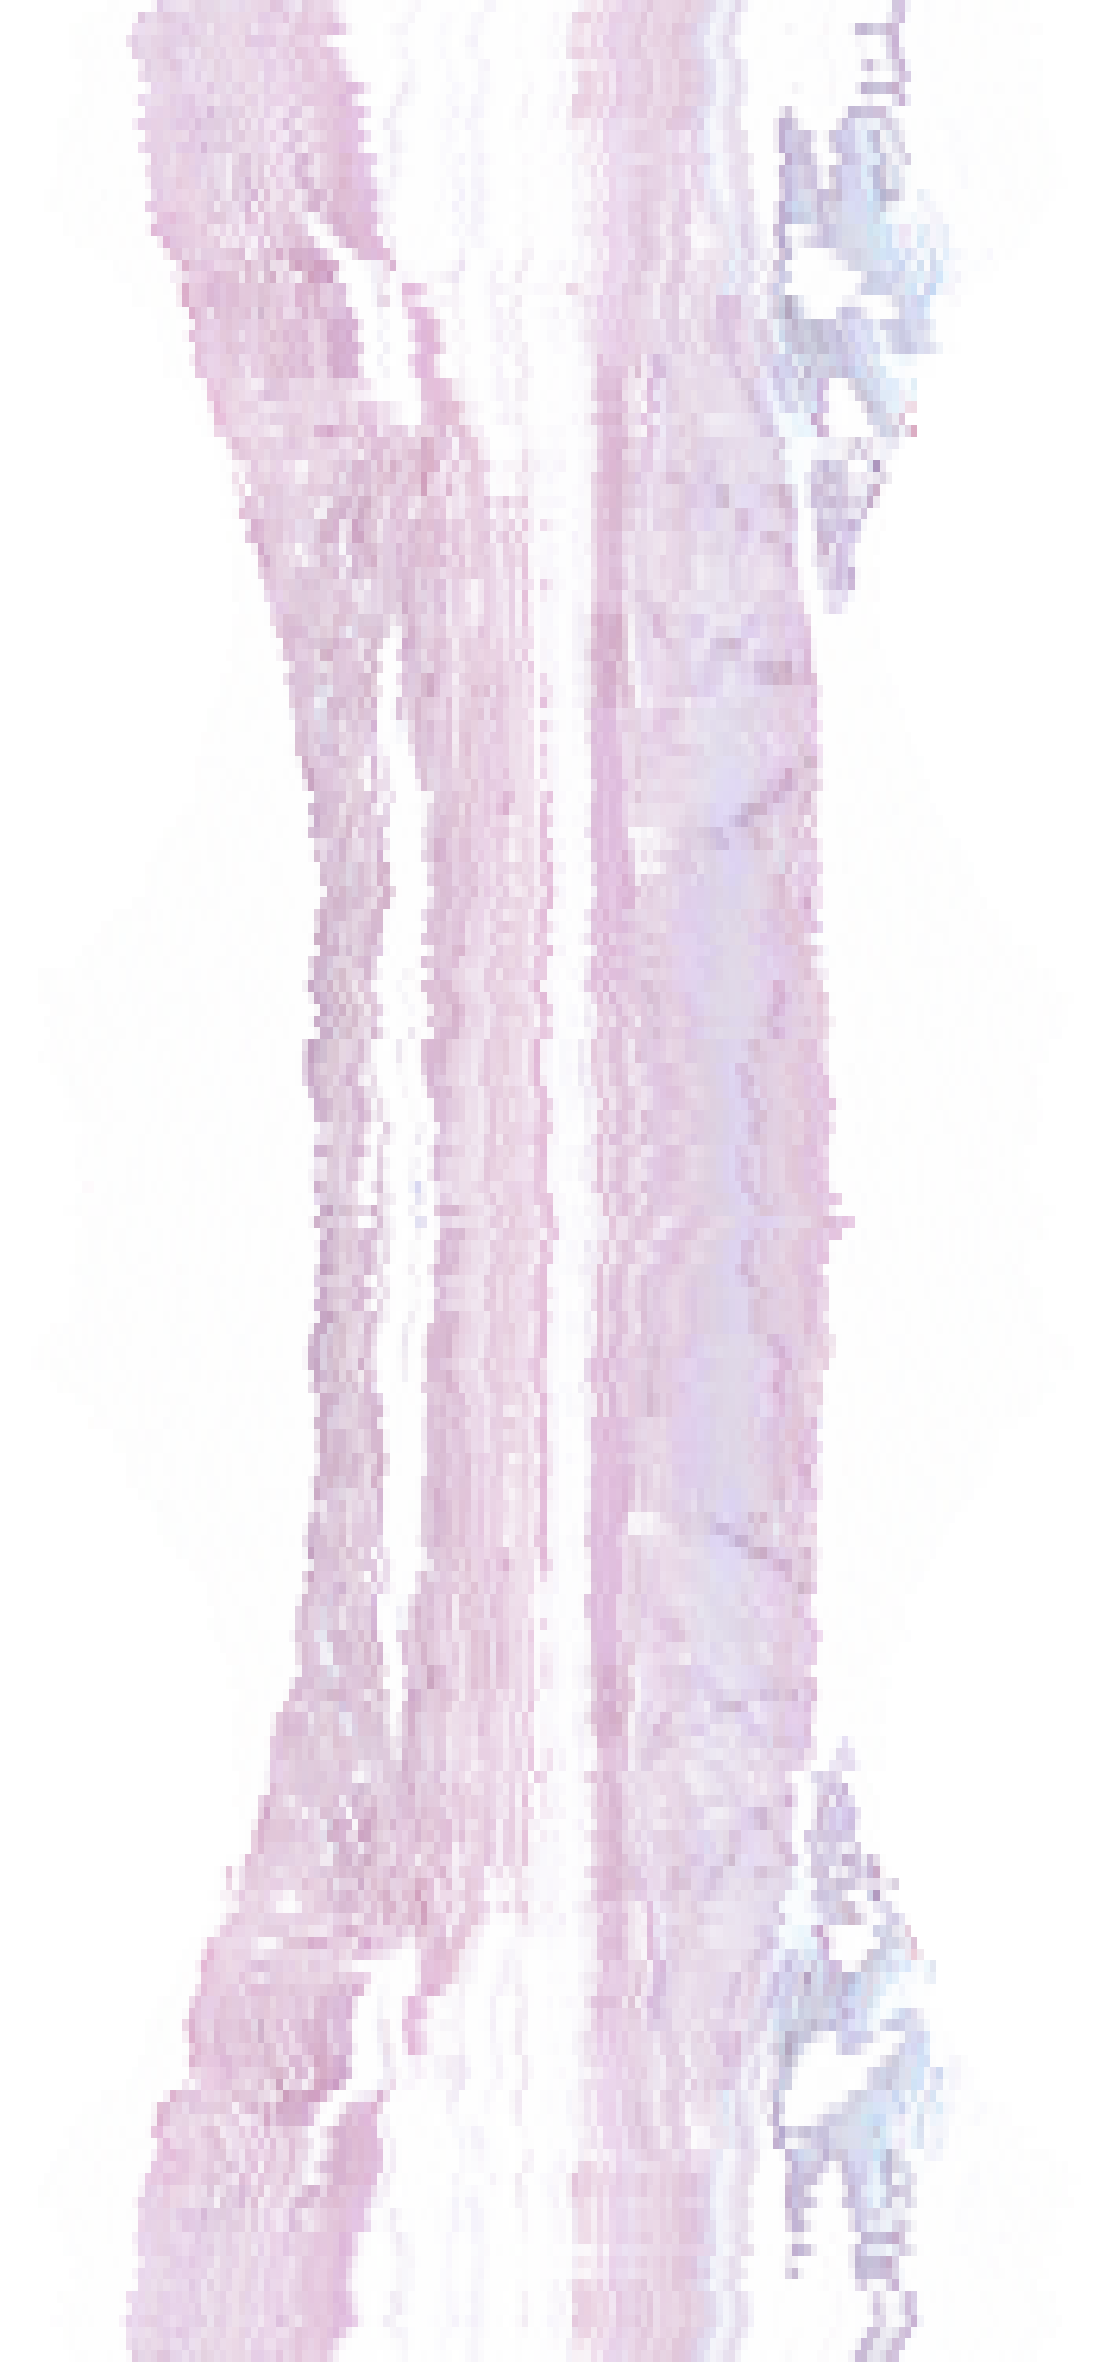
\includegraphics[height=0.33\textheight,type=pdf,ext=.pdf,read=.pdf]{Ch7/Figs/dummies/cross_section_200_alpha0.4r_1_1_107}}
    \subfigure[][3 iterations]{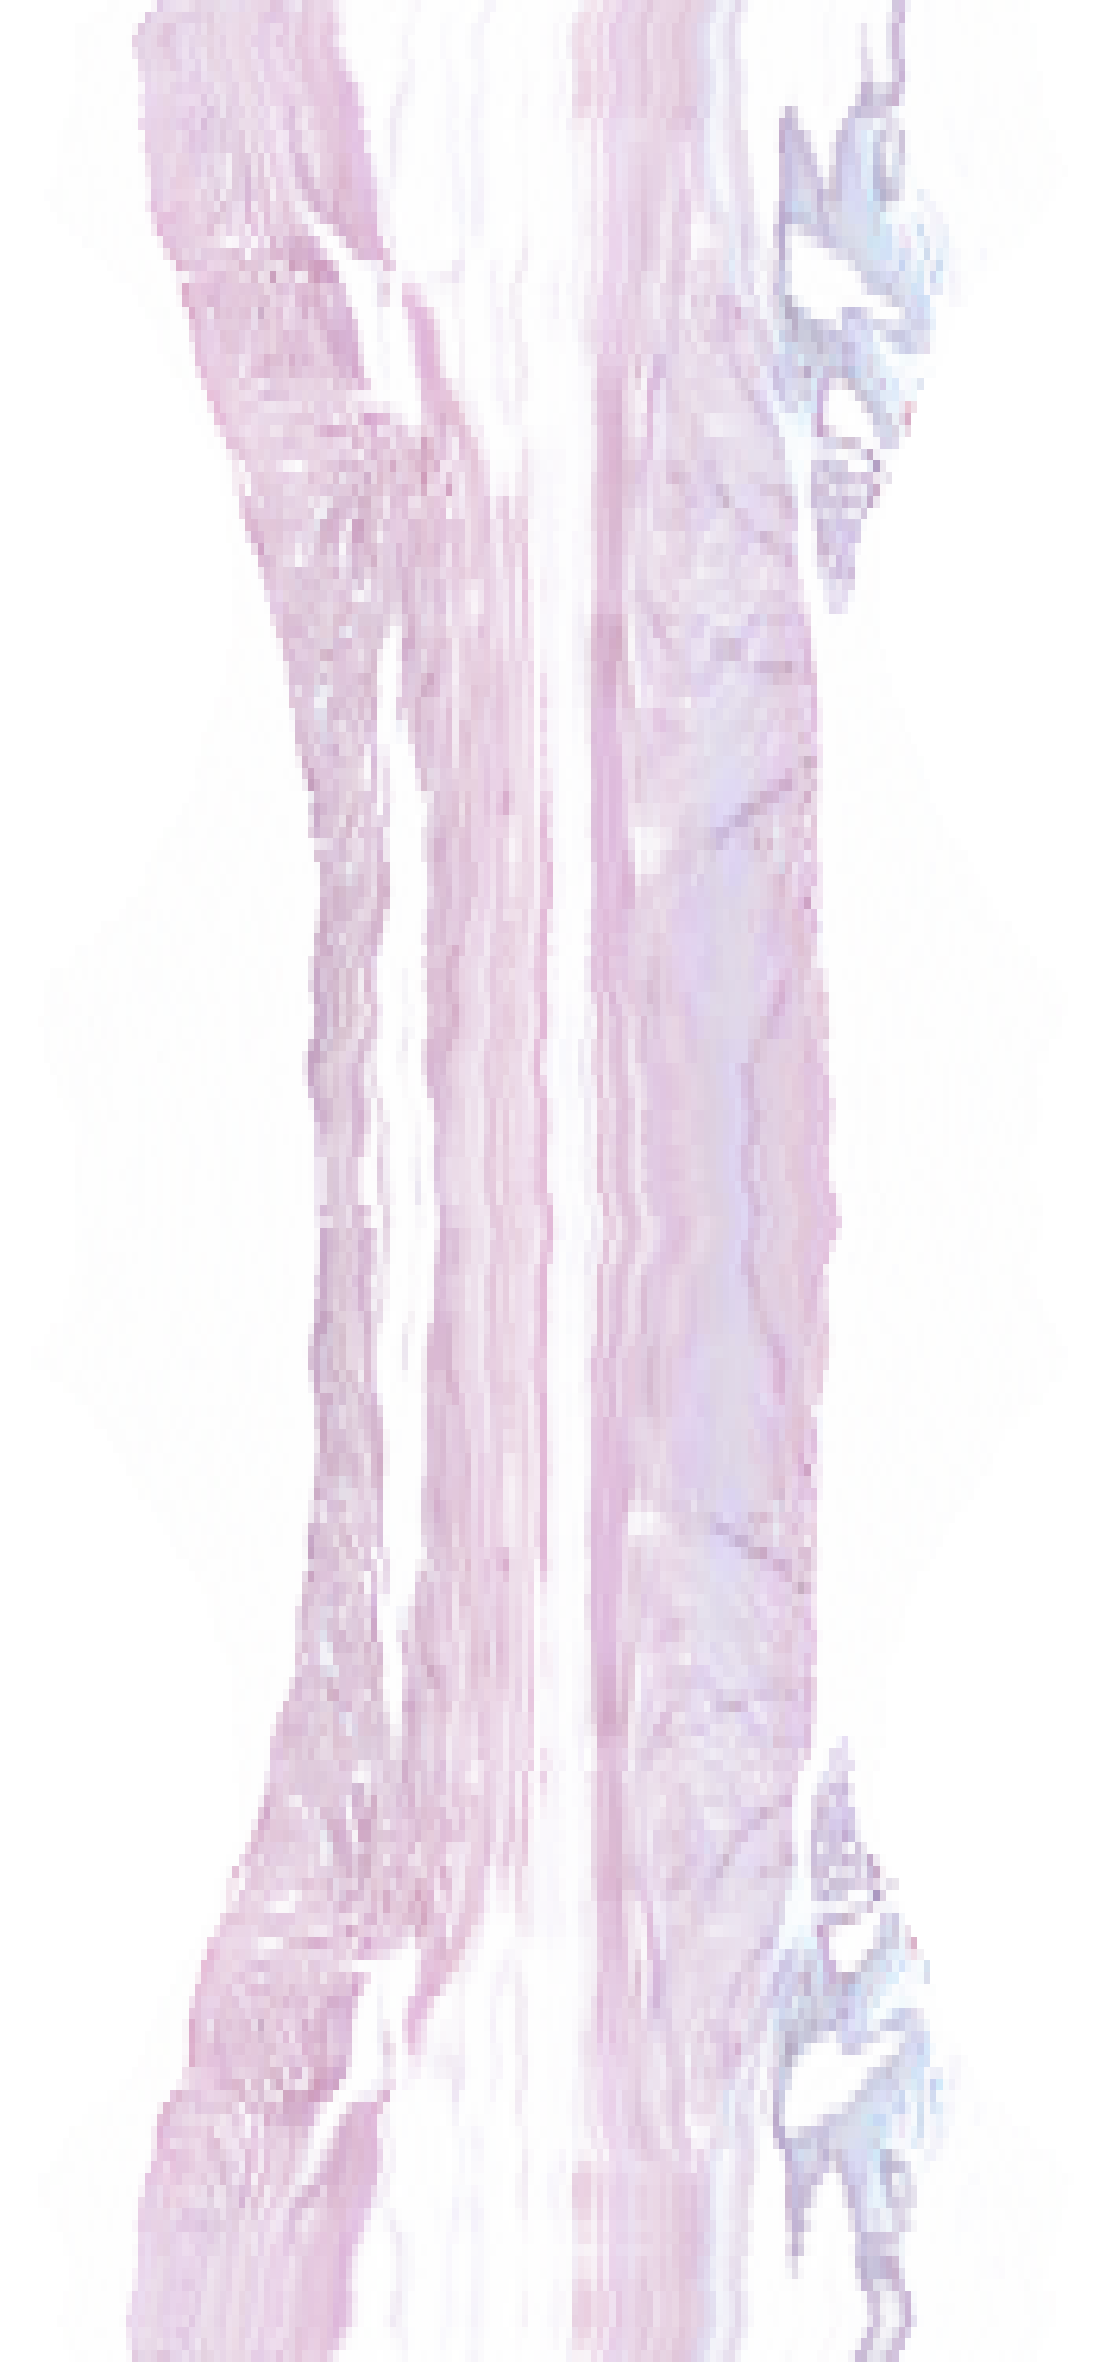
\includegraphics[height=0.33\textheight,type=pdf,ext=.pdf,read=.pdf]{Ch7/Figs/dummies/cross_section_200_alpha0.4r_3_1_107}}
    \subfigure[][10 iterations]{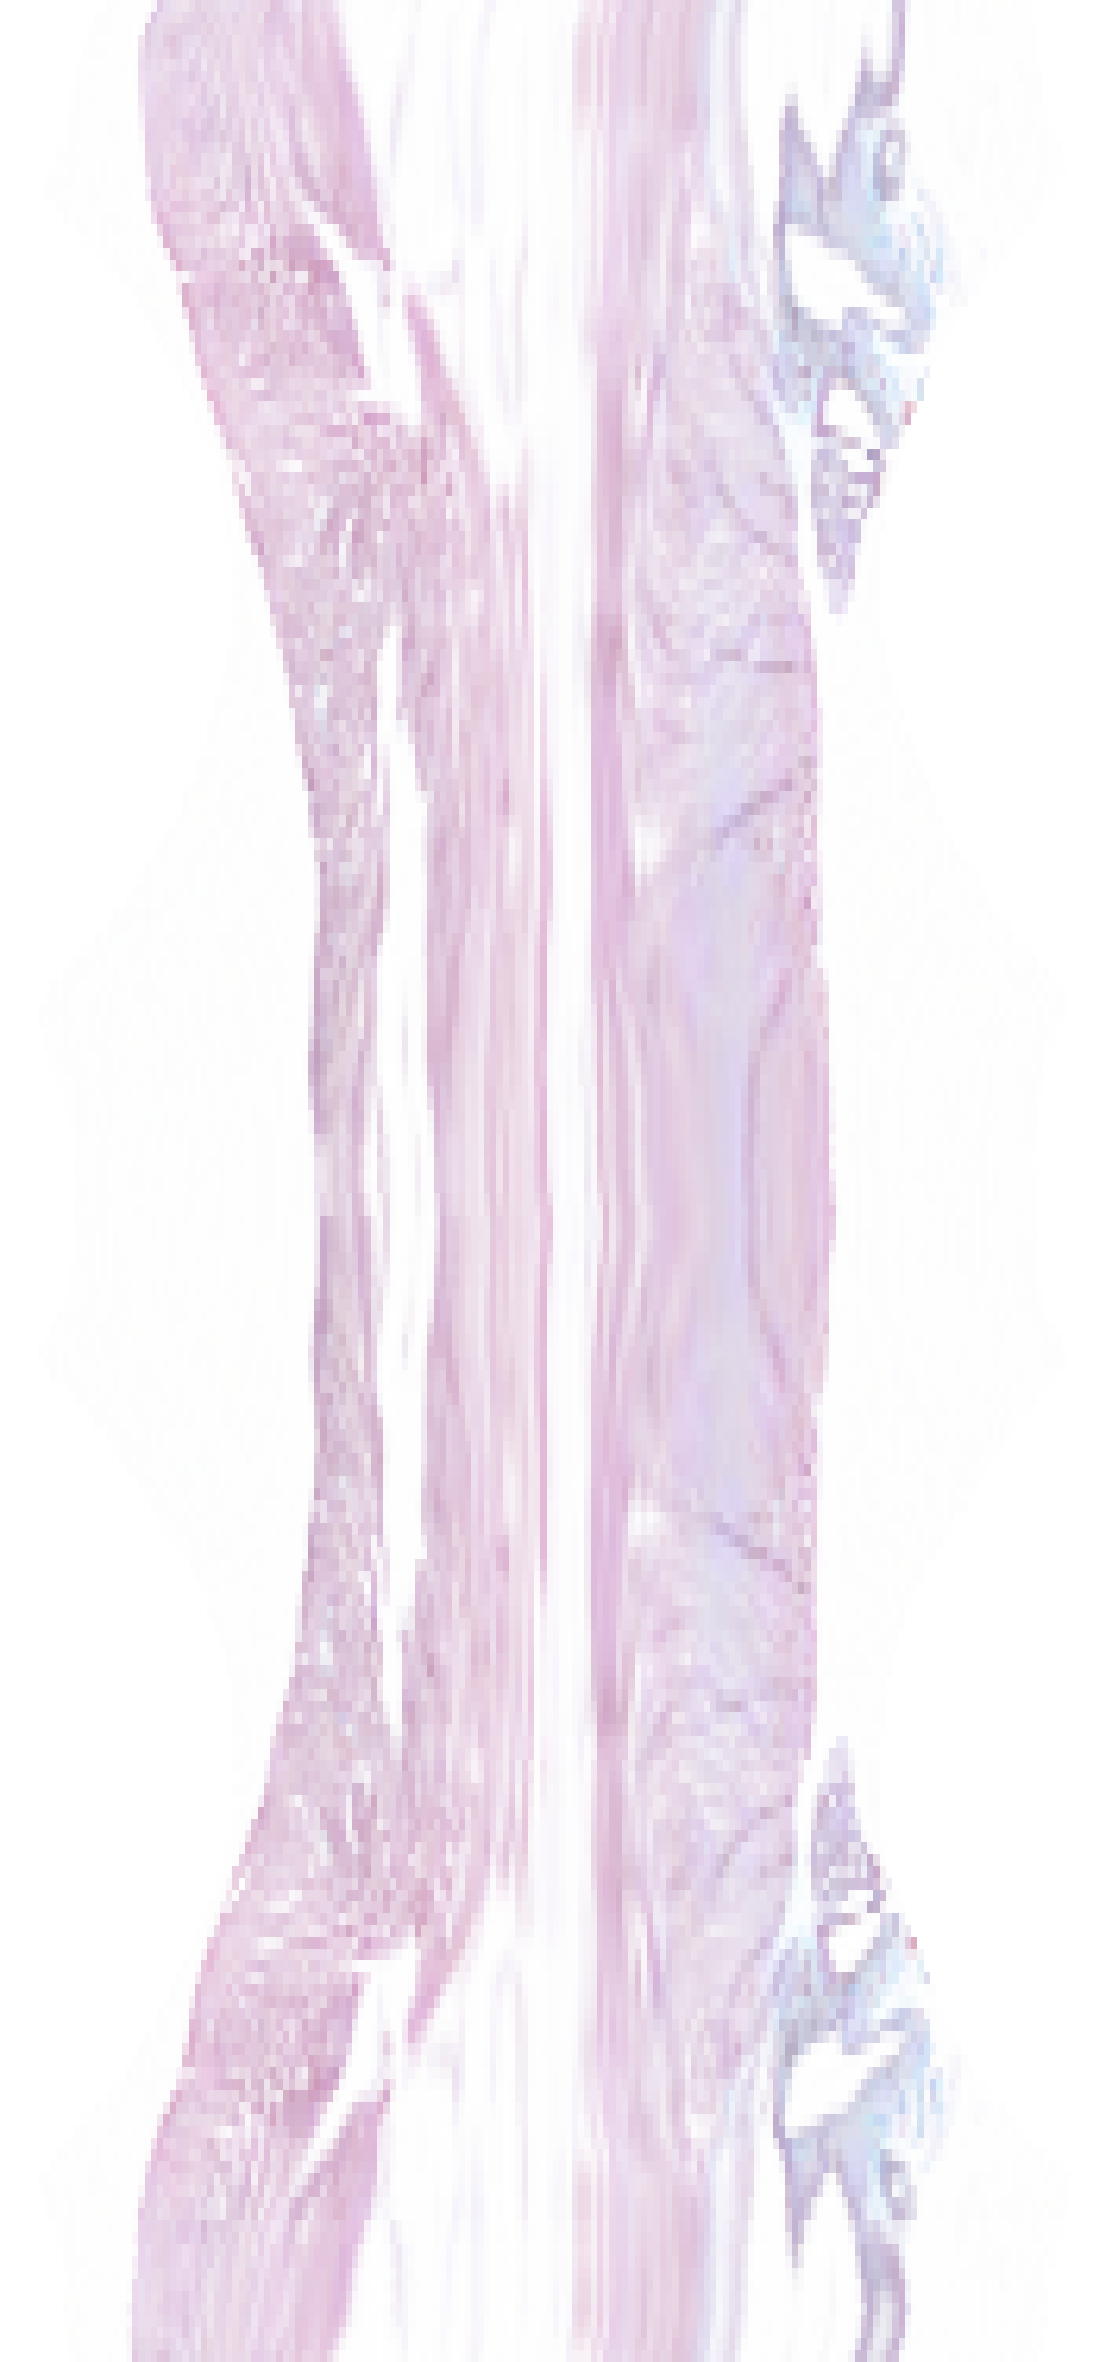
\includegraphics[height=0.33\textheight,type=pdf,ext=.pdf,read=.pdf]{Ch7/Figs/dummies/cross_section_200_alpha0.4r_10_1_107}}
    \subfigure[][without noise]{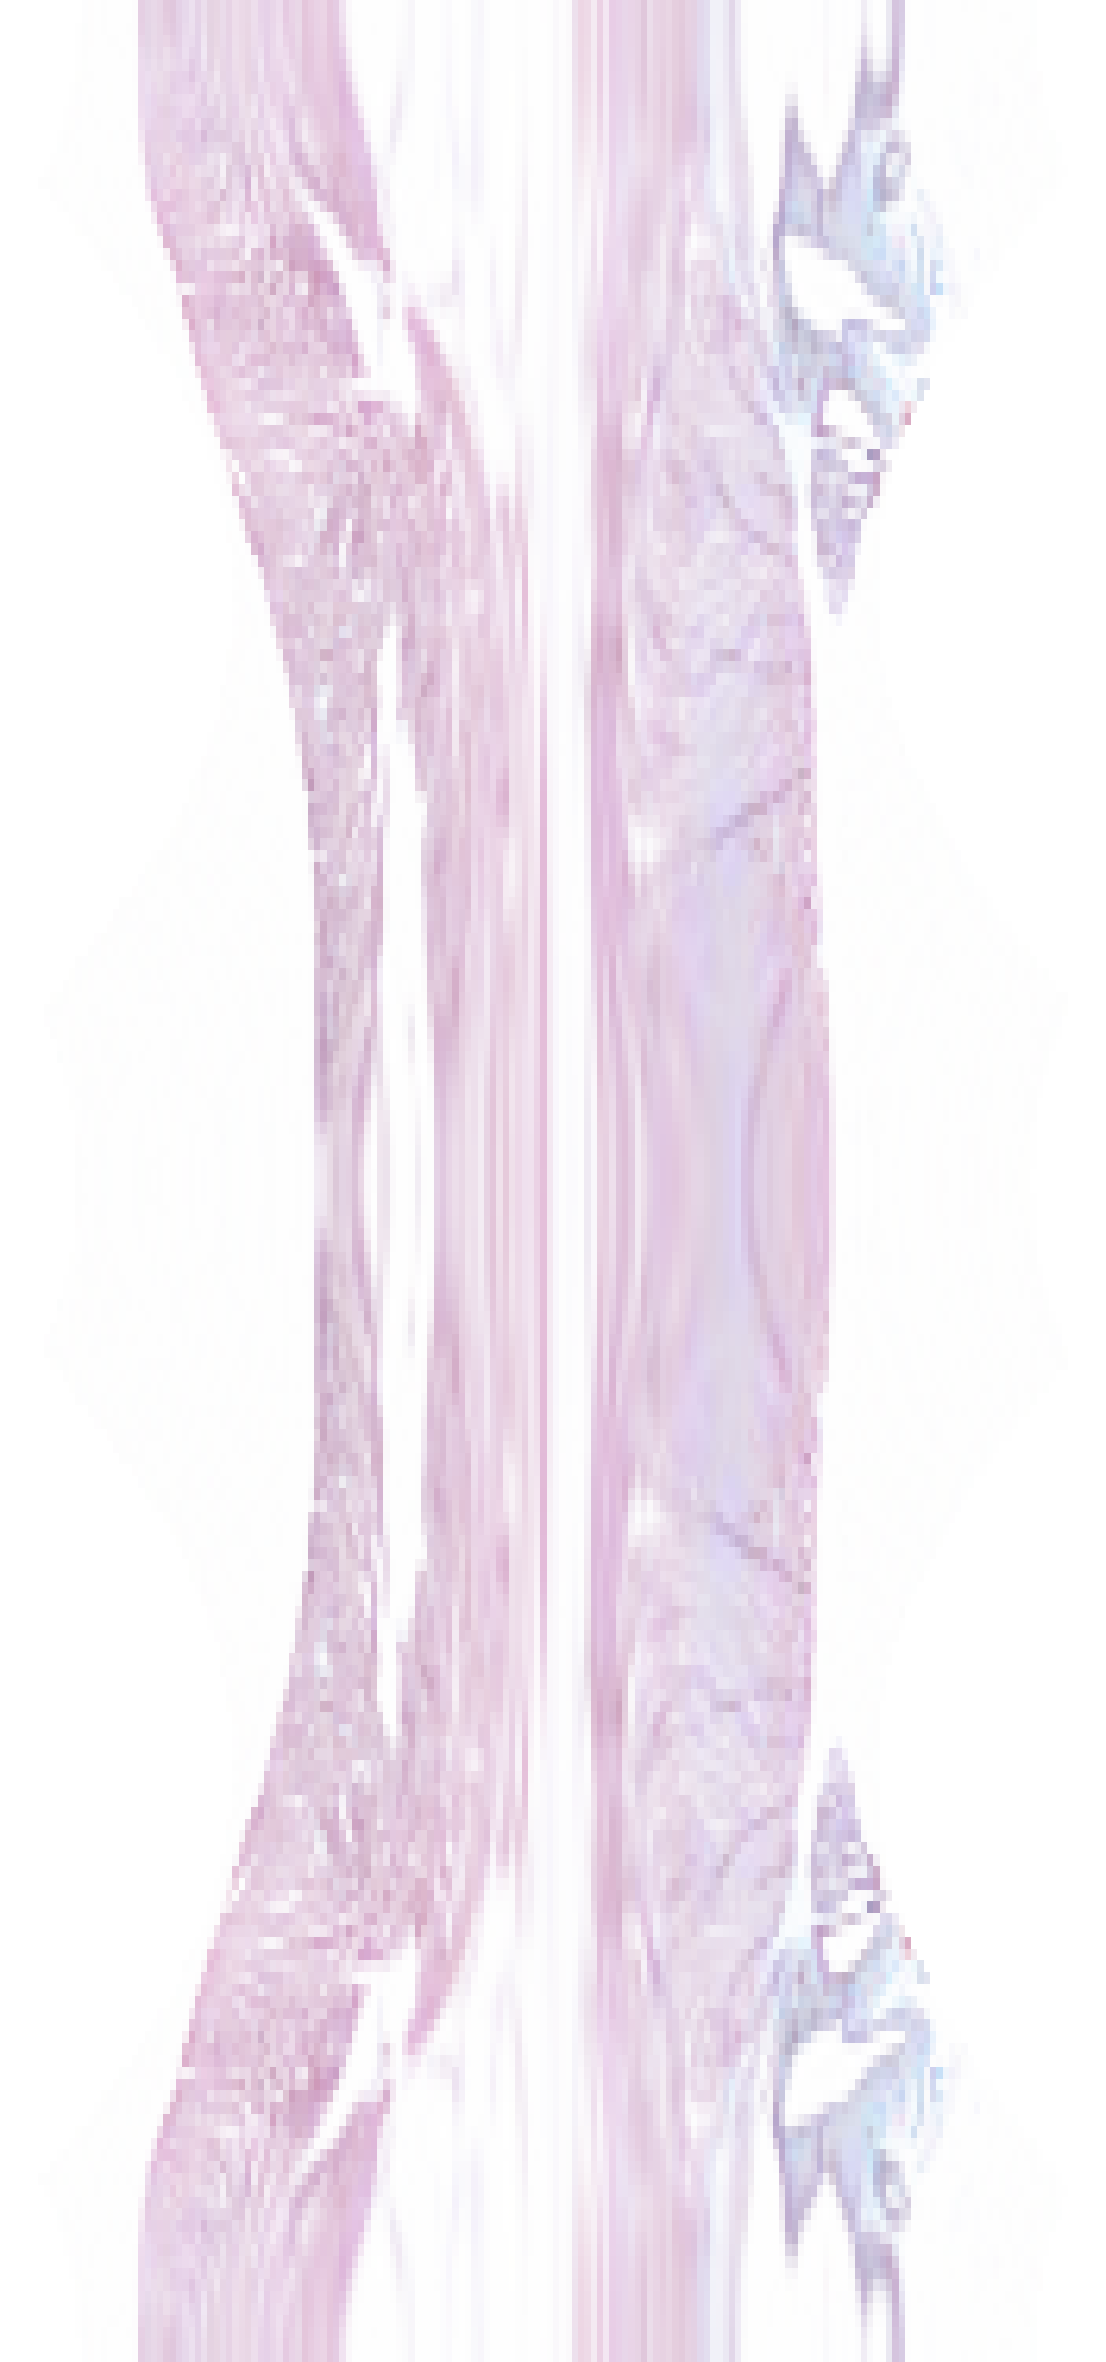
\includegraphics[height=0.33\textheight,type=pdf,ext=.pdf,read=.pdf]{Ch7/Figs/dummies/cross_section_perfect_200_alpha0.4r_1_107}}
    \caption{What a nice figure!}
    \label{fig:dummy_cross_sections}
  \end{sidewaysfigure}
  
  % translated
  \begin{sidewaysfigure}[htbp]
    \centering
    \subfigure[][0 iterations]{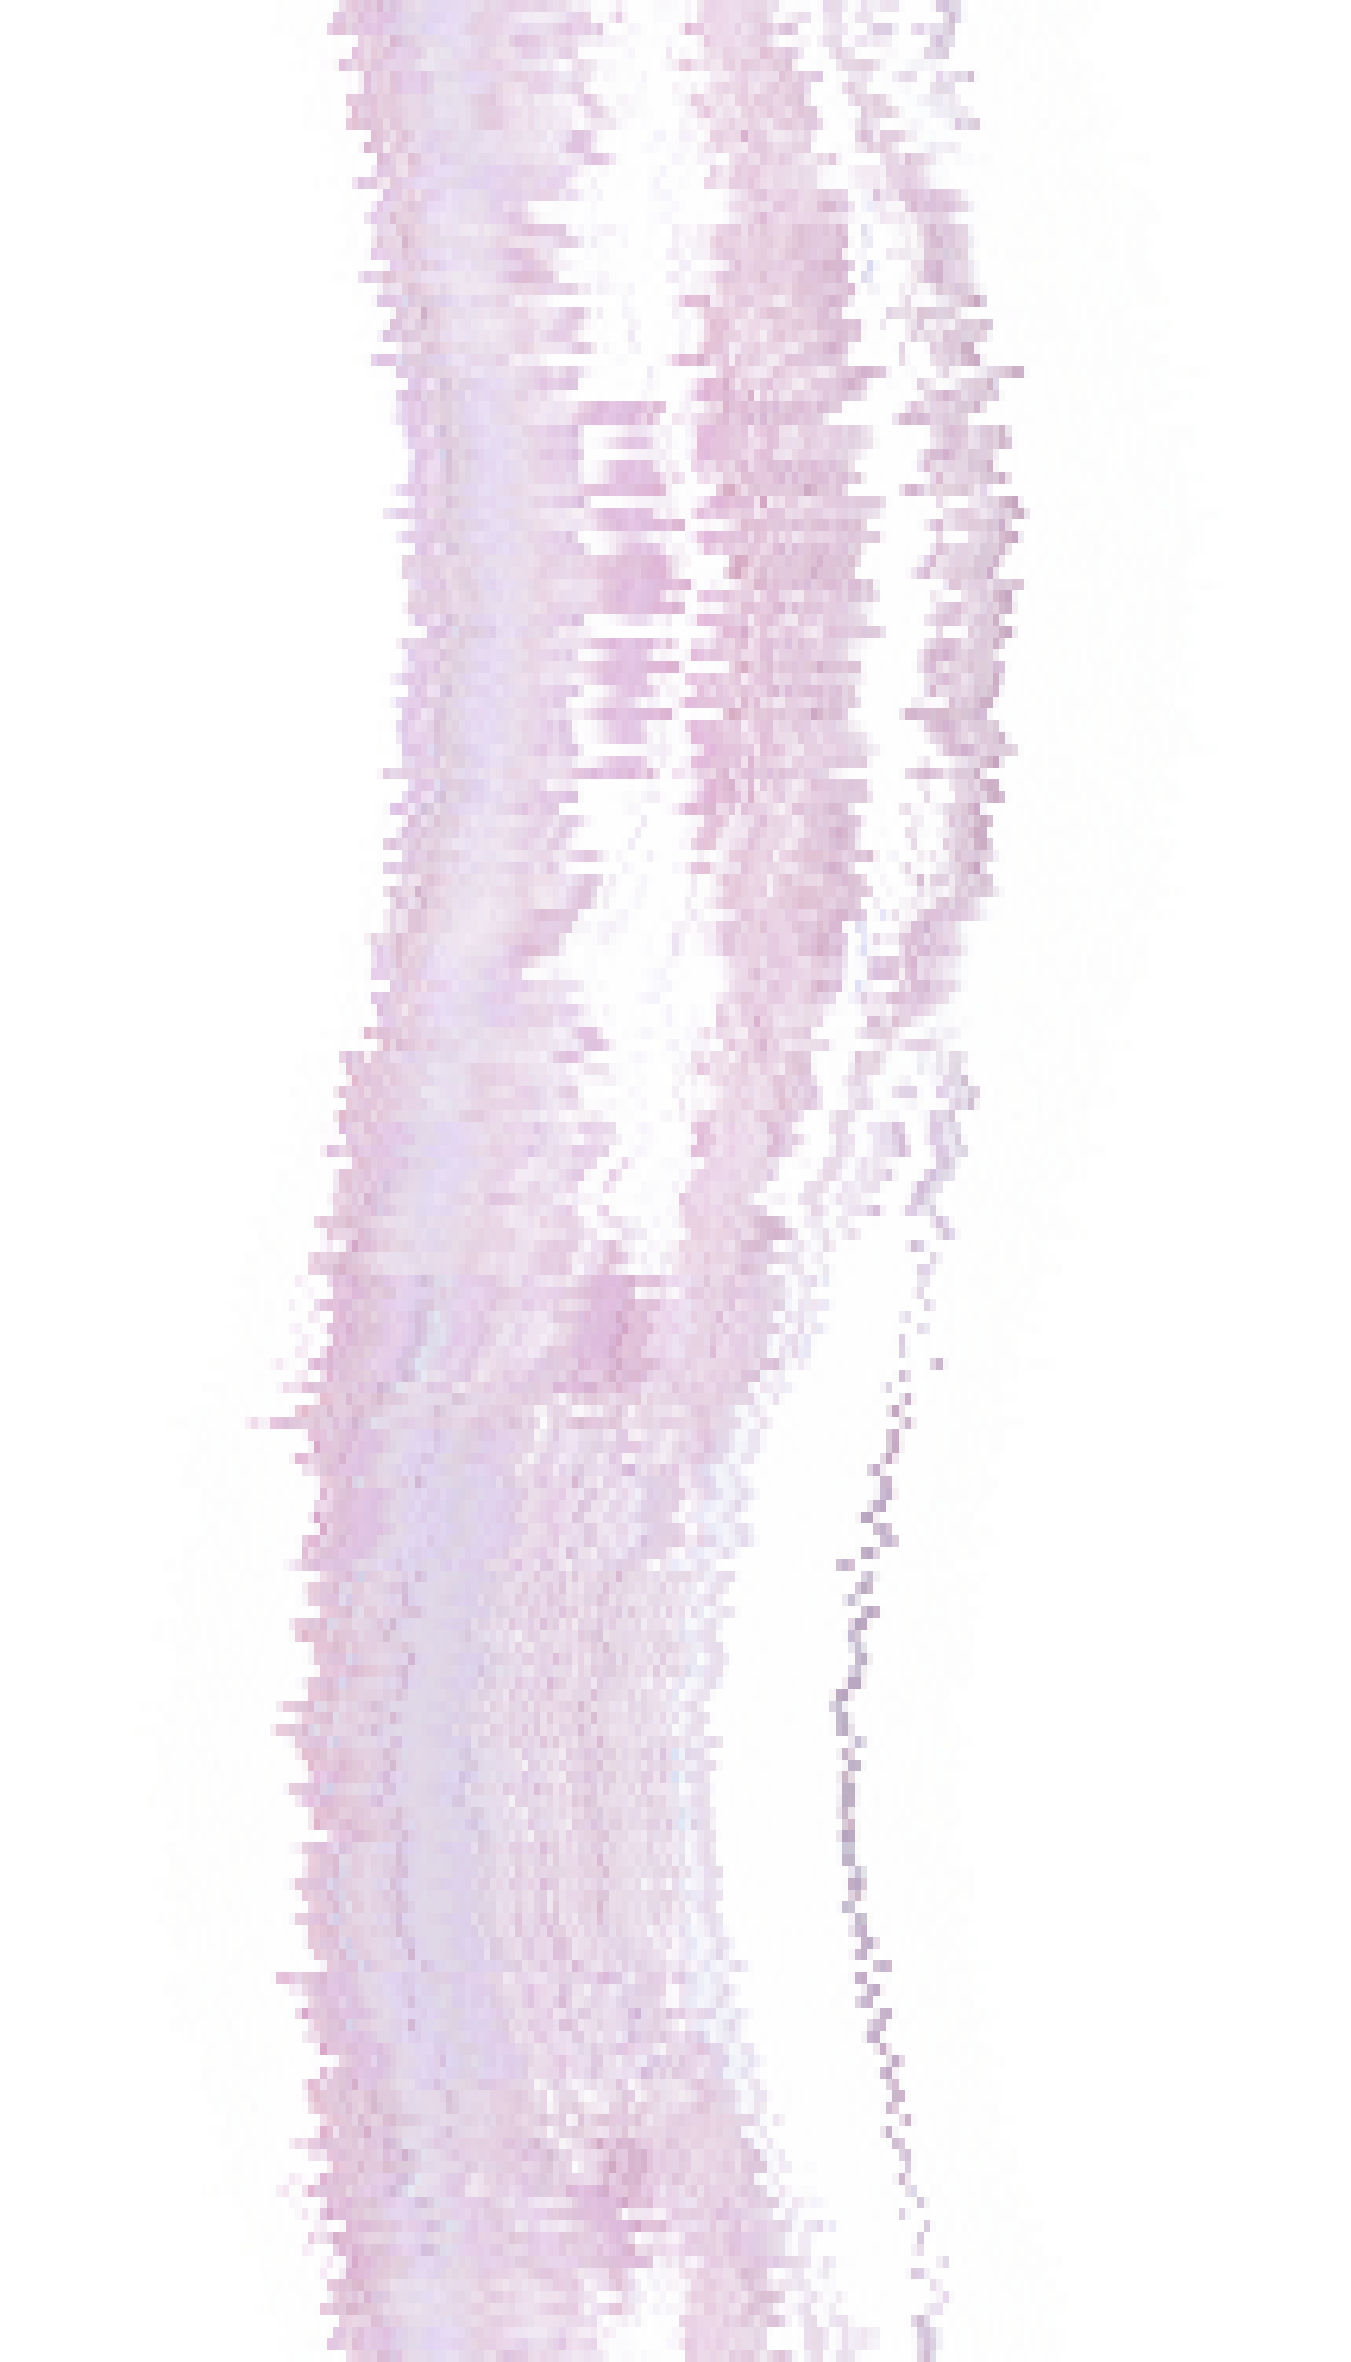
\includegraphics[height=0.33\textheight,type=pdf,ext=.pdf,read=.pdf]{Ch7/Figs/dummies/cross_section_200_alpha0.4t_0_0_088}}
    \subfigure[][1 iteration]{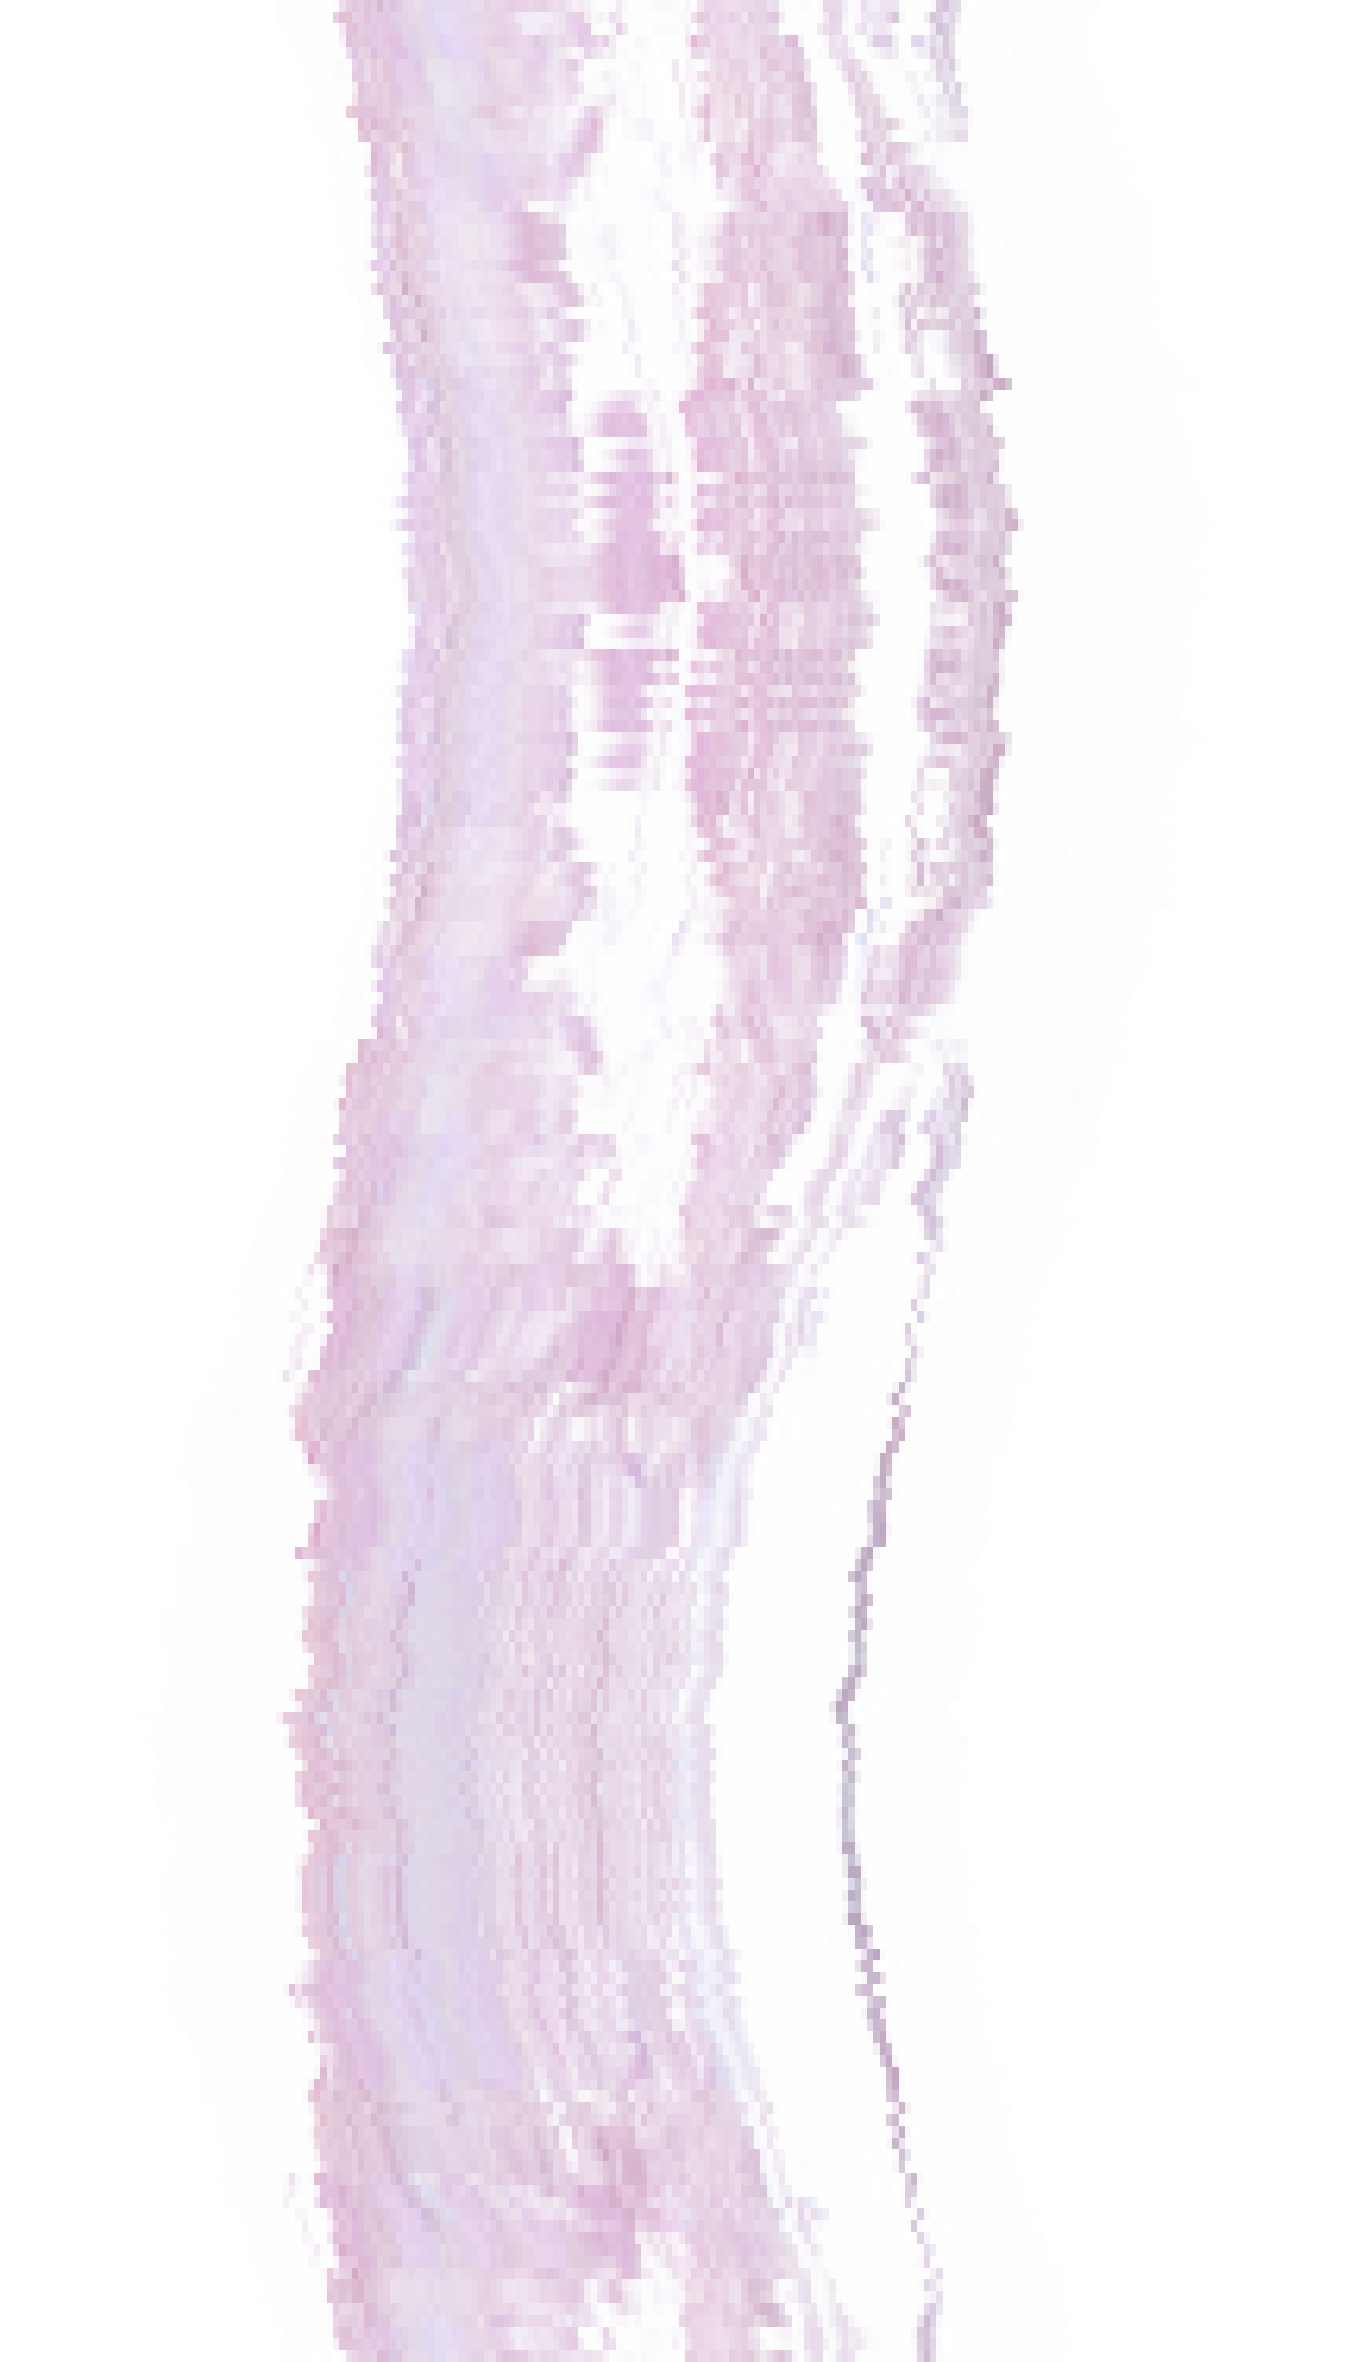
\includegraphics[height=0.33\textheight,type=pdf,ext=.pdf,read=.pdf]{Ch7/Figs/dummies/cross_section_200_alpha0.4t_1_0_088}}
    \subfigure[][3 iterations]{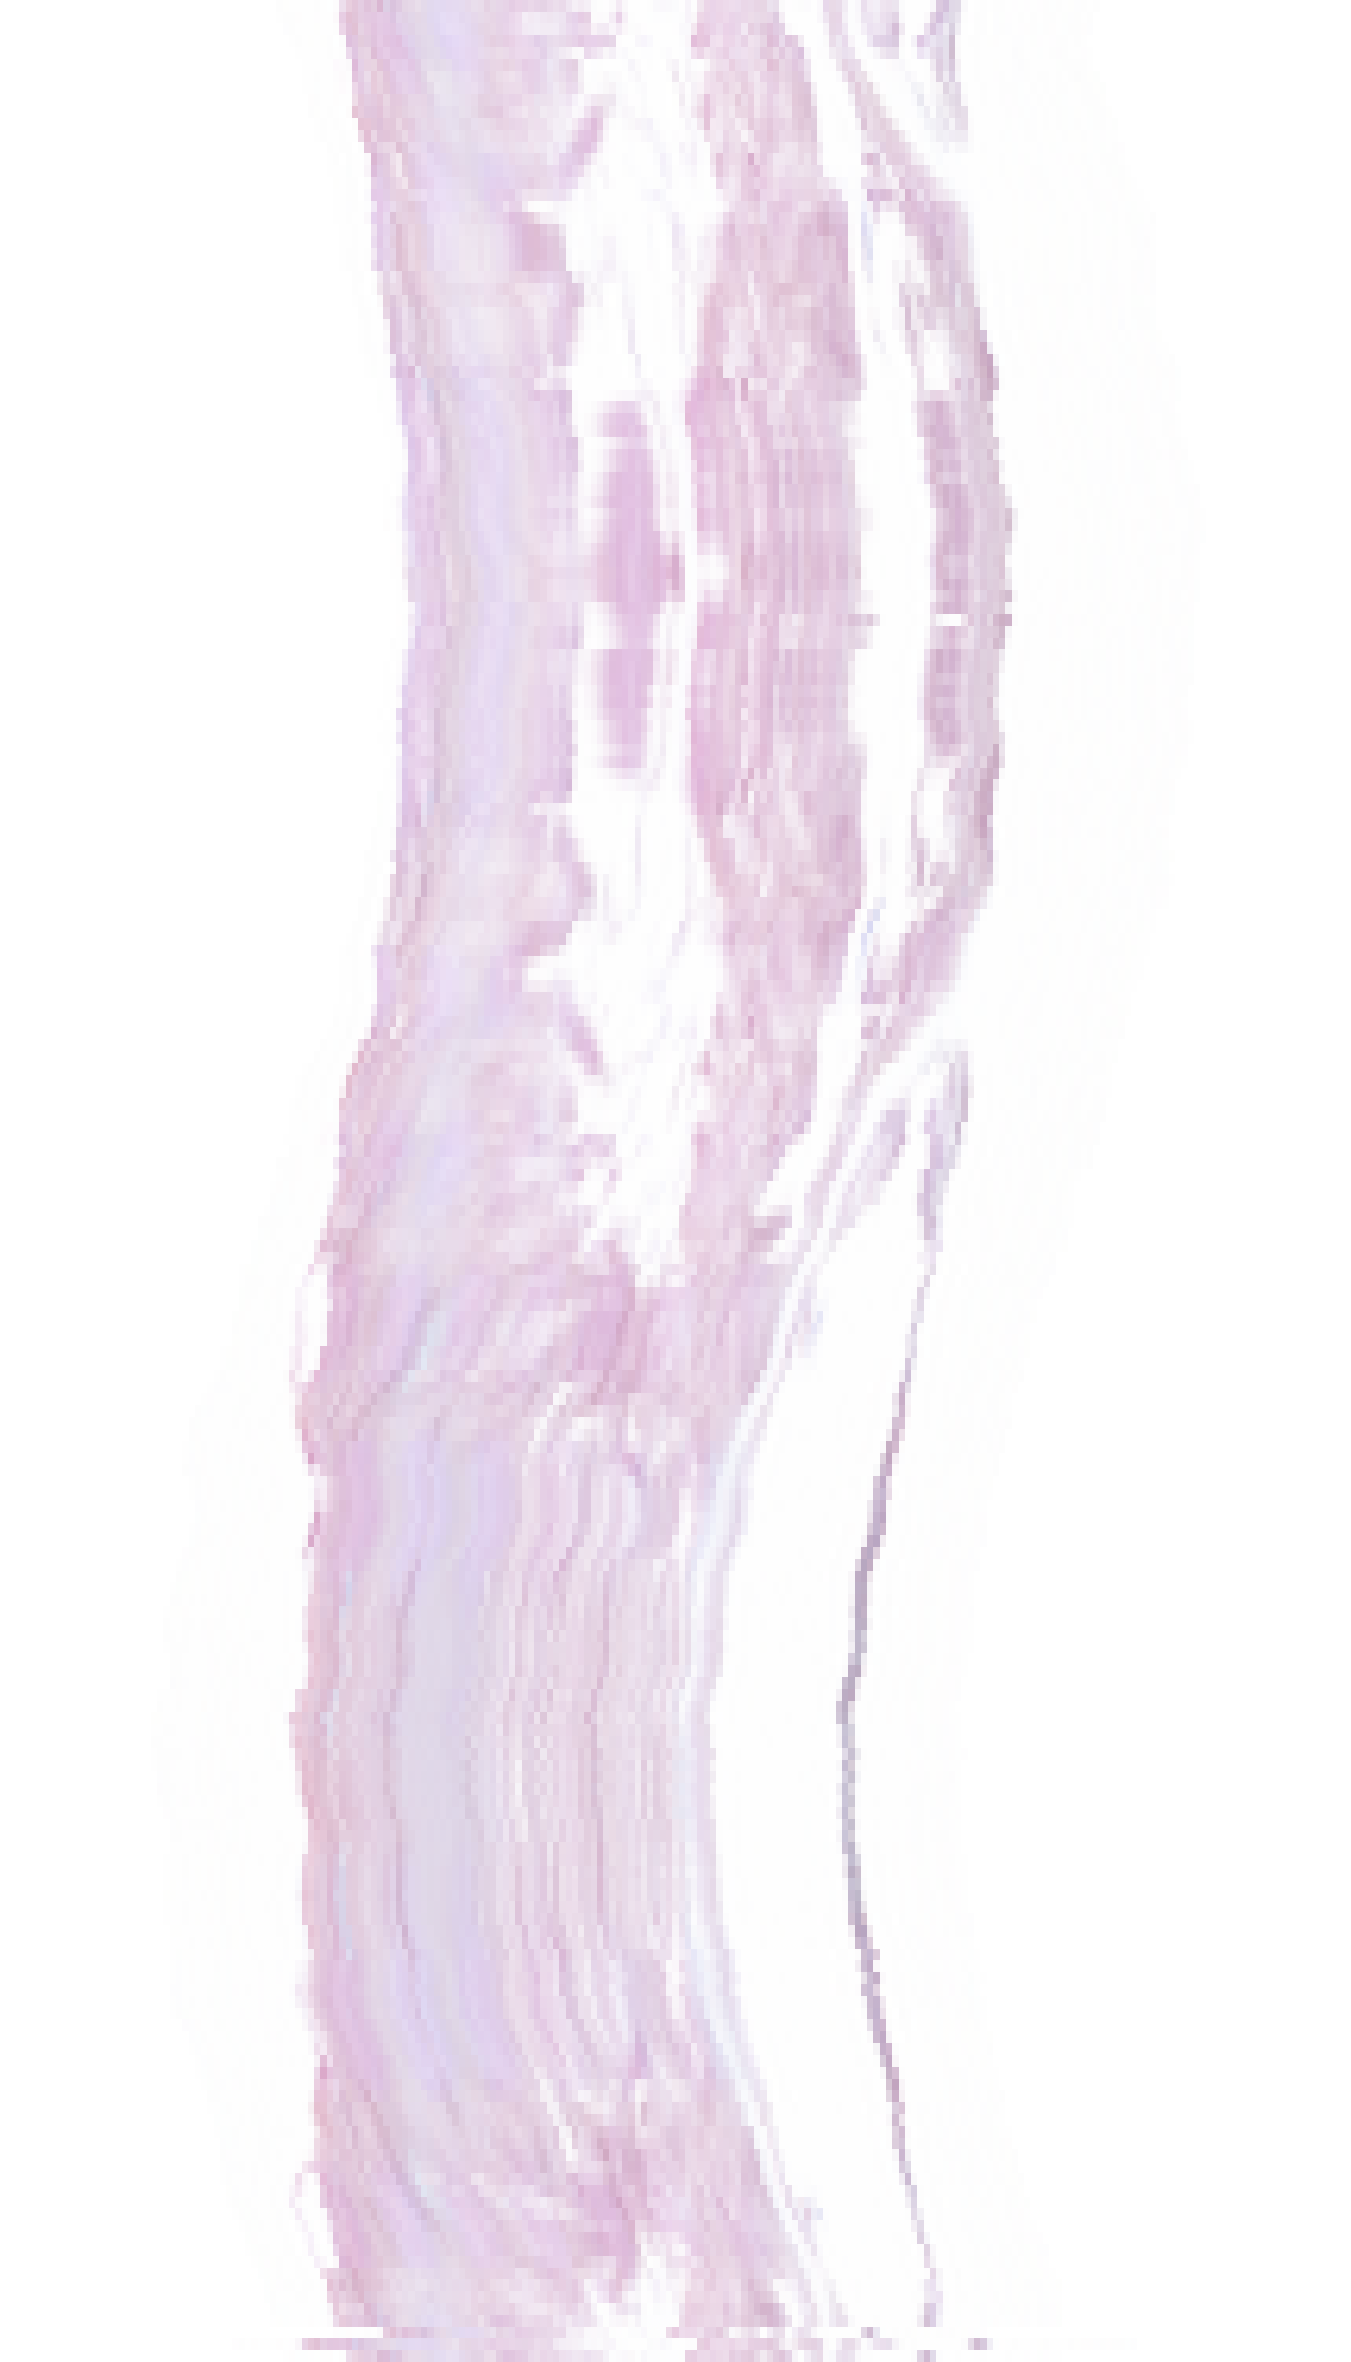
\includegraphics[height=0.33\textheight,type=pdf,ext=.pdf,read=.pdf]{Ch7/Figs/dummies/cross_section_200_alpha0.4t_3_0_088}}
    \subfigure[][10 iterations]{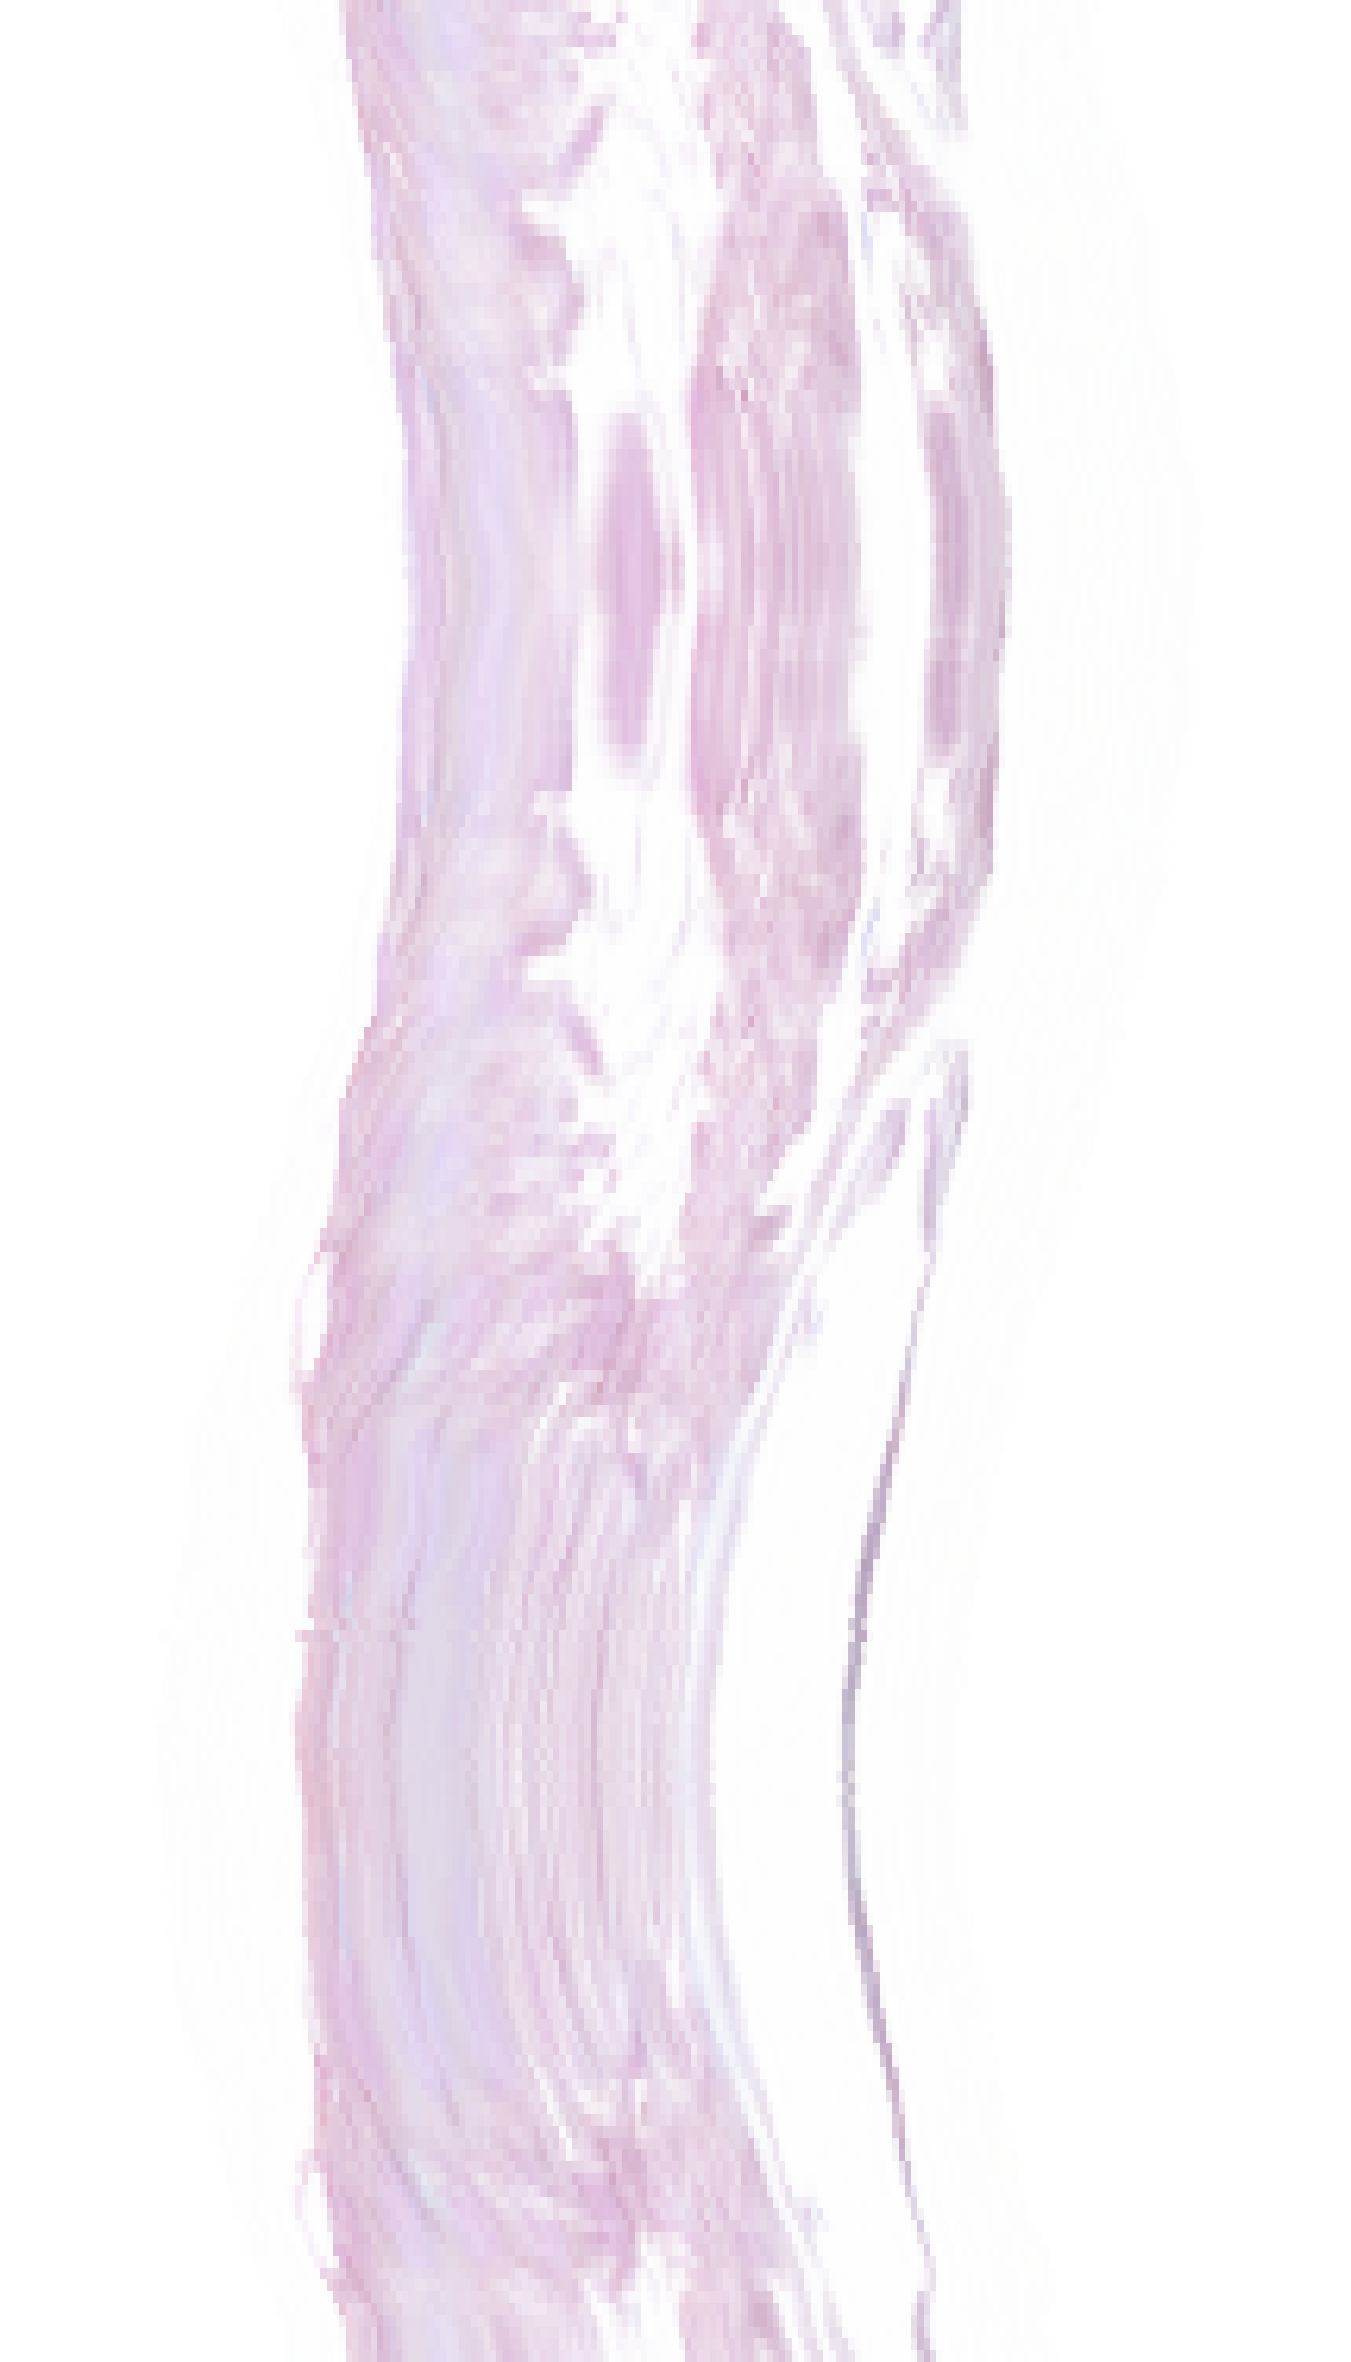
\includegraphics[height=0.33\textheight,type=pdf,ext=.pdf,read=.pdf]{Ch7/Figs/dummies/cross_section_200_alpha0.4t_10_0_088}}
    \subfigure[][without noise]{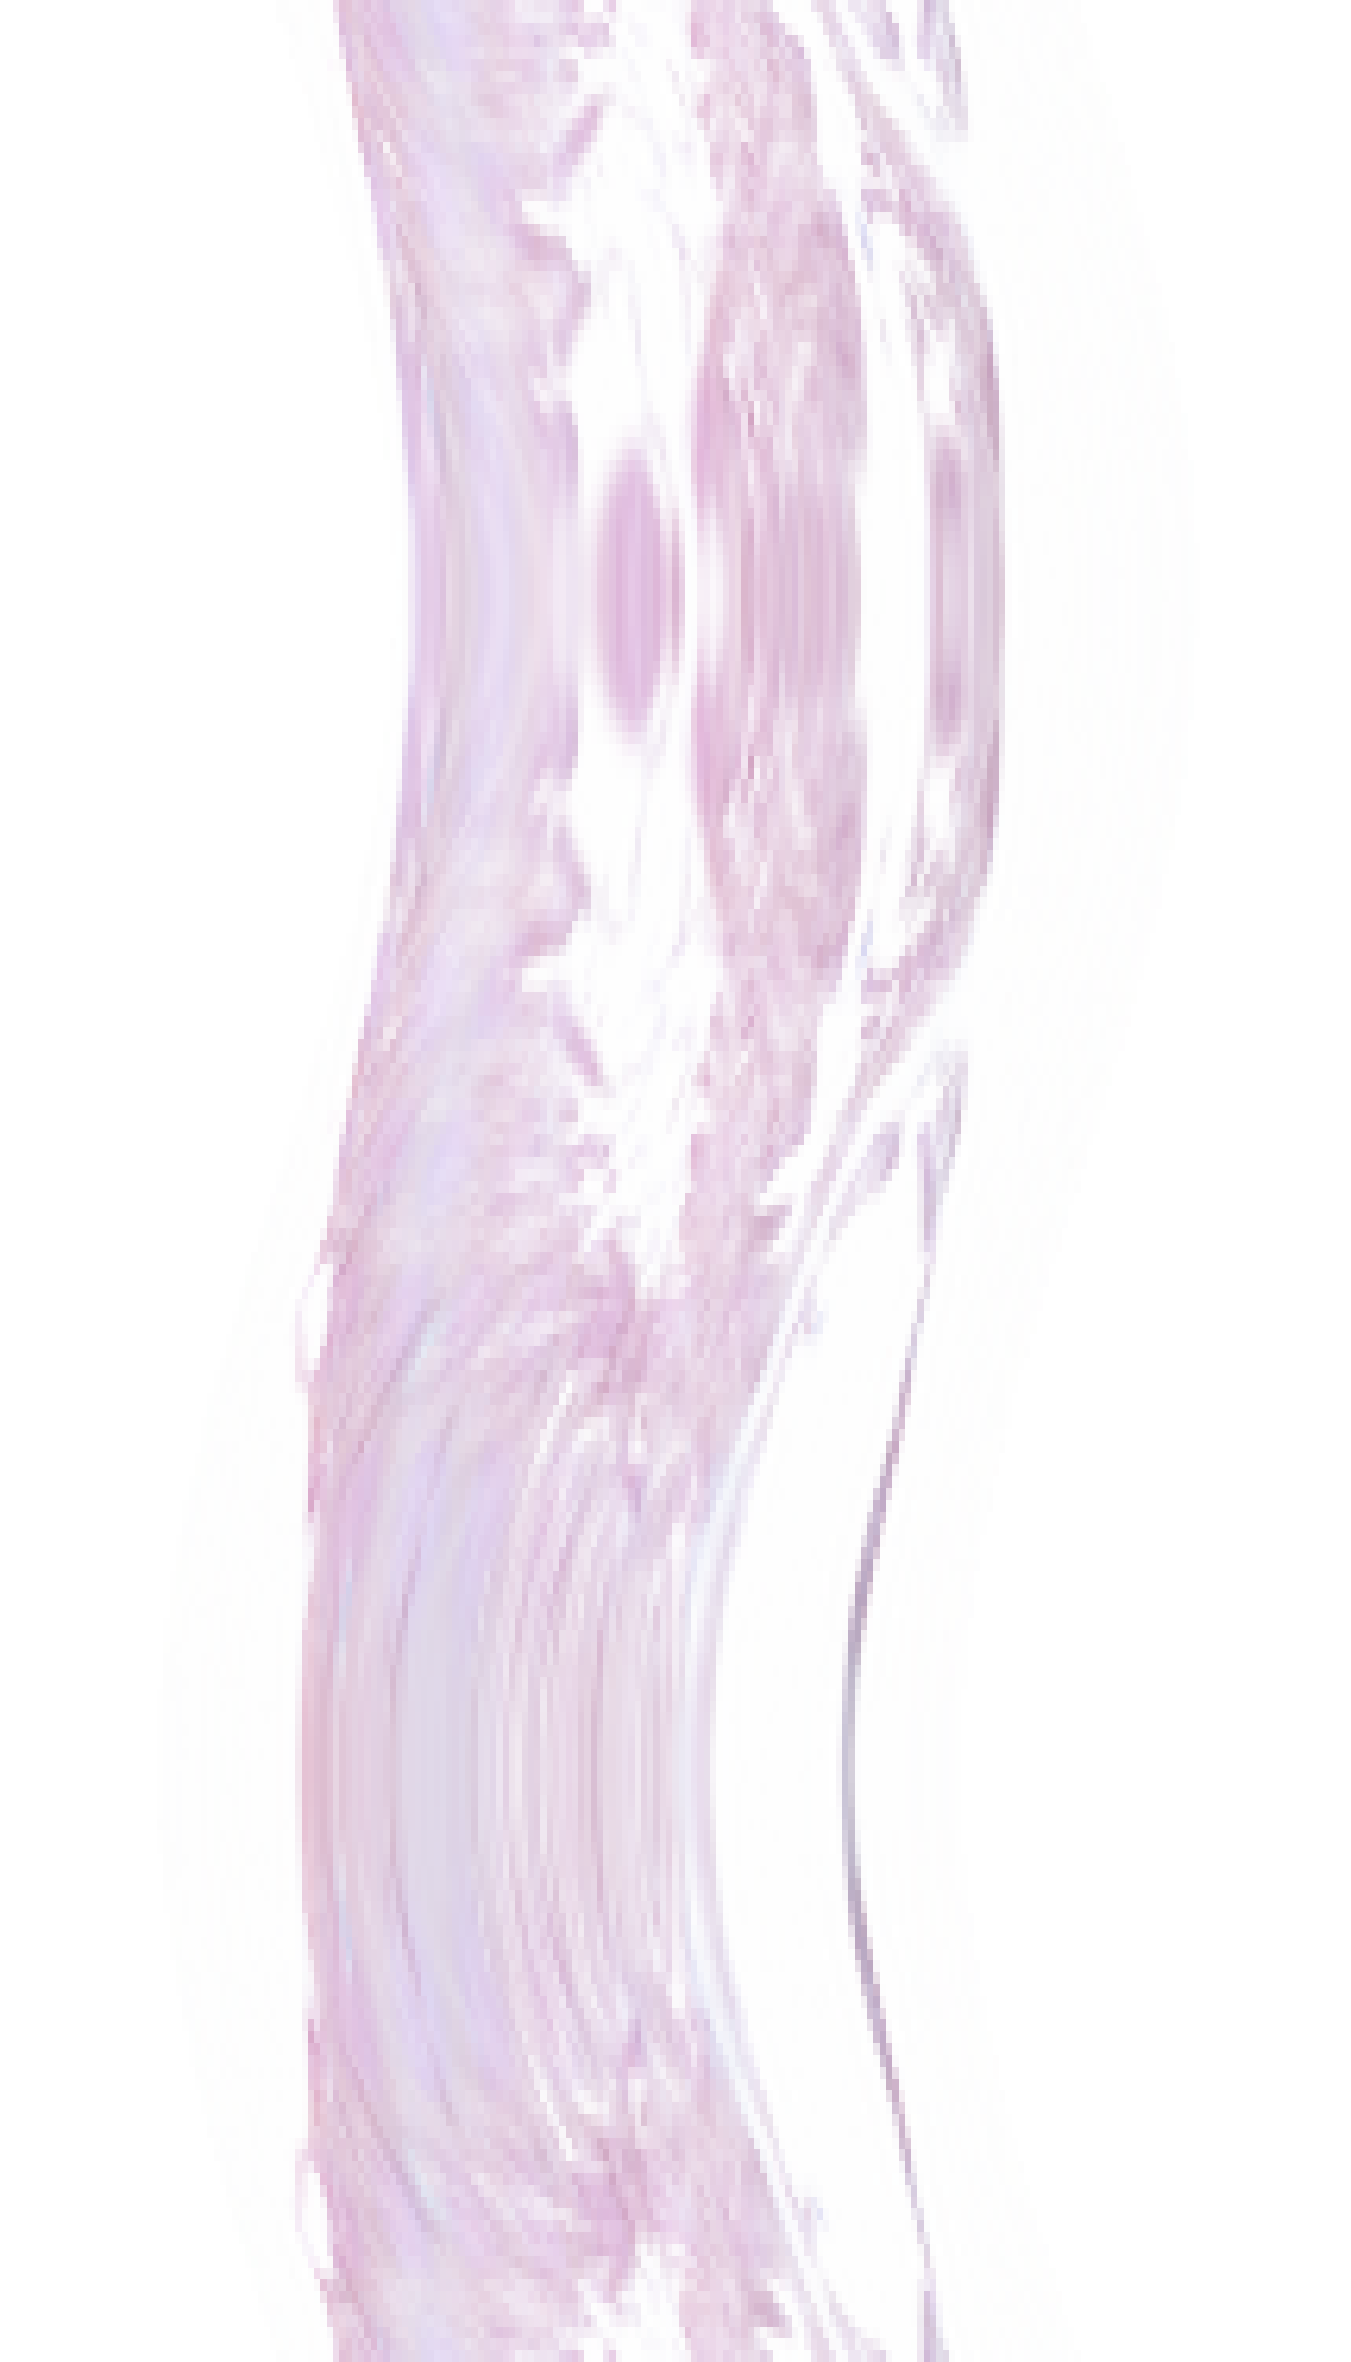
\includegraphics[height=0.33\textheight,type=pdf,ext=.pdf,read=.pdf]{Ch7/Figs/dummies/cross_section_perfect_200_alpha0.4t_0_088}}
    \caption{What a nice figure!}
    \label{fig:dummy_cross_sections}
  \end{sidewaysfigure}
  
  \begin{sidewaysfigure}[htbp]
    \centering
    \subfigure[][0 iterations]{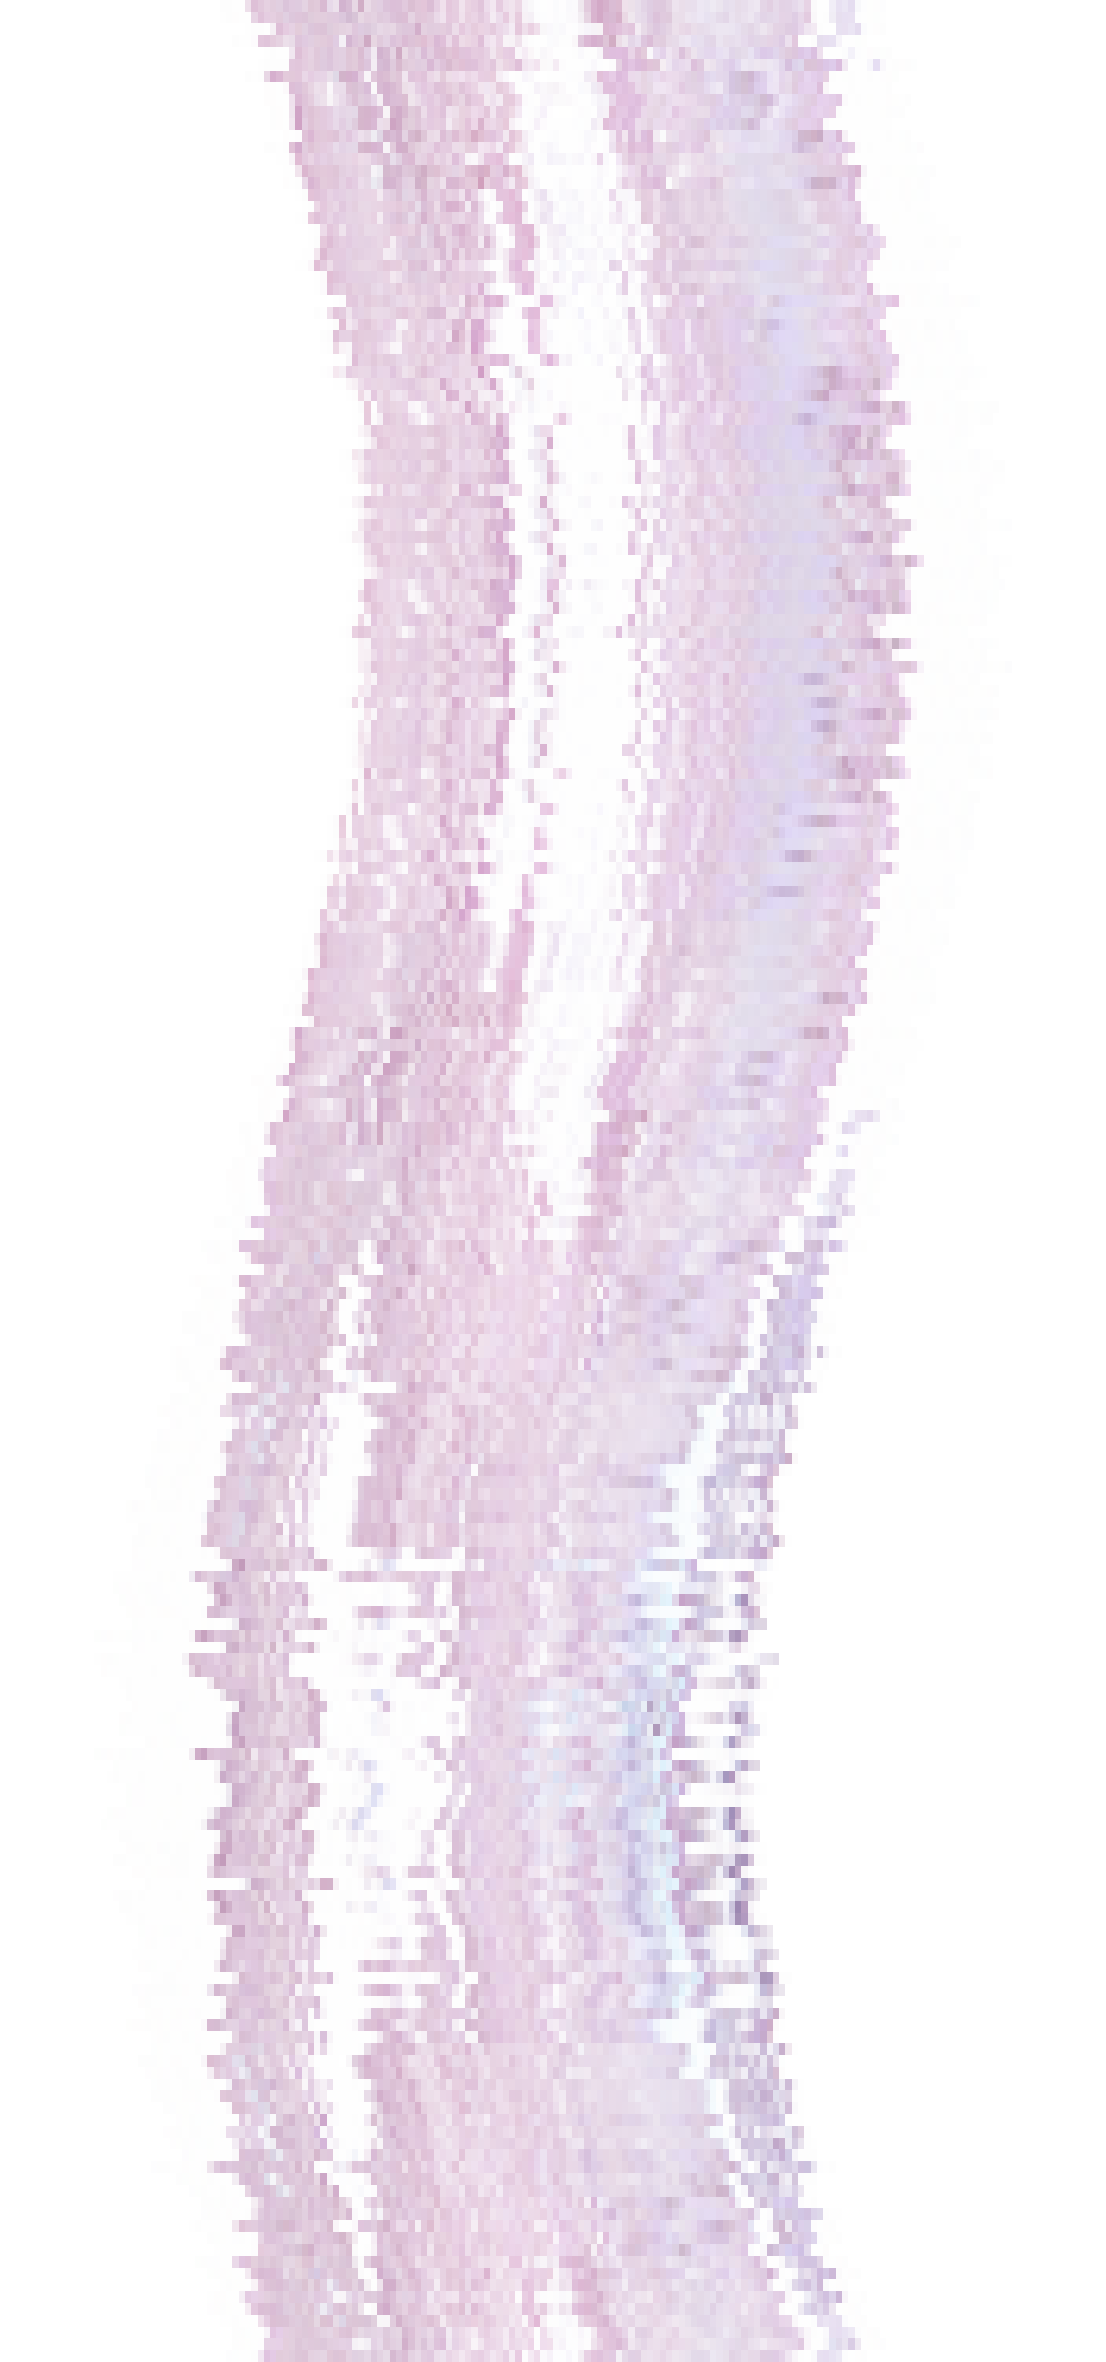
\includegraphics[height=0.33\textheight,type=pdf,ext=.pdf,read=.pdf]{Ch7/Figs/dummies/cross_section_200_alpha0.4t_0_1_107}}
    \subfigure[][1 iteration]{\includegraphics[height=0.33\textheight,type=pdf,ext=.pdf,read=.pdf]{Ch7/Figs/dummies/cross_section_200_alpha0.4t_1_1_107}}
    \subfigure[][3 iterations]{\includegraphics[height=0.33\textheight,type=pdf,ext=.pdf,read=.pdf]{Ch7/Figs/dummies/cross_section_200_alpha0.4t_3_1_107}}
    \subfigure[][10 iterations]{\includegraphics[height=0.33\textheight,type=pdf,ext=.pdf,read=.pdf]{Ch7/Figs/dummies/cross_section_200_alpha0.4t_10_1_107}}
    \subfigure[][without noise]{\includegraphics[height=0.33\textheight,type=pdf,ext=.pdf,read=.pdf]{Ch7/Figs/dummies/cross_section_perfect_200_alpha0.4t_1_107}}
    \caption{What a nice figure!}
    \label{fig:dummy_cross_sections}
  \end{sidewaysfigure}
    
  % rotated and translated
  \begin{sidewaysfigure}[htbp]
    \centering
    \subfigure[][0 iterations]{\includegraphics[height=0.33\textheight,type=pdf,ext=.pdf,read=.pdf]{Ch7/Figs/dummies/cross_section_200_alpha0.4rt_0_0_088}}
    \subfigure[][1 iteration]{\includegraphics[height=0.33\textheight,type=pdf,ext=.pdf,read=.pdf]{Ch7/Figs/dummies/cross_section_200_alpha0.4rt_1_0_088}}
    \subfigure[][3 iterations]{\includegraphics[height=0.33\textheight,type=pdf,ext=.pdf,read=.pdf]{Ch7/Figs/dummies/cross_section_200_alpha0.4rt_3_0_088}}
    \subfigure[][10 iterations]{\includegraphics[height=0.33\textheight,type=pdf,ext=.pdf,read=.pdf]{Ch7/Figs/dummies/cross_section_200_alpha0.4rt_10_0_088}}
    \subfigure[][without noise]{\includegraphics[height=0.33\textheight,type=pdf,ext=.pdf,read=.pdf]{Ch7/Figs/dummies/cross_section_perfect_200_alpha0.4rt_0_088}}
    \caption{What a nice figure! Notice a quarter of the way up from the base, a bad registration between 1 and 3 has been corrected in 10.}
    \label{fig:dummy_cross_sections}
  \end{sidewaysfigure}
  
  \begin{sidewaysfigure}[htbp]
    \centering
    \subfigure[][0 iterations]{\includegraphics[height=0.33\textheight,type=pdf,ext=.pdf,read=.pdf]{Ch7/Figs/dummies/cross_section_200_alpha0.4rt_0_1_107}}
    \subfigure[][1 iteration]{\includegraphics[height=0.33\textheight,type=pdf,ext=.pdf,read=.pdf]{Ch7/Figs/dummies/cross_section_200_alpha0.4rt_1_1_107}}
    \subfigure[][3 iterations]{\includegraphics[height=0.33\textheight,type=pdf,ext=.pdf,read=.pdf]{Ch7/Figs/dummies/cross_section_200_alpha0.4rt_3_1_107}}
    \subfigure[][10 iterations]{\includegraphics[height=0.33\textheight,type=pdf,ext=.pdf,read=.pdf]{Ch7/Figs/dummies/cross_section_200_alpha0.4rt_10_1_107}}
    \subfigure[][without noise]{\includegraphics[height=0.33\textheight,type=pdf,ext=.pdf,read=.pdf]{Ch7/Figs/dummies/cross_section_perfect_200_alpha0.4rt_1_107}}
    \caption{What a nice figure! Notice a quarter of the way up from the base, a bad registration between 1 and 3 has been corrected in 10}
    \label{fig:dummy_cross_sections}
  \end{sidewaysfigure}
  
  % colour slice differences
  \begin{sidewaysfigure}[htbp]
    \centering
    \subfigure[][unperturbed image]{\includegraphics[height=0.3\textheight,type=pdf,ext=.pdf,read=.pdf]{Ch7/Figs/dummies/colour_perfect_slice}} \quad
    \subfigure[][image with transformational noise]{\includegraphics[height=0.3\textheight,type=pdf,ext=.pdf,read=.pdf]{Ch7/Figs/dummies/colour_noisy_slice}} \\
    \subfigure[][squared differences in intensities]{\includegraphics[height=0.3\textheight,type=pdf,ext=.pdf,read=.pdf]{Ch7/Figs/dummies/colour_red_blue_diff}} \quad
    \subfigure[][squared differences in intensities]{\includegraphics[height=0.3\textheight,type=pdf,ext=.pdf,read=.pdf]{Ch7/Figs/dummies/colour_squared_diff}}
    \caption{slice 99 of straight volume. mean squared difference in bw image: 61.5265135808}
    \label{fig:dummy_cross_sections}
  \end{sidewaysfigure}
  
  % segmentation slice differences
  \begin{sidewaysfigure}[htbp]
    \centering
    \subfigure[][unperturbed image]{\includegraphics[height=0.3\textheight,type=pdf,ext=.pdf,read=.pdf]{Ch7/Figs/dummies/segmentation_perfect_slice}} \quad
    \subfigure[][image with transformational noise]{\includegraphics[height=0.3\textheight,type=pdf,ext=.pdf,read=.pdf]{Ch7/Figs/dummies/segmentation_noisy_slice}} \\
    \subfigure[][squared differences in intensities]{\includegraphics[height=0.3\textheight,type=pdf,ext=.pdf,read=.pdf]{Ch7/Figs/dummies/segmentation_red_blue_diff}} \quad
    \subfigure[][squared differences in intensities]{\includegraphics[height=0.3\textheight,type=pdf,ext=.pdf,read=.pdf]{Ch7/Figs/dummies/segmentation_squared_diff}}
    \caption{slice 99 of straight volume, reconstructed using manual segmentation. mean squared difference in bw image: 12.9321}
    \label{fig:dummy_cross_sections}
  \end{sidewaysfigure}
  
  % segmentation mean squared differences 3D
  \begin{sidewaysfigure}[htbp]
    \centering
    \subfigure[][straight column]{\includegraphics[height=0.33\textheight,type=pdf,ext=.pdf,read=.pdf]{Ch7/Figs/dummies/segmentation_mean_square_differences_3D}}
    \subfigure[][rotation]{\includegraphics[height=0.33\textheight,type=pdf,ext=.pdf,read=.pdf]{Ch7/Figs/dummies/segmentation_mean_square_differences_3Dr}}
    \subfigure[][translation]{\includegraphics[height=0.33\textheight,type=pdf,ext=.pdf,read=.pdf]{Ch7/Figs/dummies/segmentation_mean_square_differences_3Dt}}
    \subfigure[][rotation and translation]{\includegraphics[height=0.33\textheight,type=pdf,ext=.pdf,read=.pdf]{Ch7/Figs/dummies/segmentation_mean_square_differences_3Drt}}
    \caption{3D evolution of mean squared difference. Discuss how, as is visible in the colour and segmentation mean squared difference slices, even though registration was performed with the colour image, mean squared differences were calculated with the segmentation, and the results are much less noisy and clearer.}
    \label{fig:dummy_cross_sections}
  \end{sidewaysfigure}
  
  % segmentation mean squared differences 2D
  \begin{sidewaysfigure}[htbp]
    \centering
    \subfigure[][straight column]{\includegraphics[height=0.33\textheight,type=pdf,ext=.pdf,read=.pdf]{Ch7/Figs/dummies/segmentation_mean_square_differences_2D}}
    \subfigure[][rotation]{\includegraphics[height=0.33\textheight,type=pdf,ext=.pdf,read=.pdf]{Ch7/Figs/dummies/segmentation_mean_square_differences_2Dr}}
    \subfigure[][translation]{\includegraphics[height=0.33\textheight,type=pdf,ext=.pdf,read=.pdf]{Ch7/Figs/dummies/segmentation_mean_square_differences_2Dt}}
    \subfigure[][rotation and translation]{\includegraphics[height=0.33\textheight,type=pdf,ext=.pdf,read=.pdf]{Ch7/Figs/dummies/segmentation_mean_square_differences_2Drt}}
    \caption{Comment on magnitude and spectrum of error (higher frequencies filtered out)}
    \label{fig:dummy_cross_sections}
  \end{sidewaysfigure}
  
  % colour mean squared differences 3D
  \begin{sidewaysfigure}[htbp]
    \centering
    \subfigure[][straight column]{\includegraphics[height=0.33\textheight,type=pdf,ext=.pdf,read=.pdf]{Ch7/Figs/dummies/colour_mean_square_differences_3D}}
    \subfigure[][rotation]{\includegraphics[height=0.33\textheight,type=pdf,ext=.pdf,read=.pdf]{Ch7/Figs/dummies/colour_mean_square_differences_3Dr}}
    \subfigure[][translation]{\includegraphics[height=0.33\textheight,type=pdf,ext=.pdf,read=.pdf]{Ch7/Figs/dummies/colour_mean_square_differences_3Dt}}
    \subfigure[][rotation and translation]{\includegraphics[height=0.33\textheight,type=pdf,ext=.pdf,read=.pdf]{Ch7/Figs/dummies/colour_mean_square_differences_3Drt}}
    \caption{}
    \label{fig:dummy_cross_sections}
  \end{sidewaysfigure}
  
  % colour mean squared differences 2D
  \begin{sidewaysfigure}[htbp]
    \centering
    \subfigure[][straight column]{\includegraphics[height=0.33\textheight,type=pdf,ext=.pdf,read=.pdf]{Ch7/Figs/dummies/colour_mean_square_differences_2D}}
    \subfigure[][rotation]{\includegraphics[height=0.33\textheight,type=pdf,ext=.pdf,read=.pdf]{Ch7/Figs/dummies/colour_mean_square_differences_2Dr}}
    \subfigure[][translation]{\includegraphics[height=0.33\textheight,type=pdf,ext=.pdf,read=.pdf]{Ch7/Figs/dummies/colour_mean_square_differences_2Dt}}
    \subfigure[][rotation and translation]{\includegraphics[height=0.33\textheight,type=pdf,ext=.pdf,read=.pdf]{Ch7/Figs/dummies/colour_mean_square_differences_2Drt}}
    \caption{}
    \label{fig:dummy_cross_sections}
  \end{sidewaysfigure}
  
  
  this is a load of content
  
  this is a load of content
  
  this is a load of content
  
  this is a load of content
  
  this is a load of content
  
  this is a load of content
  
  this is a load of content
  
  this is a load of content
  
  this is a load of content
  
  this is a load of content
  
  this is a load of content
  
  this is a load of content
  
  % old result
  \begin{sidewaysfigure}[htbp]
    \centering
    \subfigure[][0 iterations]{\includegraphics[height=0.33\textheight,type=pdf,ext=.pdf,read=.pdf]{Ch7/Figs/dummies/low_noise_with_original_images_cross_section_200_alpha0.4rt_0_0_088}}
    \subfigure[][1 iteration]{\includegraphics[height=0.33\textheight,type=pdf,ext=.pdf,read=.pdf]{Ch7/Figs/dummies/low_noise_with_original_images_cross_section_200_alpha0.4rt_1_0_088}}
    \subfigure[][3 iterations]{\includegraphics[height=0.33\textheight,type=pdf,ext=.pdf,read=.pdf]{Ch7/Figs/dummies/low_noise_with_original_images_cross_section_200_alpha0.4rt_3_0_088}}
    \subfigure[][10 iterations]{\includegraphics[height=0.33\textheight,type=pdf,ext=.pdf,read=.pdf]{Ch7/Figs/dummies/low_noise_with_original_images_cross_section_200_alpha0.4rt_10_0_088}}
    \subfigure[][without noise]{\includegraphics[height=0.33\textheight,type=pdf,ext=.pdf,read=.pdf]{Ch7/Figs/dummies/low_noise_with_original_images_cross_section_perfect_200_alpha0.4rt_0_088}}
    \caption{What a nice figure! Notice a quarter of the way up from the base, a bad registration between 1 and 3 has been corrected in 10. This demonstrates that even when the cost function of the registration is spiky, and results of a single run are sensitive to initialisation, the iterative nature of the diffusion algorithm greatly improves robustness by providing multiple opportunities to escape local minima.}
    \label{fig:dummy_cross_sections}
  \end{sidewaysfigure}
  
  

  this is a load of content
  
  this is a load of content
  
  this is a load of content
  
  this is a load of content
  
  this is a load of content
  
  this is a load of content
  
  
  this is a load of content
  
  this is a load of content
  
  this is a load of content
  
  this is a load of content
  
  this is a load of content
  
  this is a load of content
  
  
  this is a load of content
  
  this is a load of content
  
  this is a load of content
  
  this is a load of content
  
  this is a load of content
  
  this is a load of content
  
  
  this is a load of content
  
  this is a load of content
  
  this is a load of content
  
  this is a load of content
  
  this is a load of content
  
  this is a load of content
  
  
  this is a load of content
  
  this is a load of content
  
  this is a load of content
  
  this is a load of content
  
  this is a load of content
  
  this is a load of content
  
  
  this is a load of content
  
  this is a load of content
  
  this is a load of content
  
  this is a load of content
  
  this is a load of content
  
  this is a load of content
  

  % full contours
  % \begin{figure}[htbp]\texttt{}
  %   \centering
  %   \subfigure[][]{\includegraphics[width=0.4\pagewidth]{Ch7/Figs/dummies/contours/whole_surface_0}}
  %   \subfigure[][]{\includegraphics[width=0.4\pagewidth]{Ch7/Figs/dummies/contours/whole_surface_10}}
  %   \caption{What a nice figure!}
  %   \label{fig:test.png}
  % \end{figure}
  % 
  % \begin{figure}[htbp]
  %   \centering
  %   \subfigure[][]{\includegraphics[width=0.4\pagewidth]{Ch7/Figs/dummies/contours/whole_surfacer_0}}
  %   \subfigure[][]{\includegraphics[width=0.4\pagewidth]{Ch7/Figs/dummies/contours/whole_surfacer_10}}
  %   \caption{What a nice figure!}
  %   \label{fig:test.png}
  % \end{figure}
  % 
  % \begin{figure}[htbp]
  %   \centering
  %   \subfigure[][]{\includegraphics[width=0.4\pagewidth]{Ch7/Figs/dummies/contours/whole_surfacet_0}}
  %   \subfigure[][]{\includegraphics[width=0.4\pagewidth]{Ch7/Figs/dummies/contours/whole_surfacet_10}}
  %   \caption{What a nice figure!}
  %   \label{fig:test.png}
  % \end{figure}
  % 
  \begin{figure}[htbp]
    \centering
    \subfigure[][]{\includegraphics[width=0.4\pagewidth]{Ch7/Figs/dummies/contours/whole_surfacert_0}}
    \subfigure[][]{\includegraphics[width=0.4\pagewidth]{Ch7/Figs/dummies/contours/whole_surfacert_10}}
    \caption{This is a figure!}
    \label{fig:test.png}
  \end{figure}
  
  It is worth noting that the adjustment algorithm itself is stable with much larger levels of noise than shown here, comparable to those in Figures~\ref{fig:1d_diffusion_0_40}, \ref{fig:1d_diffusion_0_49}, \ref{fig:1d_diffusion_0_50} and \ref{fig:1d_diffusion_0_51}. It is simply that the registration is sensitive, wouldn't work blah blah.
  
  Parameters used for noisy dummies were x, y, z. The important factor is whether the slice-to-slice registrations are quickly and robustly successful, and so much greater noise could be filtered by the algorithm, as long as the parameters were tuned for large displacements for the first few iterations, and then smaller displacements for the finer smoothing in the later iterations.
  
  Prove that random walk is binomial distribution, which tends to Gaussian distribution, therefore with enough iterations we are applying gaussian transformational smoothing to the volume.
  
  Particles undergoing brownian motion diffuse, hence the name.
  
  % `http://en.wikipedia.org/wiki/Random_walk#One-dimensional_random_walk'
  1D analogy of diffusion and noise filtering, with sine wave and overlayed noise, and diagram
  
  Figure of banana-effect registration
  
  Anisotropic diffusion: 
  
  Divide MRI into slices, then apply artificial noise, then compare banana registration to diffusion registration.
  
  Pull image from Evernote
  
      Figure~\ref{fig:noisy-sine-wave}
      \begin{figure}[htbp]
        \centering
        \includegraphics[height=0.7\textwidth]{Ch6/Figs/process_diagram}
        \caption{A numerical approximation of a sine wave, on 1000 equispaced points from $0$ to $2\pi$. Random noise from a Gaussian distribution is added, with variance equal to the amplitude of the sine wave.}
      \end{figure}
    
  \subsection{2D Transforms Diffusion} % (fold)
  \label{sub:2d_transforms_diffusion}
    This 1-dimensional model is trivially extended to a 2D translation of a slice image aligning with its neighbour, since both of the parameters are mutually orthogonal. But what about the more complex harder with say affine transform. Square root of transform blah blah.
  
  % subsection 2d_transforms_diffusion (end)
  
% section methods (end)

\section{Results} % (fold)
\label{sec:results}
  
  Figures:
  
  % x slices
  \begin{figure}[htbp]
    \centering
    \subfigure[][]{\includegraphics[height=0.31\textheight]{Ch7/Figs/adjusted_0_0_235}}
    \subfigure[][]{\includegraphics[height=0.31\textheight]{Ch7/Figs/adjusted_1_0_235}}
    \subfigure[][]{\includegraphics[height=0.31\textheight]{Ch7/Figs/adjusted_20_0_235}}
    \caption{Cross-section after 0, 1 and 20 iterations of diffusion}
    \label{fig:adjusted_0_235}
  \end{figure}

  % y slices
  \begin{figure}[htbp]
    \centering
    \subfigure[][]{\includegraphics[height=0.31\textheight]{Ch7/Figs/adjusted_0_1_287}}
    \subfigure[][]{\includegraphics[height=0.31\textheight]{Ch7/Figs/adjusted_1_1_287}}
    \subfigure[][]{\includegraphics[height=0.31\textheight]{Ch7/Figs/adjusted_20_1_287}}
    \caption{Cross-section after 0, 1 and 20 iterations of diffusion}
    \label{fig:adjusted_1_287}
  \end{figure}
  
  % lower 100 slices zoom
  % x slices
  \begin{sidewaysfigure}[htbp]
    \centering
    \subfigure[][]{\includegraphics[height=0.15\textheight]{Ch7/Figs/adjusted_0_0_235_zoomed}}
    \subfigure[][]{\includegraphics[height=0.15\textheight]{Ch7/Figs/adjusted_1_0_235_zoomed}}
    \subfigure[][]{\includegraphics[height=0.15\textheight]{Ch7/Figs/adjusted_20_0_235_zoomed}}
    \caption{Lower 100 slices of cross-section after 0, 1 and 20 iterations of diffusion}
    \label{fig:adjusted_0_235}
  \end{sidewaysfigure}

  % y slices
  \begin{sidewaysfigure}[htbp]
    \centering
    \subfigure[][]{\includegraphics[height=0.15\textheight]{Ch7/Figs/adjusted_0_1_287_zoomed}}
    \subfigure[][]{\includegraphics[height=0.15\textheight]{Ch7/Figs/adjusted_1_1_287_zoomed}}
    \subfigure[][]{\includegraphics[height=0.15\textheight]{Ch7/Figs/adjusted_20_1_287_zoomed}}
    \caption{Lower 100 slices of cross-section after 0, 1 and 20 iterations of diffusion}
    \label{fig:adjusted_1_287}
  \end{sidewaysfigure}
  
  % diffused contours
  \begin{sidewaysfigure}[p]
    \centering
    \subfigure[][]{\includegraphics[width=0.9\textheight]{Ch7/Figs/Rat28/contours/whole_positive_x_diffused}}
    \caption{}
    \label{fig:image1.png}
  \end{sidewaysfigure}

  \begin{sidewaysfigure}[p]
    \centering
    \subfigure[][]{\includegraphics[width=0.9\textheight]{Ch7/Figs/Rat28/contours/whole_negative_x_diffused}}
    \caption{}
    \label{fig:image1.png}
  \end{sidewaysfigure}

  \begin{sidewaysfigure}[p]
    \centering
    \subfigure[][]{\includegraphics[width=0.9\textheight]{Ch7/Figs/Rat28/contours/whole_positive_y_diffused}}
    \caption{}
    \label{fig:image1.png}
  \end{sidewaysfigure}

  \begin{sidewaysfigure}[p]
    \centering
    \subfigure[][]{\includegraphics[width=0.9\textheight]{Ch7/Figs/Rat28/contours/whole_positive_z_diffused}}
    \caption{}
    \label{fig:image1.png}
  \end{sidewaysfigure}

  
  
  2 cross-sections and a contour surface of:
    the straight column, rotation, translation, rotation + translation volumes
      with perfect, noisy, smoothed 0.4, smoothed 0.3
        
  Figure of 0.4 200rt plot\_metric\_values\_and\_differences from the first step, showing that all the registrations are reaching their minimum of around the same low metric value, it's just that the computation of the Adjusted Transforms is unstable.
  
  
  
  
  \subsection{Regional Registration} % (fold)
  \label{sub:regional_registration}
    Segment a largish blood vessel or vessel branch in the histology and show that it looks like a smooth surface and is aligned. 
  % subsection regional_registration (end)

% section results (end)

\section{Discussion} % (fold)
\label{sec:discussion}
  GENERAL POINT, `it will be shown later' in introductory paragraphs, to tittilate the reader.

  With a better interpolation scheme, it might be possible to crank alpha up further.
  
  Inherently introduces the banana problem across the curvature of the heart (~30 slices - give justification with numbers)
  Can only be used for small adjustments, given non-commutativity of operators etc.
  Figures and evaluation of results e.g. examples of great and bad slice-pair registrations, maybe one slice has a large abberation. Works better for different regions? e.g. round blob versus cavity?
  Alternative Implementations:
  Could register to more than just nearest neighbours at each iteration, although multiple iterations of nearest neighbour is equivalent to this, requires the same total number of slice-to-slice iterations, and is more stable and accurate, as errors from the first nearest neighbour iteration due to e.g. interpolation error, random noise etc. are mitigated by subsequent iterations.
  Expensive to rerun slice-pair registrations every iteration, could infer from previous registration. Inaccuracy and instability?
  
  Could be extended easily to more complex transforms such as b-spline, although perhaps a little trickier to think about interpolating transforms other than linearly interpolating their parameters.

% section discussion (end)


  
% subsection slice_to_slice_diffusion_smoothing_algorithm (end)

